
%% This is file `elsarticle-template-2-harv.tex',
%%
%% Copyright 2009 Elsevier Ltd
%%
%% This file is part of the 'Elsarticle Bundle'.
%% ---------------------------------------------
%%
%% It may be distributed under the conditions of the LaTeX Project Public
%% License, either version 1.2 of this license or (at your option) any
%% later version.  The latest version of this license is in
%%    http://www.latex-project.org/lppl.txt
%% and version 1.2 or later is part of all distributions of LaTeX
%% version 1999/12/01 or later.
%%
%% The list of all files belonging to the 'Elsarticle Bundle' is
%% given in the file `manifest.txt'.
%%
%% Template article for Elsevier's document class `elsarticle'
%% with harvard style bibliographic references
%%
%% $Id: elsarticle-template-2-harv.tex 155 2009-10-08 05:35:05Z rishi $
%% $URL: http://lenova.river-valley.com/svn/elsbst/trunk/elsarticle-template-2-harv.tex $
%%
%%\documentclass[preprint,authoryear,12pt]{elsarticle}

%% Use the option review to obtain double line spacing
\documentclass[authoryear,preprint,review,12pt]{elsarticle}

%% Use the options 1p,twocolumn; 3p; 3p,twocolumn; 5p; or 5p,twocolumn
%% for a journal layout:
%% \documentclass[final,authoryear,1p,times]{elsarticle}
%% \documentclass[final,authoryear,1p,times,twocolumn]{elsarticle}
%% \documentclass[final,authoryear,3p,times]{elsarticle}
%% \documentclass[final,authoryear,3p,times,twocolumn]{elsarticle}
%%\documentclass[final,authoryear,5p,times]{elsarticle}
%\documentclass[final,authoryear,5p,times,twocolumn]{elsarticle}
\usepackage{textcomp, fixltx2e}

%% if you use PostScript figures in your article
%% use the graphics package for simple commands
%% \usepackage{graphics}
%% or use the graphicx package for more complicated commands
%% \usepackage{graphicx}
%% or use the epsfig package if you prefer to use the old commands
%% \usepackage{epsfig}

\usepackage{fullpage}

%% The amssymb package provides various useful mathematical symbols
\usepackage{amssymb}


%% The amsthm package provides extended theorem environments
%% \usepackage{amsthm}

%% The lineno packages adds line numbers. Start line numbering with
%% \begin{linenumbers}, end it with \end{linenumbers}. Or switch it on
%% for the whole article with \linenumbers after \end{frontmatter}.
%% \usepackage{lineno}

%% natbib.sty is loaded by default. However, natbib options can be
%% provided with \biboptions{...} comman. Following options are
%% valid:

%%   round  -  round parentheses are used (default)
%%   square -  square brackets are used   [option]
%%   curly  -  curly braces are used      {option}
%%   angle  -  angle brackets are used    <option>
%%   semicolon  -  multiple citations separated by semi-colon (default)
%%   colon  - same as semicolon, an earlier confusion
%%   comma  -  separated by comma
%%   authoryear - selects author-year citations (default)
%%   numbers-  selects numerical citations
%%   super  -  numerical citations as superscripts
%%   sort   -  sorts multiple citations according to order in ref. list
%%   sort&compress   -  like sort, but also compresses numerical citations
%%   compress - compresses without sorting
%%   longnamesfirst  -  makes first citation full author list
%%
%% \biboptions{longnamesfirst,comma}

 \biboptions{round}

 \journal{Soil Biology and Biochemistry}

\begin{document}

\begin{frontmatter}

%% Title, authors and addresses

%% use the tnoteref command within \title for footnotes;
%% use the tnotetext command for the associated footnote;
%% use the fnref command within \author or \address for footnotes;
%% use the fntext command for the associated footnote;
%% use the corref command within \author for corresponding author footnotes;
%% use the cortext command for the associated footnote;
%% use the ead command for the email address,
%% and the form \ead[url] for the home page:
%%
%% \title{Title\tnoteref{label1}}
%% \tnotetext[label1]{}
%% \author{Name\corref{cor1}\fnref{label2}}
%% \ead{email address}
%% \ead[url]{home page}
%% \fntext[label2]{}
%% \cortext[cor1]{}
%% \address{Address\fnref{label3}}
%% \fntext[label3]{}

\title{Resource control over early lignin decomposition in beech litter}

%% use optional labels to link authors explicitly to addresses:
%% \author[label1,label2]{<author name>}
%% \address[label1]{<address>}
%% \address[label2]{<address>}

%\author{}

% \author[1]{Lukas Kohl}
% \author[1]{Maria Mooshammer}
% \author[1]{Sonja Leitner}
% \author[1]{Ieda H\"ammerle-N.}
% \author[1]{Alexander Frank}
% \author[1]{Lucia Fuchslueger}
% \author[1]{J\"org Schnecker}
% \author[2]{Katharina Keiblinger}
% \author[2]{Sophie Zechmeister-Boltenstern}
% \author[1]{Wolfgang Wanek}
% \author[1]{Andreas Richter}
%%%>>>>corresponding author?!
\author[1]{me}
\author[2]{and my friends}

\address[1]{Checo}
% \address[2]{BFW}
\address[2]{not Checo}


\address{}


\begin{abstract}
The degradation of plant polymers in litter decay determines quality and quantity of recalcitrant carbon input to soils. Nevertheless, the involved transformations remain unclear. Beech litter from four different sites, varying in N, P and inital soluble C content was incubated over 15 month. We follow the accumulation or depletion of lignin, carbohydrates and other lipophilic compounds by pyrolysis-GC/MS. 
In three of the four sites, we found a clear preference of carbohydrates over lignin decomposition during the first 6 month. The fourth site, characterized by low N and high soluble C content, shows no such preference, degrading lignin at the same rate as bulk litter biomass.


\end{abstract}

\begin{keyword}
%% keywords here, in the form: 
litter decomposition \sep lignin \sep analytical pyrolysis \sep Py-GC/MS

%% MSC codes here, in the form: \MSC code \sep code
%% or \MSC[2008] code \sep code (2000 is the default)

\end{keyword}

\end{frontmatter}

%\linenumbers

%% main text
\section{Introduction}

Plant litter biomass is dominated by macromolecular compounds. Together, lignin, carbohydrate and protein polymers make up xx\% of litter dry mass, while leach-able substances (``DOM'') in litter account for only xx \%. The conversion of insoluble compounds in particular organic matter (``POM'') into soluble substances is key process in litter decomposition: Microorganisms can only metabolize DOM directly, but rely on the excretion of extracellular enzymes to convert POM in DOM \citep{Klotzbucher2011,Bengtson2007,Marschner2003}.

Carbohydrates and protein polymerization is exactly controlled by catalytic enzymes. Lignin is result of a radical polymerization reaction of enzyme-activated hydroypropylphenol monomers. During lignin condensation other compounds - most prominently carbohydrates and protein - are incorporated into lignin structures \citep{Achyuthan2010}. Extracted (ADF) lignin fractions from fresh beech litter were found to have nitrogen contents twice as high as in bulk litter \citep{Dyckmans2002}. 

Conventional litter decomposition models [lit] follow the idea that macromolecules in litter form three independent carbon pools of increasing recalcitrance. These pools are attributed to (1) soluble compounds (most prominently starch), (2) cellulose and hemi-celluloses and (3) lignin. During decomposition, soluble compounds are easiest accessible for microbes and consumed first, followed by carbohydrates (i.e. cellulose). Lignin can be decomposed only by specialists and is not degraded until accumulated to a certain, critical level when it inhibits the degradation of other compounds \citep{Berg1980, Couteaux1995, Moorhead2006}.[more lit.] 

%[This concept was first described by , and stills forms the base of recent models and textbooks [lit!!hh]. 

One reason for the popularity of this model is that sizes of the three carbon pools can easily determined by proximate analysis. In these methods, litter cellulose, hemi-celluloses and lignin content are determined by sequential extractions with selective solvents. Especially for lignin determination, these methods (``Klason''- and ``ADF''-lignin) were repeatedly criticize as unspecific \citep{Hatfield2005}. When analyzed with alternative methods (NMR, CuO-oxidation, Pyrolysis-GC/MS), extracted lignin fractions contain many other than the proclaimed substances. (i.e. \cite{Preston1997}, [lit CuO], lit[Pyr]). However, while not helpful in tracking the fate of lignin in litter decomposition, these fractions - re-labeled ``acid un-hydrolyzable residues'' (AUR) - can be used as an indicator for the content of the most recalcitrant carbon compounds in litter \citep{Prescott2010}. For the lipids and plant waxes also found in AUR fraction, neither their accumulation/depletion during decomposition nor the effect of their concentration on decomposition processes is known [!check!,!lit!]

%[The question of reference material]

%While it is possible to determine carbohydrate and protein contents by enzymatic or chemical hydrolysis and quantification of monomers, due to the arbitrary structure of it's polymers, this approach can not be used for lignin determination.

%Especially lignin determination by this method has been citized extensively \citep{Hatfield2005}, as acid unsoluble residues (AUR, the fraction formally known as lignin) contain a number of hydrophobic compounds like cutin, surface waxes [fatty acids] and condesed tannins (lit). 

Recent studies using more specific methods to determine litter lignin content (CuO - oxidation, pyr-GC/MS, NMR) question the previously assumed intrinsic recalcitrance of lignin. Mean residence times for lignin in soils were calculated from both laboratory and outdoor incubation of litter/soil mixtures. Lignin residence times found were no longer than other carbon compounds or bulk SOM \citep{Thevenot2010a, Bol2009} [more lit?]. For litter, lignin decomposition rates were found not to increase from early to late decomposition stages \citep{Klotzbucher2011}. Based on these results, the authors propose a new model for lignin degradation: fastest lignin degradation in litter decay occurs during early litter decomposition; lignin decomposition during late decomposition is limited by (dissolved organic) carbon availability. 

Neither the traditional 3-pool models nor \cite{Klotzbucher2011} elaborate the effect of macro-nutrient (nitrogen and phosphorous) availability on lignin decomposition. Nitrogen fertilization experiments on litter and soils suggest that litter nitrogen content affects lignin degradation: N addition increases mass loss rates in low-lignin litter while slowing down decomposition in lignin-rich litter \citep{Knorr2005}. High nitrogen levels were reported to inhibit lignolytic enzyme in forest soils\citep{Sinsabaugh2010}. Cellulose addition lead to a higher mineralization of SOM in fertilized than in unfertilized soils \citep{Fontaine2011}. However, results of artificial fertilization can not be compared to different ``natural'' nutrient gradients. To our knowledge, no other experiment has yet compared effects of intra-specific variance in litter nutrient contents on decomposition processes. N-fertilization experiments can simulate increased N-deposition rates. To simulate variations litter C:N ratios, our approach is preferable, because potential changes in litter N content will most probably affect complex POM substrates. There, N location and accessibility is different of the low molecular weight N species available for fertilization experiments. 


% [Elevated N deposition and elevated soil N content increase litter N contents, while a recent meta-study hints that elevated atmospheric CO$_{2}$ concentrations cause wider litter C:N ratios \citep{Luo2006}. Therefore it is important to assess the impact of shifts in litter C:N ratio on decomposition processes and the chemical nature of the resulting organic matter to predict feedback mechanisms of anthropogenic alterations of global carbon and nitrogen cycles. While predictions of changes in mass loss rates under alternated litter C:N ratios are abound [lit.], no studies on changes in the quality of litter biomass during and after decomposition or of the dynamics of accumulation/depletion of fragments of the litter biomass during decomposition exist yet.]

%Also, interdependance of these pools seems much higher than expected. Lignified cellulose and protein is not accessable without degrading lignin... Ligin fractions extracted from (fresh) beech litter have beed demonstrated to have a very narrow C:N ratio if compared to bulk litter, nonligneous cell walls or soluble matter. It is assumed, that proteins are covalently bound to lignin polymers during polymerization. For litter decomposing microbia this implies that degrading lignin increases nitrogen availability, while degrading non-lignified carbohydrates yields more metabolic energy, but no additional nitrogen. In an incubation eperiment with a litter/soil mixture, N addition stimulated carbon mineralization during the first weeks of incubation but slowed it down duringThe after  with  ratios after climate chamber incubation for up to 15 month. late decomposition.

%In temperate forests, litter decomposition is generally considered nitrogen limited (lit).
%several experiments report retention times for lignin in soil [not much higher than other soil components].

Several recent studies apply analytical pyrolysis (Pyr-GC/MS) to characterize complex natural organic polymers like soil organic matter (SOM, \cite{Vancampenhout2010}[more lit here]). 
%Only a limited number of pyrolysis studies comparing different decomposition levels have been done. 
Pyrolysis-based decomposition studies usually focus on the woody material \citep{Vinciguerra2007} or  soil/litter mixtures [lit! - z.b. gleixner ca.1999]. Microbial decomposition of straw was followed by Pyr-GC/MS by [lit] We found only one study analyzing different stages of litter decomposition with analytical pyrolysis \citep{Franchini2002} and one recent study using a related technique (thermally assisted hydrolysis and methylation in \citep{Snajdr2011}. 

\cite{Kuder1998}

%European beech (\emph{Fagus silvaticus} L.) is the dominant forest building tree species in central europe. 
In this study we analyze samples of climate-chamber incubated beech litter varying in N and P content with Pyrolysis-GC/MS (pyr-GC/MS). The experiment was designed to study microbial decomposition, exclude decomposing fauna and keep climatic conditions constant. Extensive data on litter chemistry and and decomposition process rates are available for this samples from previously publications \citep{Mooshammer2011, Wanek2011, Leitner2011} as unpublished data [provided by the MicDiF national research network]. 

We focus on changes in lignin and carbohydrate content, assuming that

(1) Lignified biomass and non-lignified carbohydrates are alternatively degraded. Microorganisms have to allocate N in the production of different enzymes. When environmental conditions are constant, microbial substrate preference is determined by litter chemistry,

(2) While (non-lignified) carbohydrates are easier degraded than lignin and the resulting sugar monomers yield more energy, lignin degradation improves to accessibility of nitrogen (``lignin mining'', \cite{Craine2007}). 
 More lignin is decomposed when nitrogen availability is low, and high nitrogen availability inhibits lignin degradation.

(3) Lignin degradation is inhibited when little DOC is available and decomposition is energy limited (as proposed by \cite{Klotzbucher2011}). 

%Their accumulation and/or depletion during decomposition was extensively studied, nevertheless recent studies based on new methods to measure lignin content challange traditional models.

% Decomposition conditions control whether assimilated carbon is released immideately or sequestered to soil organic matter. Decomposition processes also control the quality of the resulting organic matter and therefore soil carbon recalcitrance. 

%\cite{Prescott2010} suggests the amount of remaining biomass more important than the decomposition speed. We suggest, the chemical nature of this remaining biomass might be a factor too. we should study the influences of environmental parametres on the chemical conposition of the remaining biomass. 

% but using methods based on detergent extraction no regarded unspecific. 

%Large scale experiments (lit!) conducted during the last years collected detailed data on chemical and ecological controls predict dry mass loss during litter decomposition. Nevertheless, understanding of chamical transformations in litter loss is still limited, as most studies limit their analysis of high molecular weight compounds to detergent extraction based methods (Klason Lignin, ... - lit). 


%\cite{Snajdr2011a} used THM (a pyrolysis-related method) in a litterbag expiriment, but limits analysis to determining lignin:carbohydrate ratios. 

%These studies often explain biomarkers found in SOM by their occurance in a plant polymers and propose a decendence from thos biomarkers \citep{Schellekens2009b}, some of them also analyze local vegetation for comparison.


% We follow three research questions:

%(1) To which does HMW carbon at different sites differ? 

%(2) Which substance classes are accumulaten/depleted during decomposition and is the rate of accumulation/depletion influences by nutrient compositoin? Nutrient addition studies show a decrease of phenole oxidizing enzymes (lit!), but those have not been shown in pyrolysis data yet.

%(3) Does HMW chemistry excercice control over decomposition processes? Do changes in HMW chemistry (i.e. accumulation of more recalcitrant substances) explain the decline of decomposition rates?




% Nitrogen availability has been shown to be rate limiting in beech litter (lit) ??\citep{Mooshammer2011}??.

%With increasing anthropogenic nitrogen deposition and contradicting studies on whether litter C:N ratio is change due to increasing anthmospheric CO$_2$ ratios, knowledge about effects of nutrient availability on the chemical properties of soil organic matter become increasingly relevant (lit.).

% Most experiments study nutrient control by fertilization. 
%Nutrient availability Litter stoichiometry...
%prescott -> metastudy zu litter CN aus den 90ern
%die aktuelle metastudy
%prescott N deposition 
%N-addition studys. few studies on stoichiometry in naturally variing systems.

% CN ratio changes >> 


\section{Material and methods}

\subsection{Litter decomposition experiment}
A detailed description of our litter decomposition experiment was published in \cite{Wanek2011}. Briefly, beech litter from four sites in Austria (Achenkirch (AK), Klausenleopoldsdorf(KL), Ossiach(OS), and Schottenwald(SW); refered to as litter types) was collected in October 2008. Litter was homogenized, sterilized and inoculated (1.5\% w/w) with a mixture of litter and soil to assure all litter types share the same initial microbial community. From each type, four samples of  litter were taken after inoculation.
Samples of 60g litter (fresh weight) were kept at 15 \textdegree C and 60\% water content in mesocosms for a duration between 2 weeks to 15 month. For each litter type 5 replicas were removed and analyzed after 14, 97, 181 and 375 days. 

\subsection{Bulk litter, extractable, and microbial biomass nutrient content}
To calculate litter mass loss, litter dry mass content was measurement in 5 g litter (fresh weight) after 48 h at 80 \textdegree C. Dried litter was ball-milled for further chemical analysis. Litter C and N content were determined using an elemental analyzer (Leco CN2000, Leco Corp., St. Joseph, MI, USA). Litter phosphorus content was measured  with ICP-AES (Vista-Pro, Varian, Darmstadt, Germany) after acid digestion as described by \cite{Henschler1988}.

To determine soluble C, N, and P contents, 1.8g litter (fresh weight) were extracted with 50 ml 0.5M K\textsubscript{2}SO\textsubscript{4}. Samples were shaken on a reciprocal shaker with the extractant for 30 minutes, filtered with ash-free filters and frozen at -20 \textdegree C until analysis. For quantifying microbial biomass C, N and P pools, the same extraction was used after chloroform fumigation . Microbial biomass was determined as the difference between fumigated and non-fumigated extractions. C and N concentration in extracts were determined with a TOC/TN analyzer (TOC-VCPH and TNM, Schimadzu), Phosphorous was determined photometrically [..] [lit: schinner 1996]

Substrate-consumer stoichiometric inbalances \emph{X:Y$_{inbal}$} were calculated as

 \begin{equation}
X:Y_{inbal}=\frac{X:Y_{litter}}{X:Y_{microbial}} \label{eq:resp.acc}
 \end{equation}

where \emph{X} and \emph{Y} stand for on of the elements C, N, or P.

\subsection{Microbial Respiration}
Respiration was monitored weekly in the mesocosms that were harvested after 181 month and for all mesocosms one days before the harvestg an infrared gas analyzer (IRGA, EGM4 with SRC1, PPSystems, USA). CO2 concentration was measured over 70 seconds and increase per second was calculated based on g dry weight of the litter. Measurements of ambient air were performed before and after each measurement to assess possible leaks or base-line drifts IRGA. %Measurements were conducted using the following settings: volume of the chamber 1551 cm³, area of the chamber 115 cm², linear measurement, at 15\textdegree.
Accumulated respiration after 181 month was calculated assuming linear transition between measurements, accumulated respiration after 475 days was estimated from respiration rates after 181 and 475 days. We do not base interpretation exclusively on the later estimate but use is mainly ..
%as stated in equation \ref{eq:resp.acc}, where \emph{Resp\textsubscript{acc}} stands for the accumulated respiration, \emph{Resp\textsubscript{n}} and \emph{t\textsubscript{n}} for the actual respiration at and the decomposition time until time point \emph{n}.

% \begin{equation}
% Resp_{acc}(t_{n})=\sum_{i=0}^n (Resp(t_{i})+Resp(t_{i+1}))*(t_{i+1}-t_{i})/2
% \label{eq:resp.acc}
% \end{equation}

\subsection{Enzyme activities}

Measurements of potential exo-enzyme activities for cellulases, peroxidases and phenoloxidase were described by \cite{Leitner2011}. Activities were determined with a series of micro-plate assays based on the hydrolysis of 4-methyl-$\beta$-D-cellobioside (cellulase) and L-3,4-di\-hydroxy\-phenyl\-alanin (oxidative enzymes). Products of enzyme catalyzed reactions were detected photometrically (oxidative enzymes) or flourometrically (cellulase). The method was was initially published by \cite{Marx2001} and \cite{Sinsabaugh1999}, we applied a modified variant as described in \cite{Kaiser2010b}. Enzyme activity was measured after 14, 87 and 181 days. In this study we use the quotient between cellulase and oxidative enzymes to describe litter microorganisms investments in the trade-off lignin and cellulose degradation. 

\subsection{Glucan depolymerization and carbon use efficiency}
Glucan depolymerization and Glucose consumption were measured by \cite{Leitner2011} after 14, 97, and 181 days using a new 13C pooldillution assay . Method and results were reported in \cite{Leitner2011}. Based on the their results, we calculated the carbon use efficiency \emph{CUE} based on g carbon metabolized:

\begin{equation}
CUE = (\frac{Glucose Consumption - Respiration}{Respiration})
\end{equation}

\subsection{Metaproteome (and Metatranscriptome?) analysis}
...

\subsection{Pyrolysis-GC/MS}
Pyrolysis-GC/MS was performed on a Pyroprobe 5250 pyrolysis system (CDS Analytical) coupled to a Thermo Trace gas chromatograph and a DSQ II MS detector (both Thermo Scientific) equipped with a carbowax colomn (Supelcowax 10, Sigma-Aldrich).

Litter analyzed was sampled immediately after inoculation and after 97, 181, and 375 days. 2-300 \textmu g dried and finely ball-milled litter were heated to 600\textdegree C for 10 seconds in helium atmosphere. The temperature of the valve oven and the transfer line to the GC injection port were set to 250\textdegree C,a 10x split injection was applied with the injector heated to 240\textdegree C. GC Oven temperature was constant at 50 \textdegree C for 2 minutes, followed by an increase of 7\textdegree C/min to a final temperature of 260 \textdegree C, which was held for 15 minutes. The transfer line was heated to 270 \textdegree C. The MS detector was set for electron ionization at 70 EV, the ion source was heated to 270\textdegree C. Detection was set to cycle between m/z 20 and 300 with a cycle time of 0.3 seconds.

Peaks were assignment was based on NiSt 05 MS library and comparison with reference material measured. 133 peaks were identified and selected for integration due to their hight abundance or diagnostic value. For each peak between one and four dominant mass fragments selected for high abundance and specificity were integrated (as done by i.e. \cite{Schellekens2009}). Peak areas are stated as \% of the sum of all integrated peaks of a sample. 

Pyrolysis products were assigned to their substances of origin by comparison to reference material, structural similarity and in accordance with literature (\cite{Ralph1991a, Schellekens2009,Chiavari1992}[more lit!]). The sum of all peak areas of the pyrolysis products of a class was calculated based on total ion current (TIC) peak areas. TIC peak areas are (1) less specific as areas of specific MS fragments and (2) integration was not possible for all peaks a/o all samples. Therefore a MS response factor Rf was calculated for each detected substance:

\begin{equation}
Rf = median (\frac{TIC peak area}{specific MS fragment peak area})
\end{equation}

Peak areas were multiplied by Rf before addition to calculate percentages of TIC area without loosing the specifity of integrating single m/z traces.

% However, during interpretation, we found little difference between direct sums of the integrated fragments and sums of corrected areas, indicating little sensitivity for exact 

Relative peak areas in both integrations are different from weight\%, but allow tracing of accumulation/depletion of these substance classes during decomposition \citep{Schellekens2009}. 

%check pyridol peak!!

%All nitrogen containing compounds and their sum were correlated to litter N content (R\textgreater0.49 for all  and R\textgreater0.79 for 8 of 11 pyrolysis products and the sum of all N containing compounds. For all correlations, p=***). all peaks were correlated to their sum with .... The cTIC sum correlated to PCA1 with R\textgreater0.8x (p=***=).

%Of the 28 lignin derived molecules were detected, 26 were positivly correlated to their sum (p=** or ***), 18 with R\textgreater0.07 (all p=***). Another the 10 non-lignin phenolic compounds found, of which 9 were positively correlated to the sum of all Phenoles, 7 with R\textgreater0.7.

\subsection{Statistical analysis}
All statistical analyses were performed with the software and statistical computing environment R using the R package ``vegan'' \citep{Oksanen2011}. If not mentioned otherwise, results were considered significant, when p\textless 0.05. All correlations refer to Pearson correlations.
All data presented was tested for significant differences between harvests and litter types. Normal distribution assumed but could not be tested due to the small number of cases per treatment (n=4-5). A substantial part of variables had heterogeneous variances when tested ẃith Levene's test. Therefore, (one-way) Welch anova was used to calculate significant differences between harvests within each litter type and litter types within each harvest (alpha=0.05). For post-hoc group assignment, paired Welch's t-tests with Bonferroni corrected p limits were used. Principal component analysis was performed using vegan function ``rda'' scaling variables.

\section{Results}
\subsection{Litter stoichiometry and micronutrient content}

The chemical characteristics of the four litter types was previously reported by \cite{Wanek2011}. Initial Macro- and Micro-nutrient content of litter are presented in figure \ref{fig:litchem_h1}, table \ref{tab:summary} gives a summary of differences between litter types. Mean initial C:N ratios were between 1:41 and 1:58, initial C:P ratios between 1:700 and 1:1300. Initial N:P ratios ranged between 1:15 and 1:30. No significant changes occurred during litter incubation except a slight decrease of the C:N ratio (1:41.8 to 1:37.4) found in the most active litter type (SW) after 15 month.

Fe content were more than twice as high for OS (approx. 450 ppm) than for other litter types (approx. 200 ppm). Litter Mn also was highly variable between litter types, ranging between 170 and 2130 ppm. Litter Mn content was negatively correlated to N ratio [stat]. Changes of micro-nutrient concentrations during litter incubation were significant, but in all cases \textless 15\% of the initial concentration.

Soluble organic carbon content decreased between the first three harvests (14 to 181 days), to strongly increase after 375 days. Contents ranged between 0.1 and 0.7 mg/g d.w. after 14, 97 and 181 days, and increased to amounts between 1.5 and 4 mg/g after 375 days. After 14 and 97 days, the highest C content was found in SW litter followed by AK (see fig. \ref{fig:doc}. DOC content was loosely correlated to litter N content after 14 (R=0.69, p=***) and 97 days (R = 0.65, p =**), they were strictly correlated after 181 days (R = 0.85, p=***) and 375 days (R=0.9, p=***). 

\subsection{Decomposition Processes}

\subsubsection{Litter mass loss and respiration}

Litter mass loss was not significant after 2 weeks and 3 month, significant for 2 litter types after 6 month. After 15 month, litter mass loss was significant for all litter types, and strongly correlated to litter N content (R=0.794, p=***). Detailed results were reported by \citep{Mooshammer2011}. After 15 month, between 5 and 12\% of the initial dry mass was lost. This is less than reported in litter decomposition studies on other species, but in a similar range as recently reported for beech litter from an in-situ litterbag-study \citep{Kalbitz2006} .

Highest respiration rates were measured after 14 days incubation (150-350 \textmu g CO\textsubscript{2}-C d-1 g-1 litter-C), dropped to rates between between 75 and 100 \textmu g CO\textsubscript{2}-C d-1 g-1 litter-C after 97 days. After 181 and 375 days, respiration rates for AK and OS further decreased, while SW and KL show a second maximal respiration after 181 days. [make graph!] Respiration was correlated to litter N content after 2 weeks, 6 and 15 month(R\textgreater 0.70 in all cases, all p=***), but not after 3 month. All harvests combined were weakly correlated to litter N content (R=0.416, p=***).

Accumulated respiration was correlated to litter mass loss for all harvest with significant mass loss when means per litter type and harvest were compared (n=6) [statistics]. Slope was [\textless 1] indicating a general underestimation of CO2-C [check]. Nevertheless, due to the high correlations to mass loss after 6 and 15 month, we assume that the amounts of accumulated respiration calculated allow comparing litter decomposition rates between different harvests and litter types.

\subsection{Microbial biomass abundance and stoichiometry}

Only minimal amounts of microbial carbon were detected after 14 days (1-2 mg micr.-C g-1 d.w.). Microbial carbon is significantly higher for SW than for other sites between 97 and 375 days (4-6 mg micr.-C g-1 d.w.). While KL and OS show no significant changes between 97 and 375 days (3 mg micr.-C g-1 d.w.), AK shows a distinct maximum after 97 days (3.5 mg micr.-C g-1 d.w.). SW and AK carbon content falls after 375 days, while OS and KL stay at a constant organic C content (fig. \ref{fig:bm} A). Litter nitrogen follows a similar trend: SW is highest during all harvests, AK shows a distinct maximum after 97 days close to SW, but has the lowest microbial N content during all other harvests (fig. \ref{fig:bm} B). AK has the highest microbial P content after 97 and 181 days, but drops to the lowest value after 375 days. SW microbial P content continuously increases between 97 and 375 days, while in OS and KL microbial P remains constant between 97 and 375 days (fig. \ref{fig:bm} C). 

After 97 and 181 days, microbial C:N ratio are highest in SW, after 181 days they are lowest in AK. OS and Kl have intermediate C:N ratios. After 375 days, the relation between litter types turn around: SW has the most narrow C:N ratio, AK the widest (fig. \ref{fig:bm} D).

\subsubsection{Potential enzyme activities}

Absolute potential enzyme activities were generally correlated to litter N, respiration and other other decomposition processes [stat[. For all enzymes and at all time points, SW showed the highest and AK the lowest activity. After 14 days, only minimal activities could be detected. Cellulases activity is highest after 3 month and decreases between 97 and 181 days. Peroxidase and Peroxidase activities reach their maximum after 181 days and were highly correlated to each other (fig. \ref{fig:enz}).. After between 6 and 15 month, cellulase activity strongly increased. After 375 days, the activity of oxidative enzymes was below the detection limit [data not shown]

The ratio between the potential activities of cellulases and oxidative enzymes was lowest for AK at all time points. Microbial communities in AK litter invest more energy and nitrogen into degrading lignin and less into degrading carbohydrates than other litter types. (fig. \ref{fig:enz})

% \subsubsection{Glucan depolymerization and Respiration}
% 
% Results are presented in fig. \ref{fig:resp_depoly}. Complete data is available only for H2 and H3.  After 97 days, the ratio between respiration and glucose depolymerization is highest in AK and lowest in SW, while after 181 days, it is correlated [stat!] to litter N content, i.e. highest for SW and lowest for AK and OS.
%  
\subsection{Pyrolysis - GC/MS}

Within 128 peaks quantified 5 main groups were identified: N containing compounds (protein derived, 10 peaks), 28 para-substituted derivatives of 2-mono- and 2,6-di-methoxyphenoles (lignin pyrolysis products, 28 peaks), other (non-lignin) phenolic compounds (10 peaks), and two different carbohydrate groups (together 42 peaks). The two sets of carbohydrate derived pyrolysis products were negatively correlated to each other due to inverse initial levels in litter, roughly dividing between cyclopentenone and furan derrivatives. [see suplementary table]

%Each group of pyrolysis products was followed by the sum of the peaks of the group.
To verify that the sum of TIC peak areas represents a general trend for all substances in the group, we calculated the correlation both between the sum of a group and the first principal component of all peaks. For all groups except lignin the first principal component represents at least 84\% of the total variance within the group and correlated to the sum of the peaks with R\textgreater 0.99. Only for lignin peaks, only 55\% of variance are explained by the first principal component and it is correlated to the sum of lignin pyrolysis products with R=0.9. All correlations are highly significant (p=***). 

To quantify the lignin to carbohydrates ratio, an index \emph{LCI} was calculated: 

\begin{equation}
LCI = A_{Lignin} / (A_{Lignin} + A_{Carbohydrates})
\end{equation}

were $A_{Lignin}$ and $A_{Carbohydrates}$ are the sums of relative peak areas for lignin and carbohydrate marker, respectively.

Lipophilic substances, especially saturated fatty acids were prominently present in pyrograms of (ADF) lignin fractions [supplementary date? data not shown?]. In bulk litter pyrograms, we identified 6 n-alkyl alkanes and alkenes (C\textsubscript{25}-\textsubscript{C29} odd-chain), a diterpene identified as phytol (C\textsubscript{20}H\textsubscript{40}O) by the NiSt database, and 3 saturated fatty acids with abundances \textgreater 1\% TIC. Furthermore, we found a number of unspecific pyrolysis products, mainly aliphatic aldehydes and alcohols). A detailed list of the pyrolysis products identified can be found in [appendix table1? supplementary material].

\subsubsection{Differences between litter from different sites}

Generally, we found only minor changes in pyrograms during decomposition. A PCA performed on relative peak areas of 128 peaks shows that samples cluster according to litter types, with no constistent seperation between different harvests. \ref{fig:pca.all}. 118 (94.5\%) [!check nr!] of the peaks integrated show significant differences in relative peak areas between different litter types before incubation. LCI for initial litter are similar for all AK, KL and SW, and slightly lower for OS.

[more detailed results? - phenoles content?]

%Comparing the sums of compound classes between litter types shows great convergence at the levels of pyrolysis product groups: 

Some details are worth mentioning here: Within the carbohydrates group, AK and OS have significantly higher peak areas for most (10 of 15) furan-type carbohydrate pyrolysis products, SW and KL are significantly higher in 2, rest show no clear pattern. Cyclopentenone-type carbohydrate pyrolysis products do not show this pattern. 

Among the lignin derived pyrolysis products, while most other peaks are tightly correlated to each other, the ratio between methylguaiacol and guaiacol shows strong differences between AK and OS (0.7:1) vs. KL and SW (0.45:1). Similar differences can be found in the Methylsyringol:syringol ratio. These differences remain constant during litter incubation. Unlike other studies [lit.], we do not find a shift in the guaiacol/syringol ratio during decomposition.

%In a PCA, factor 1 explains differences between different litter types, but is not correlated to decomposition trends or inter-replicate variance. Factor 2 and 3 represent variance between replicas. Only for KL and SW, a decomposition trend can be demonstrated.

\subsubsection{Decomposition trends}

To balance for initial differences in litter composition, for each peak in each sample, we substrate the mean of the relative peak area of the respective peak in initial litter of the litter type. A PCA calculated with the results allows us to demonstrate shifts between pyrolysis products during litter decomposition (fig. \ref{fig:pca.dif}). The first to principal components represent ~45\% of the total variance. Initial litter samples cluster cluster in the bottom right corner of the graph with positive loadings on PCA 1 and negative loadings on PCA2. Decomposed samples are shifted versus fresh litter along different axis: While decomposed SW samples are in the bottom left quadrant of the samples, shifted along PCA 1 toward more negative values and indifferent along PCA2, decomposed AK samples are shifted along PCA2 towards more positive values and do not shift along PCA1. KL and OS show intermediate decomposition trends. Their decomposed samples are placed in the top left corner, combining both decomposition trends.  
Pyrolysis products that are positioned in the bottom-right quadrant  are depleted in all litter types, while products in the top left quadrant are accumulated in all litter types. Substances in the bottom left quadrant are depleted in AK and accumulated in SW, substances in the top-right quadrant show the opposite trend. 
Most lignin markers have negative loadings on PCA1 and PCA2, indicating accumulation in SW and depletion in AK. 

Figure \ref{fig:timeseries} shows shifts in pyrolysis products relative to incubation time and accumulated respiration. Lignin contents were rising and carbohydrate contents decreasing for all litter types except AK. The two litter types with the highest lignin content show a (non-significant) decrease between 6 an 15 month harvests. Non-lignin phenolic pyrolysis products increase for all litter types, with SW's phenols showing increasing less then other litter.

While KL, OS and SW all accumulate lignin at a similar rate relative to dry mass loss/accumulate respiration, AK show no sign of lignin accumulation during early litter decomposition. A lignin maximum was found after 6 month, with relative depletion of lignin (not significant) between 6 and 15 month harvests in two litter types and no further increase of lignin content in the other two sites. 

While the other three sites had a similar increases in lignin:(lignin+carbohydrate) ratio (relative to the respiration rate), no increase in lignin (absolute or relative to carbohydrates was observed). Fig. \ref{fig:lci} (left)

Fig. \ref{fig:car_lig_6month} shows lignin and carbohydrate differences after 6 month. Lignin accumulation is highest in SW and lowest in AK. The the other two sites are inbetween, but only AK and SW are significantly seperated. Carbohydrates are significantly less depleted in AK than in KL, OS and SW. 

To discriminate between lignin accumulation because of higher or lower litter turnover and different substrate preferences, we compared changes in pyrolysis products to accumulated respiration. LCI index is rising in all litter types except AK, where it fell insignificantly.
Fig. \ref{fig:lci} (right)

The lipophilic compounds found show different trends: Alkanes and alkenes show a drastic increase (+80\%) during the first three month. This increase can not be explained by passive accumulation. Unlike alkene, alkanes are decomposed between month 6-15. The unknown compound at RT 20.00 and fatty acids are depleted during litter decomposition, i.e. decomposed faster than average litter biomass (fig \ref{fig:waxes}), and are decomposed faster in N-poor than in N-rich litter. 


%\subsubsection{Fatty acids and aliphatic pyrolysis products}
%Fatty acids are the most comon origin of aliphatic pyrolysis products. (decarboxylisatio)

\section{Microbial Community}

Metaproteom


\section{Discussion}

\subsection{Intra-specific variance in beech litter and decomposition trends}

We find characteristic patterns of pyrolysis products from different sites. Most important differences were found between furane-type and cyclopentenone-type carbohydrate markers. Also, among the lignin markers, we found differences in the methylguaiacol:guaiacol and methylsyringol:syringol ratio. Differences in the carbohydrate pools possibly origin in different carbohydrates present in litter, while differences in lignin markers maybe indicate different polymerization structures. Alternatively, they can be result of matrix effects during pyrolysis. 

These differences were preserved during litter decomposition, probably due to the low litter decomposition speed observed in beech litter.
%sind eigentlich results

\subsection{Nutrient controls on carbon chemistry}

We found profound differences in patterns of accumulation and depletion of lignin and carbohydrates. During the first 6 month of decomposition, lignin is accumulated and carbohydrates are deplete in three litter types (KL, OS, SW). However, no litter carbon mineralization was not coupled to lignin accumulation or carbohydrate depletion in the forth litter type (AK). Comparing changes in litter chemistry to respiration rates (fig. \ref{fig:lci} (B) and \ref{fig:timeseries} (right side)), we can exclude low litter turnover as a reason for the missing shift in litter chemistry in AK . Especially as OS hat only slightly higher accumulated respiration, but a similar rate of lignin accumulation like SW and KL. This indicates, that - in contrast to the other litter types - there is no microbial substrate preference of carbohydrates over lignin in AK litter and that lignin is decomposed during early litter decay in AK. In other sites, lignin is not decomposed or only at a rate relatively slower than carbohydrates. 

Potential enzyme activities support our findings: N-rich sites had the highest absolute activity for both cellulase and oxidative enzymes. This reflects higher turnover of organic carbon in N-rich litter observed in most decomposition processes [lit maria?]. Unlike some other studies (reviewed by \cite{Sinsabaugh2010} - [check if fertilization experiments]) we did not find an inhibition of oxidative enzymes in absolute terms under high (natural) N content in the substrate. The absolute amount of enzymes produced [might be] limited by N availability and is strongly correlated with other decomposition processes [provide stats]. Unlike the absolute amount of enzymes produced, the ratio between cellulose hydrolyzing and oxidative enzymes is lower in AK than in other sites. Investments of the microbial community are directed more into degrading lignin in AK than in other sites.

%Unlike cellulose and protein, degradation of lignin does not yield a single specific monomer. Due to this unspecific biochemistry, it is not possible to specifically measure lignin decomposition speed by a pool dilution method. Nevertheless, the ratio between glucose depolymerization and respiration allows an estimation, to which extent non-glucose carbon is respired by litter microbes. 

%Several independend methods show similar indication: analytical pyrolysis, calculation of non-glucose respiration, potential enzyme activities. 

The early lignin decomposition concept recently presented by \cite{Klotzbucher2011} seems fit for one litter type (AK), but not for the other three. Several possible reasons for stimulated/inhibited lignin decomposition were suggested in recent literature:

(1) Litter nitrogen content was strictly correlated to most decomposition processes measured [enzymes, N-depoly, Glucose-depoly, ... ] after 6 month and [test!]correlated to respiration at earlier harvest. Earlier analysis of decomposition processes in the same samples found controls of N content and litter C:N ratios over decomposition processes \citep{Mooshammer2011, Leitner2011}. [The system is N limited, at least after 6 month.] However, N content is similar in AK and OS, so N content as a single factor can not explain the differences observed.

(2) The same applies for litter DOC content: Higher DOC quantity in SW and AK lead to different trends, in SW lignin was most accumulated in AK the least.

(3) Micro-nutrients are nessesary cofactors for oxidative enzymes and have different contents in the four litter types. Their availability can limit lignin degradation [lit]. However, in AK, their concentration in lower  (Mn, Fe) or equal (Zn) concentrations than in other litter types. Low contents of these Elements would explain inhibited, not enhance lignin decomposition in AK.

We therefore suggest that the ratio between microbially accessible (=dissolved) carbon and litter nitrogen content 

%other lipophilic compounds

\subsection{Changes in decomposition controls over time}

While we found no explaining factor for the initial amount of extractable carbon [beside a loose correlation to litter N content], DOM production is strictly correlated to nitrogen content after six month incubation. Initial DOM amounts show a high independence from other factors [including starch content [check]], DOM production or consumption surpluses increase or decrease the DOM pool during the first 6 month of incubation but then reach an equilibrium point at which DOM content correlates with litter N content.

Nitrogen content is also tightly correlated to respiration beyond 6 month incubation. Unlike proposed by \cite{Klotzbucher2011}, in our experiment respiration was not to be principally controlled by DOC i.e. labile carbon availability, but either both processes are controlled by nitrogen availability or respiration depends on available carbon, which itself is controlled by nitrogen availability as described above. Direct N limitation seems plausible, as de-polymerization of POM compounds depends on extracellular enzymes. Their produce requires large investments of nitrogen from the microbial community. 


Long chain alcanes are among the substance with had the highest increase during the first month of litter decomposition. During the first 3 month their relative peak area increased by 80\%. [Where does these compounds come from?] Fatty acids were the most important inpurity of isolated lignin fractions. They were decomposed faster than lignin, with little differences between litter types [faster in N-poor litter]

%The ratio between glucan depolymerization and respiration shifts between 97 and 181 days. while during the first two harvests, respiration is (relatively) higher in litter types with high DOC and low N content, after 181 days, this ratio is strictly correlated to litter N content, with higher respiration for sites with high N. This ratio allows different interpretations: It might indicate a higher carbon use efficiency on part of microbial communities with a low depolymerization:respiration ratio, or the use of alternative (non-glucose substrates) in litter types with a high ratio.


%H2 - H3. glc depoly (+ aa depoly?) : resp. 

%Another possible explaination of differences between proximate analysis and specific determination of lignin oxidation or pyrolysis products is that first steps of lignin degradation remove characteristic groups from lignin polymers (i.e. methoxy groups), leaving a rest lignin with no specific tracers recognizable with the methods mentioned. This would lead to an underestimation of lignin.

\subsection{Microbial biomass [and decomposition processes]}

After 6 month, AK shows the strongest increase in microbial C. The increase in microbial N is even stronger,  so that after 6 month, AK, a litter type with low N content has the highest microbial N content and the most narrow microbial C:N ratio. This is the time point, when the most lignin is decomposed in AK. We suggest, that this is due to better nitrogen accessibility after increased lignin decomposition. Dissolved C and N pools (organic and inorganic) are one magnitude smaller than microbial biomass pools, and can not harbor de-polymerized litter biomass, which must be (a) respires, (b) incorporated into biomass or (c) immobilized to the POM pool. 

Between 6 and 15 month, lignin does not further accumulate in any site. Microbial metabolisms are adjusted to their substrate, DOC production and consumption are in equilibrium.

Decomposition processes are well correlated to each other and litter N content.We did not, however, find feedback from elevated/depleted lignin content of processes measured.

CN ratios are consistent with the proteomic Fungi/Bacteria ratio. 
\section{Conclusions}

%\conclusions
%% \conclusions[modified heading if necessary]
\cite{Fontaine2011} suggests a ``bank model'' for SOM vs. litter degradation in soils. N-rich recalcitrant carbon is decomposed when N content is low, while N-fertilized soils principally degrade carbohydrate-rich and N-poor litter leachates. This leads to increased N mobilization in N-poor soils when additional (labile) carbon is available. On term of the microbial community, the production of oxidative enzymes is needed to degrade SOM, so investment in the production of these enzymes is up-regulated under C-rich and N-poor conditions. Our results suggest, that similar controls exist in litter decomposition.

%[?Lignin is not rejected for its intrinsic recalcitrance, but because it has little to offer to a community with rare labile carbon..?...]

\section{Acknowledgements}
FWF NRN MicDiF, Katherina Keiblinger DOC fForte
Thanks to Andreas Bl\"ochl, Clemens Schwarzinger, and Birgit Wild for technical advice on Pyr-GC/MS techniques.


%% The Appendices part is started with the command \appendix;
%% appendix sections are then done as normal sections
%% \appendix

%% \section{}
%% \label{}

%% References
%%
%% Following citation commands can be used in the body text:
%%
%%  \citet{key}  ==>>  Jones et al. (1990)
%%  \citep{key}  ==>>  (Jones et al., 1990)
%%
%% Multiple citations as normal:
%% \citep{key1,key2}         ==>> (Jones et al., 1990; Smith, 1989)
%%                            or  (Jones et al., 1990, 1991)
%%                            or  (Jones et al., 1990a,b)
%% \cite{key} is the equivalent of \citet{key} in author-year mode
%%
%% Full author lists may be forced with \citet* or \citep*, e.g.
%%   \citep*{key}            ==>> (Jones, Baker, and Williams, 1990)
%%
%% Optional notes as:
%%   \citep[chap. 2]{key}    ==>> (Jones et al., 1990, chap. 2)
%%   \citep[e.g.,][]{key}    ==>> (e.g., Jones et al., 1990)
%%   \citep[see][pg. 34]{key}==>> (see Jones et al., 1990, pg. 34)
%%  (Note: in standard LaTeX, only one note is allowed, after the ref.
%%   Here, one note is like the standard, two make pre- and post-notes.)
%%
%%   \citealt{key}          ==>> Jones et al. 1990
%%   \citealt*{key}         ==>> Jones, Baker, and Williams 1990
%%   \citealp{key}          ==>> Jones et al., 1990
%%   \citealp*{key}         ==>> Jones, Baker, and Williams, 1990
%%
%% Additional citation possibilities
%%   \citeauthor{key}       ==>> Jones et al.
%%   \citeauthor*{key}      ==>> Jones, Baker, and Williams
%%   \citeyear{key}         ==>> 1990
%%   \citeyearpar{key}      ==>> (1990)
%%   \citetext{priv. comm.} ==>> (priv. comm.)
%%   \citenum{key}          ==>> 11 [non-superscripted]
%% Note: full author lists depends on whether the bib style supports them;
%%       if not, the abbreviated list is printed even when full requested.
%%
%% For names like della Robbia at the start of a sentence, use
%%   \Citet{dRob98}         ==>> Della Robbia (1998)
%%   \Citep{dRob98}         ==>> (Della Robbia, 1998)
%%   \Citeauthor{dRob98}    ==>> Della Robbia


%% References with bibTeX database:

\bibliographystyle{model2-names}
\bibliography{library}

% \begin{figure}[p]
% \vspace*{2mm}
% \begin{center}
% 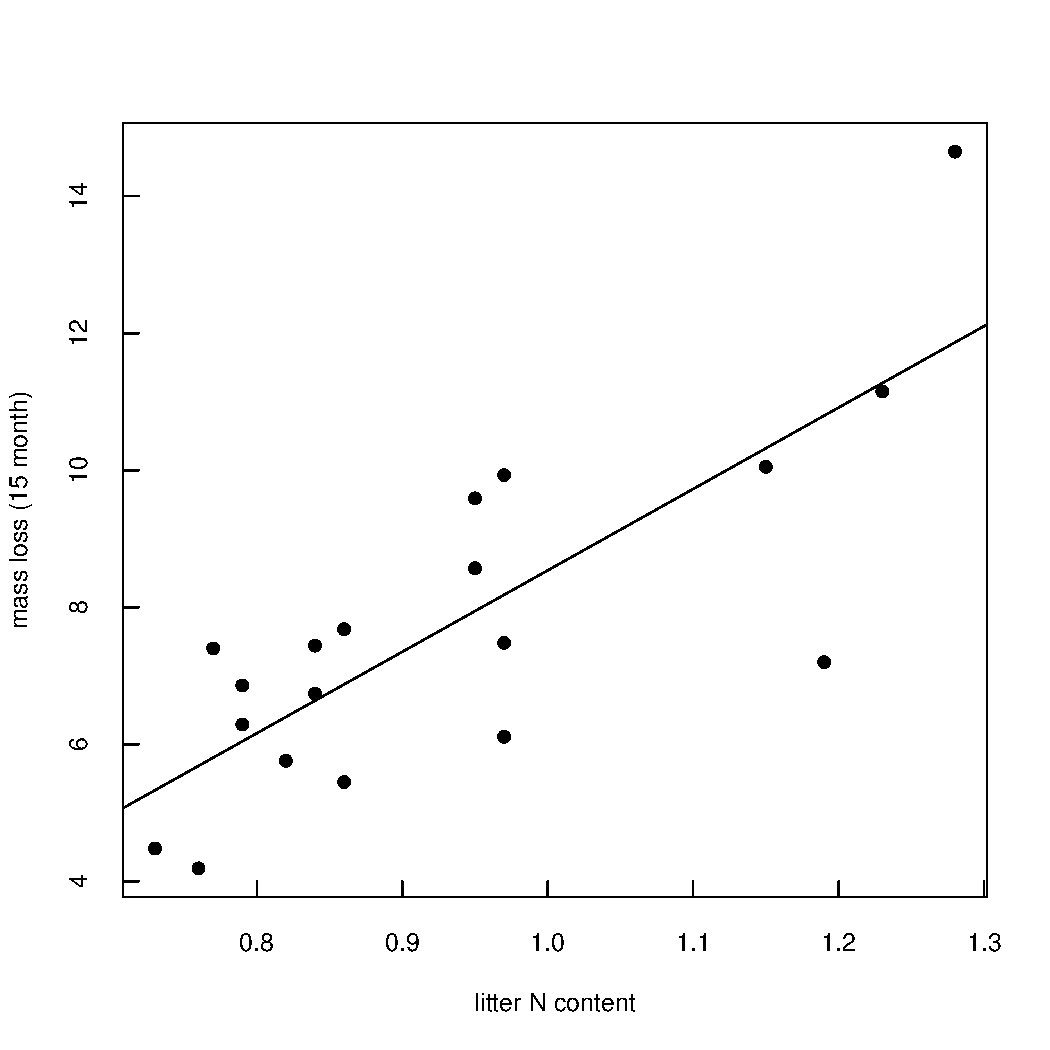
\includegraphics[width=8.3cm]{massloss_n_lit.pdf}
% \end{center}
% \label{fig:n_massloss}
% \caption{Litter mass loss after 15 month vs. litter N content. R= 0.795, p \textless .001}
% \end{figure}

% \newpage
% \begin{figure}[p]
% \vspace*{2mm}
% \begin{center}
% 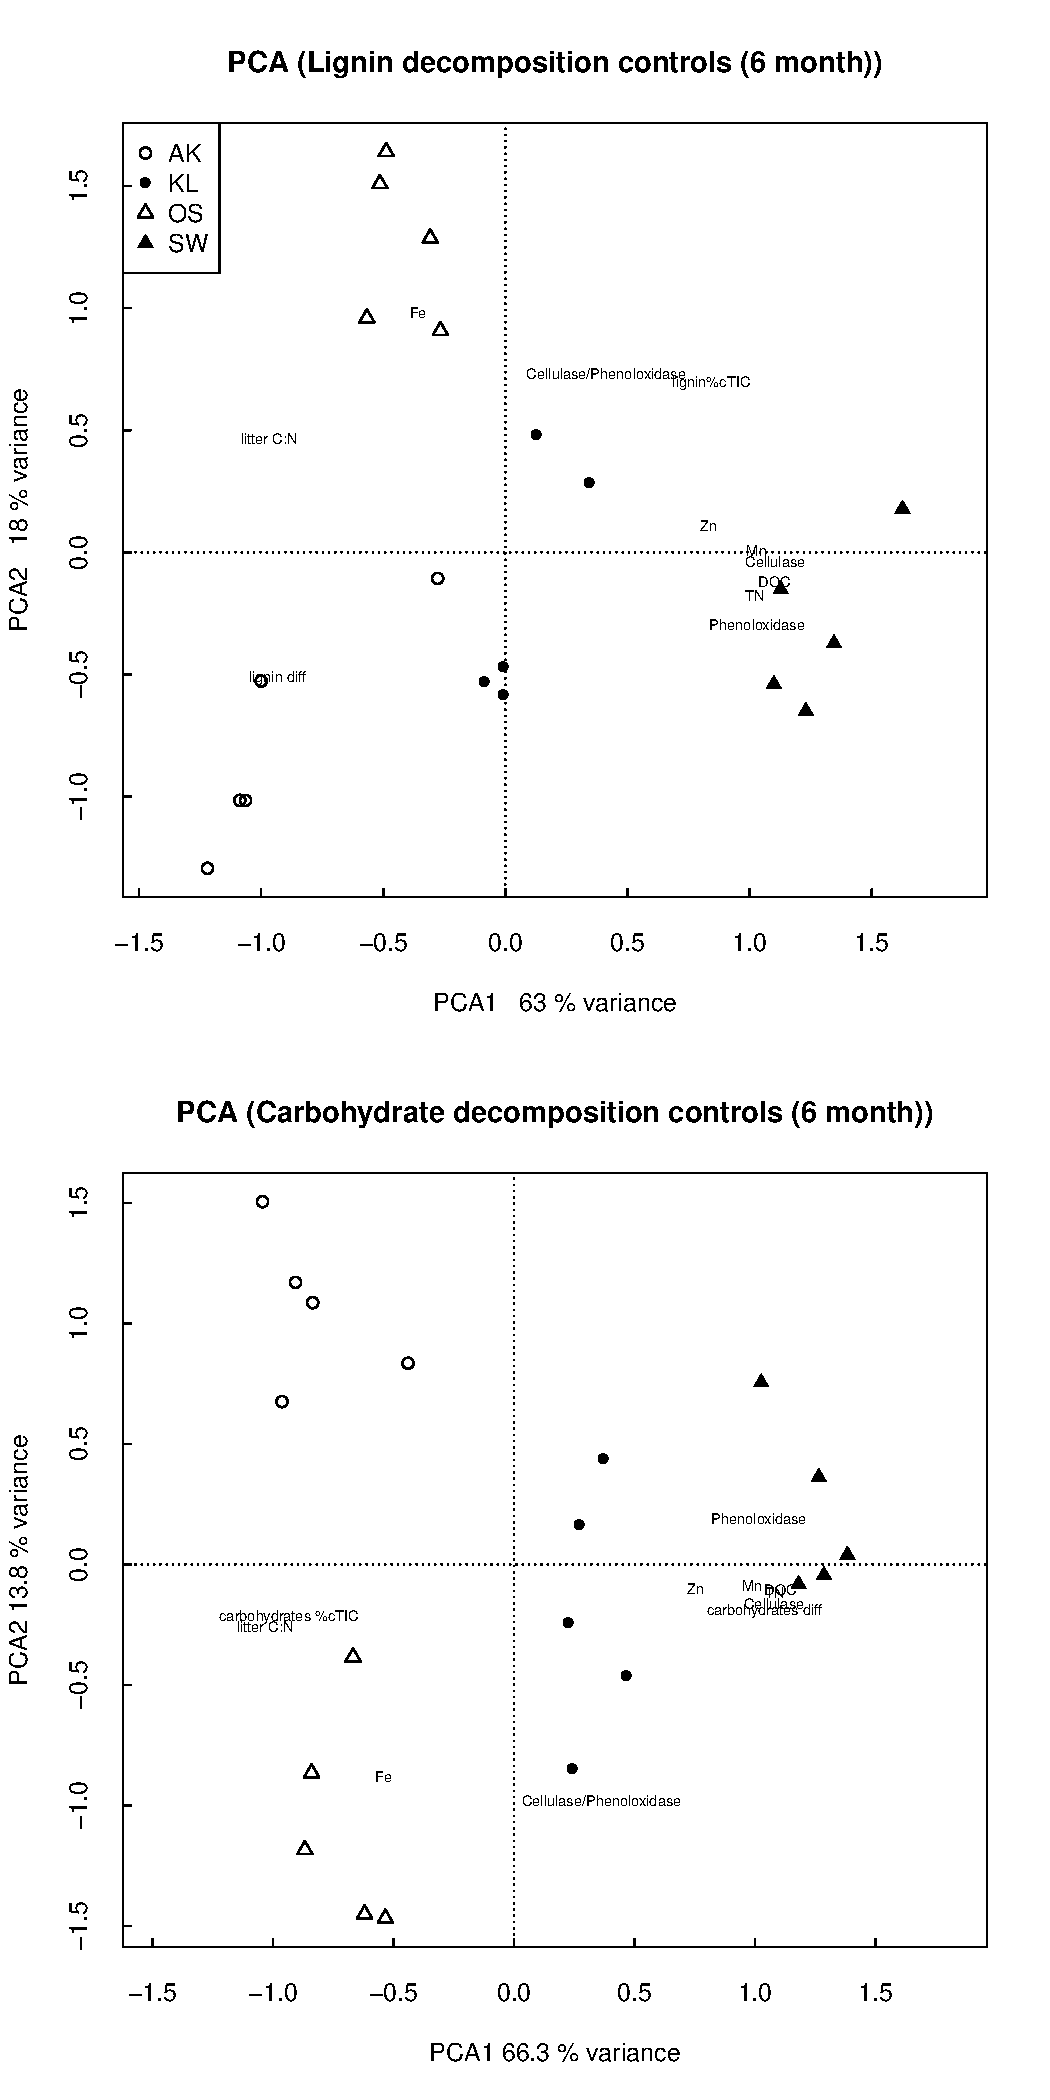
\includegraphics[width=8.3cm]{h3_decomp_contr.pdf}
% \end{center}
% \caption{Litter mass loss after 15 month vs. litter N content. R= 0.795, p \textless .001}
% \label{fig:h3_controls}
% \end{figure}

% \newpage
% \begin{figure*}[p]
% \vspace*{2mm}
% \begin{center}
% 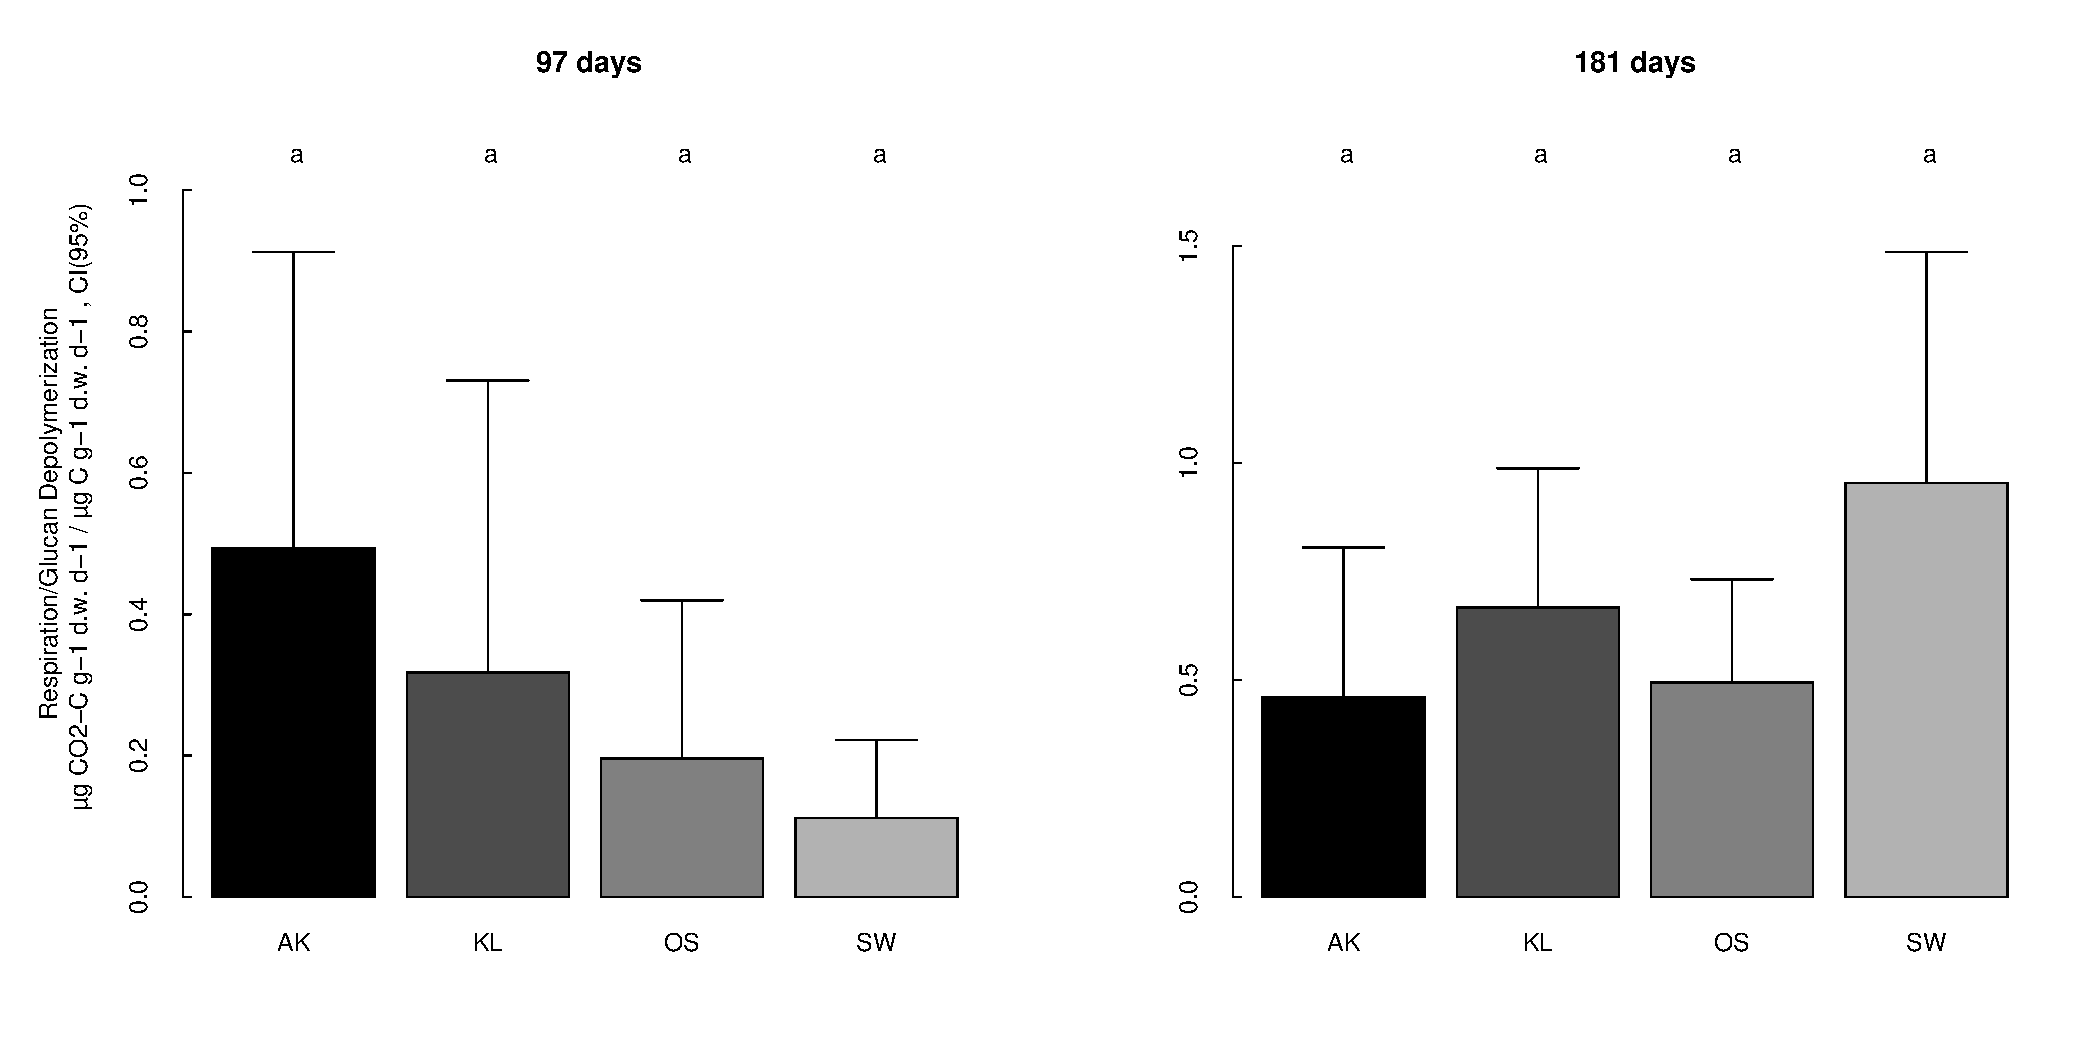
\includegraphics[width=12cm]{resp_glcdepoly_h23.pdf}
% \end{center}
% \caption{Quotient of respiration and glucan depolymerization. In AK microbial community respire significantly more non-glucose carbon after 2, but not after 6 month. Data from \cite{Leitner2011}}
% \label{fig:resp_depoly}
% \end{figure*}

\newpage
\begin{figure*}[p]
\vspace*{2mm}
% \begin{center}
% 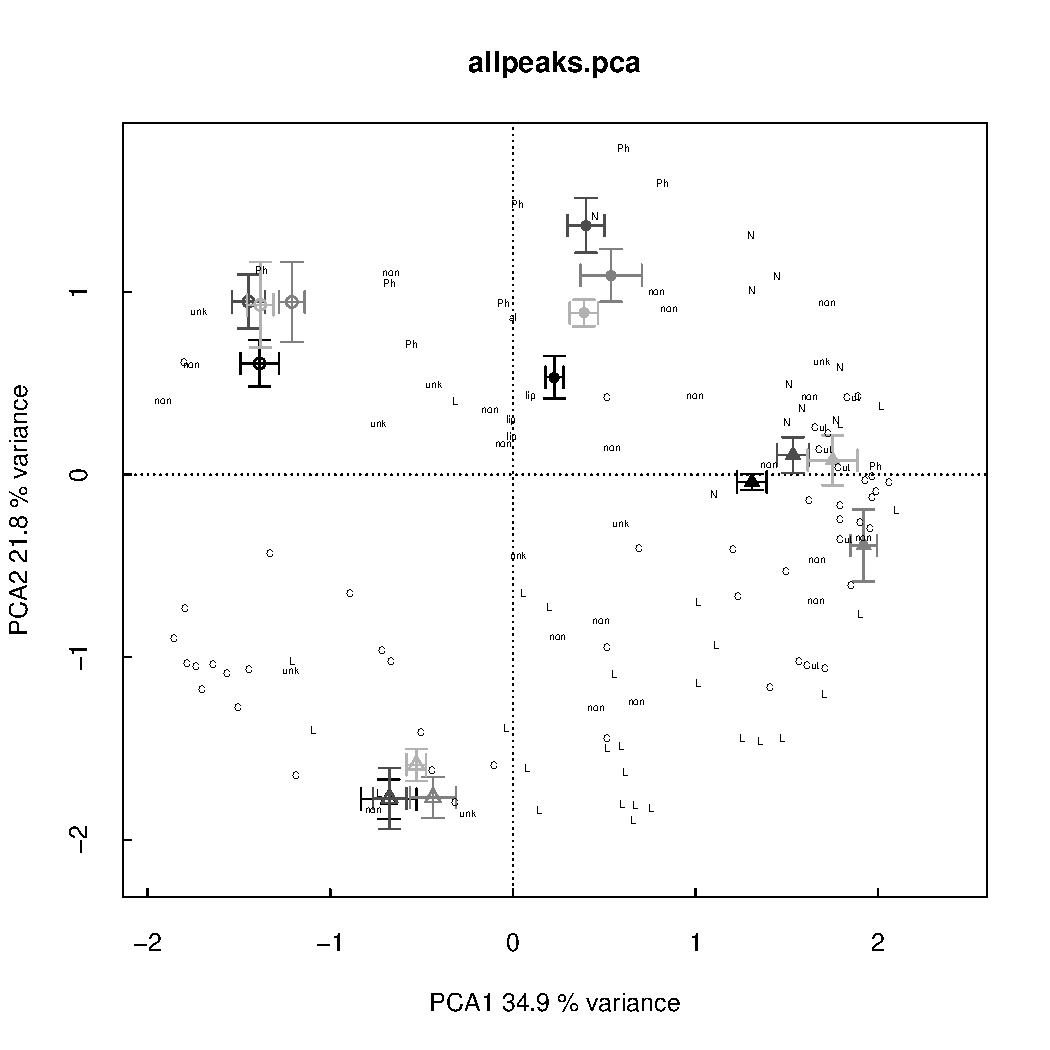
\includegraphics[width=15cm]{allpeaks_PCA12.pdf}
% %\includegraphics[width=10cm]{allpeaks_allharvests_PCA34.pdf}
% \end{center}
\caption{PCA of relative abundances of all 125 pyrolysis products. Open circles - AK, full circles - KL, open triangles - OS, full triangles - SW. black to light grey: harvest 0, 2, 3, and 4. Errorbars indicate 1 SE (n=4-5).}
\label{fig:pca.all}
\end{figure*}


 \newpage
 \begin{figure*}[p]
 \vspace*{2mm}
 %\begin{center}
 %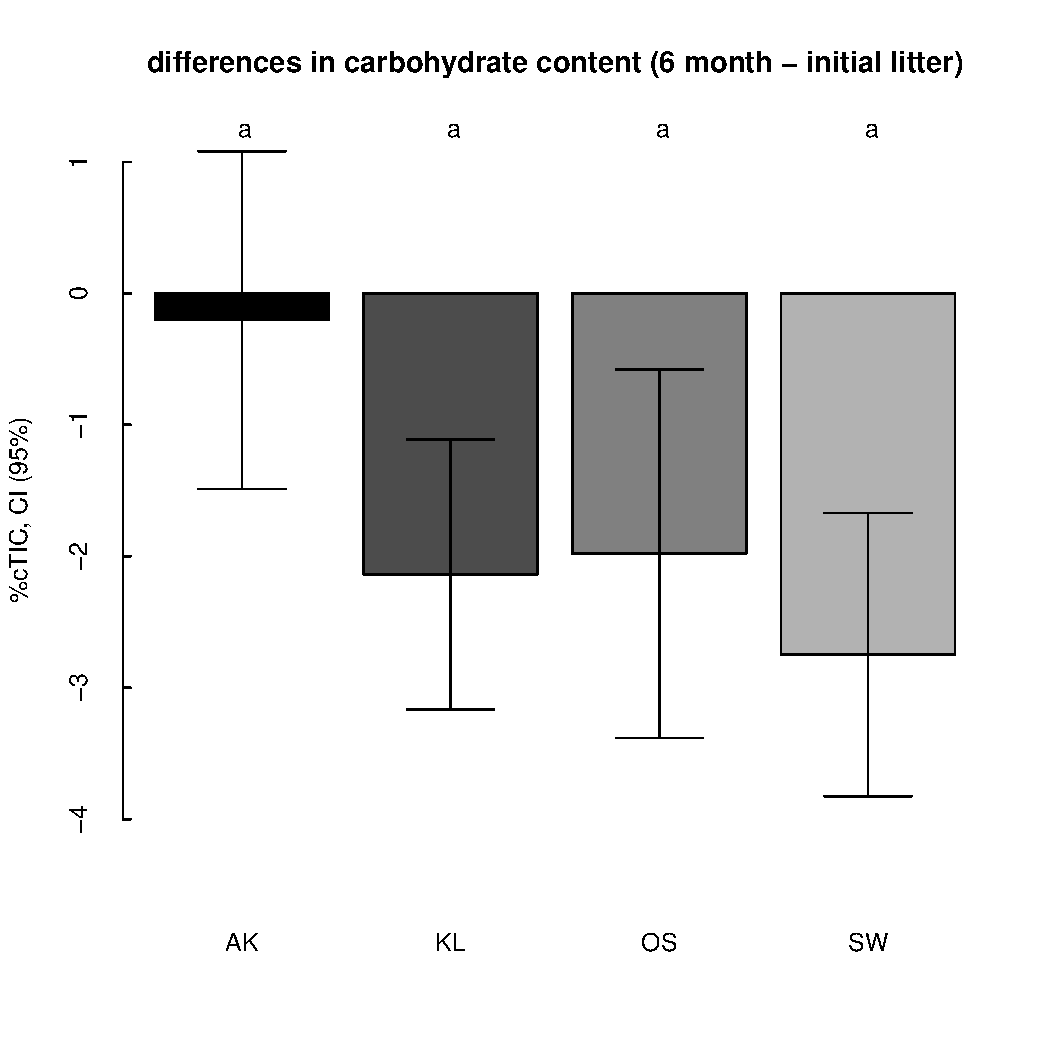
\includegraphics[width=8.3cm]{carb_differences_h3h0.pdf}
 %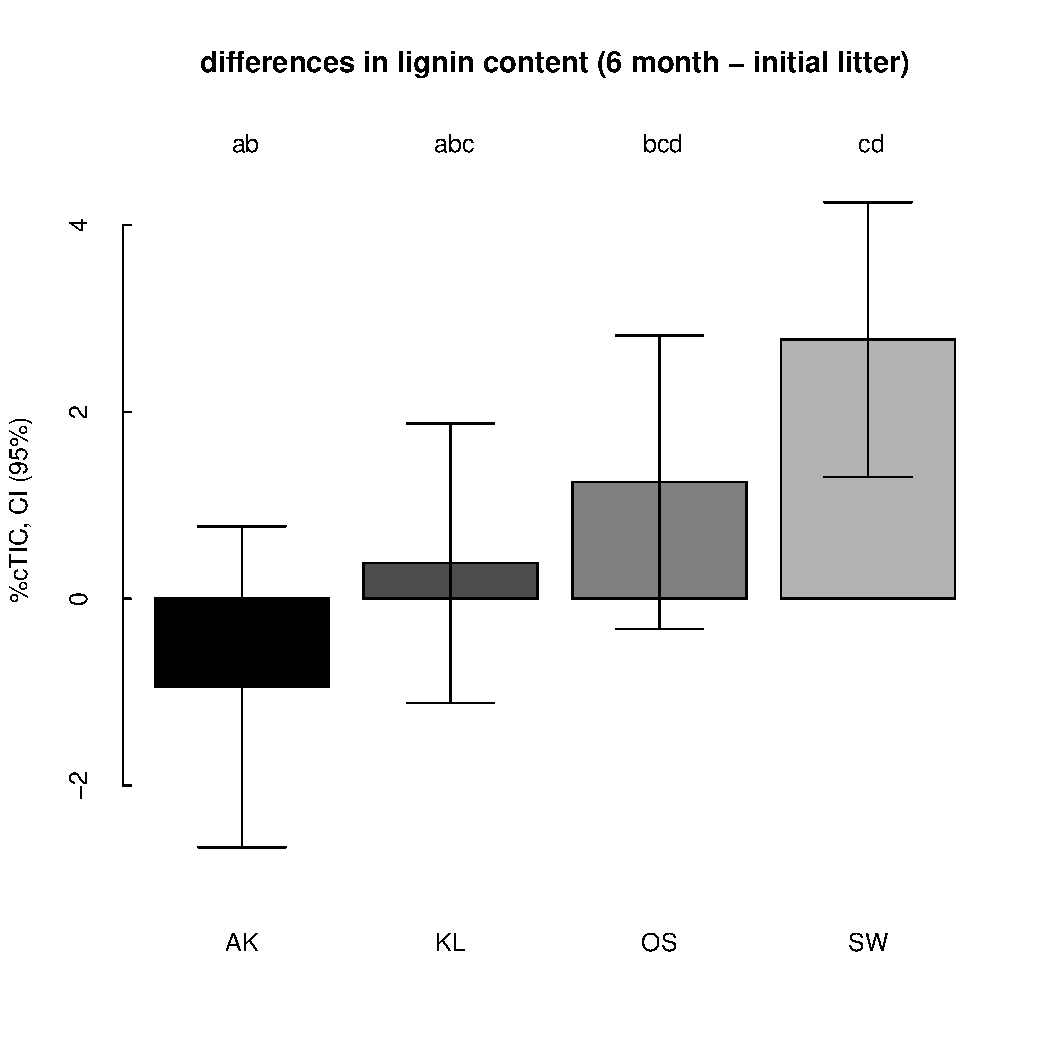
\includegraphics[width=8.3cm]{lig_differences_h3h0.pdf}
 %\end{center}
 \caption{Difference in \% cTIC (sum of lig markers). error bars indicate 95\% confidence intervall.}
 \label{fig:car_lig_6month}
 \end{figure*}


\newpage
\begin{figure*}[p]
\vspace*{2mm}
% \begin{center}
% 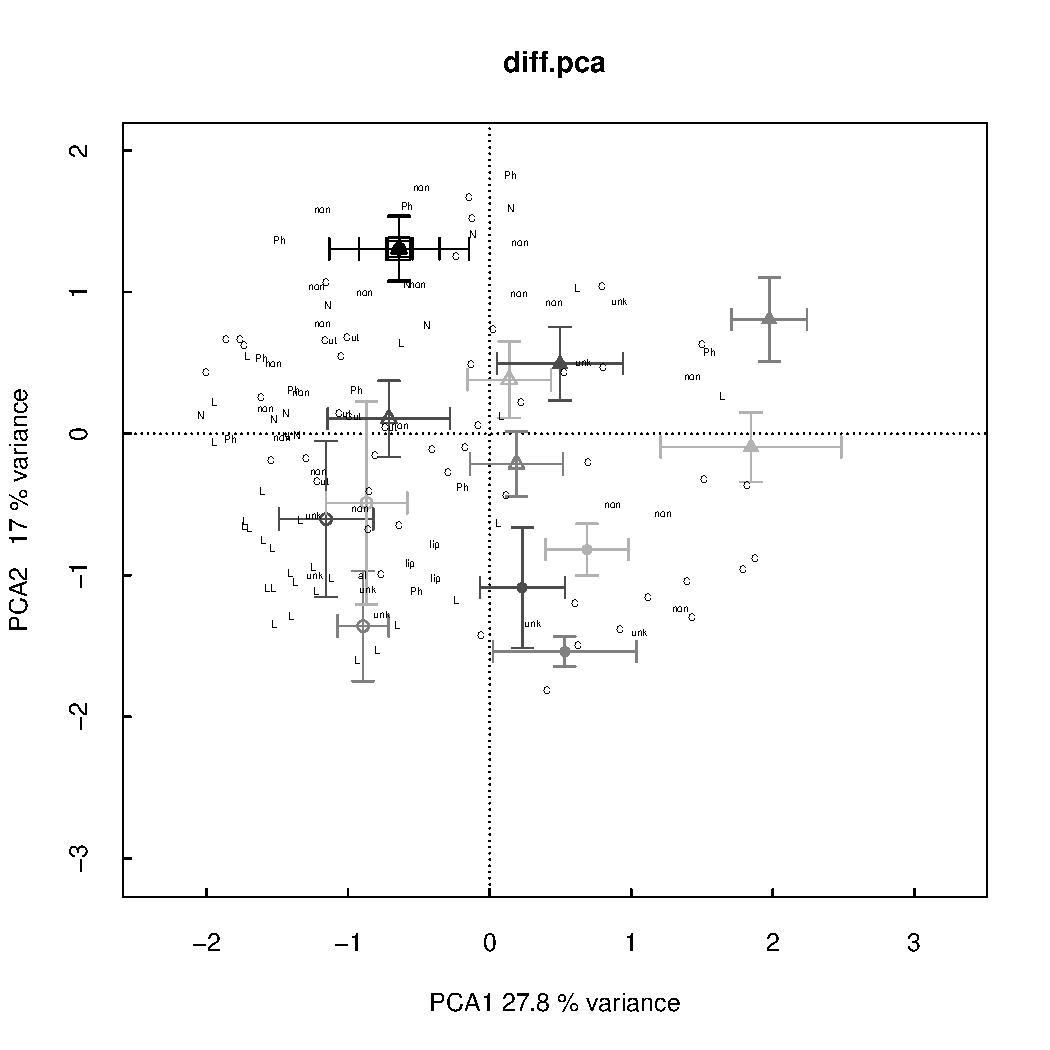
\includegraphics[width=15cm]{allpeaks_diffs_PCA12.pdf}
% \end{center}
\caption{PCA of relative abundances of 125 products minus the mean relative abundance of the product in initial litter of the corresponding litter type. Open circles - AK, full circles - KL, open triangles - OS, full triangles - SW. black to light grey: harvest 0, 2, 3, and 4. Errorbars indicate 1 SE (n=4-5). Decompositino trends follow PCA1 for SW and PCA2 for AK. KL and OS show mixed trends.}
\label{fig:pca.dif}
\end{figure*}


\newpage
\begin{figure*}[p]
\caption{Development of the LCI (Lignin:(Lignin+Carbohydrates) and Lignin:N ratio}
\label{fig:lci}
\end{figure*}


\newpage
\begin{figure*}[p]
\vspace*{2mm}
% \begin{center}
% 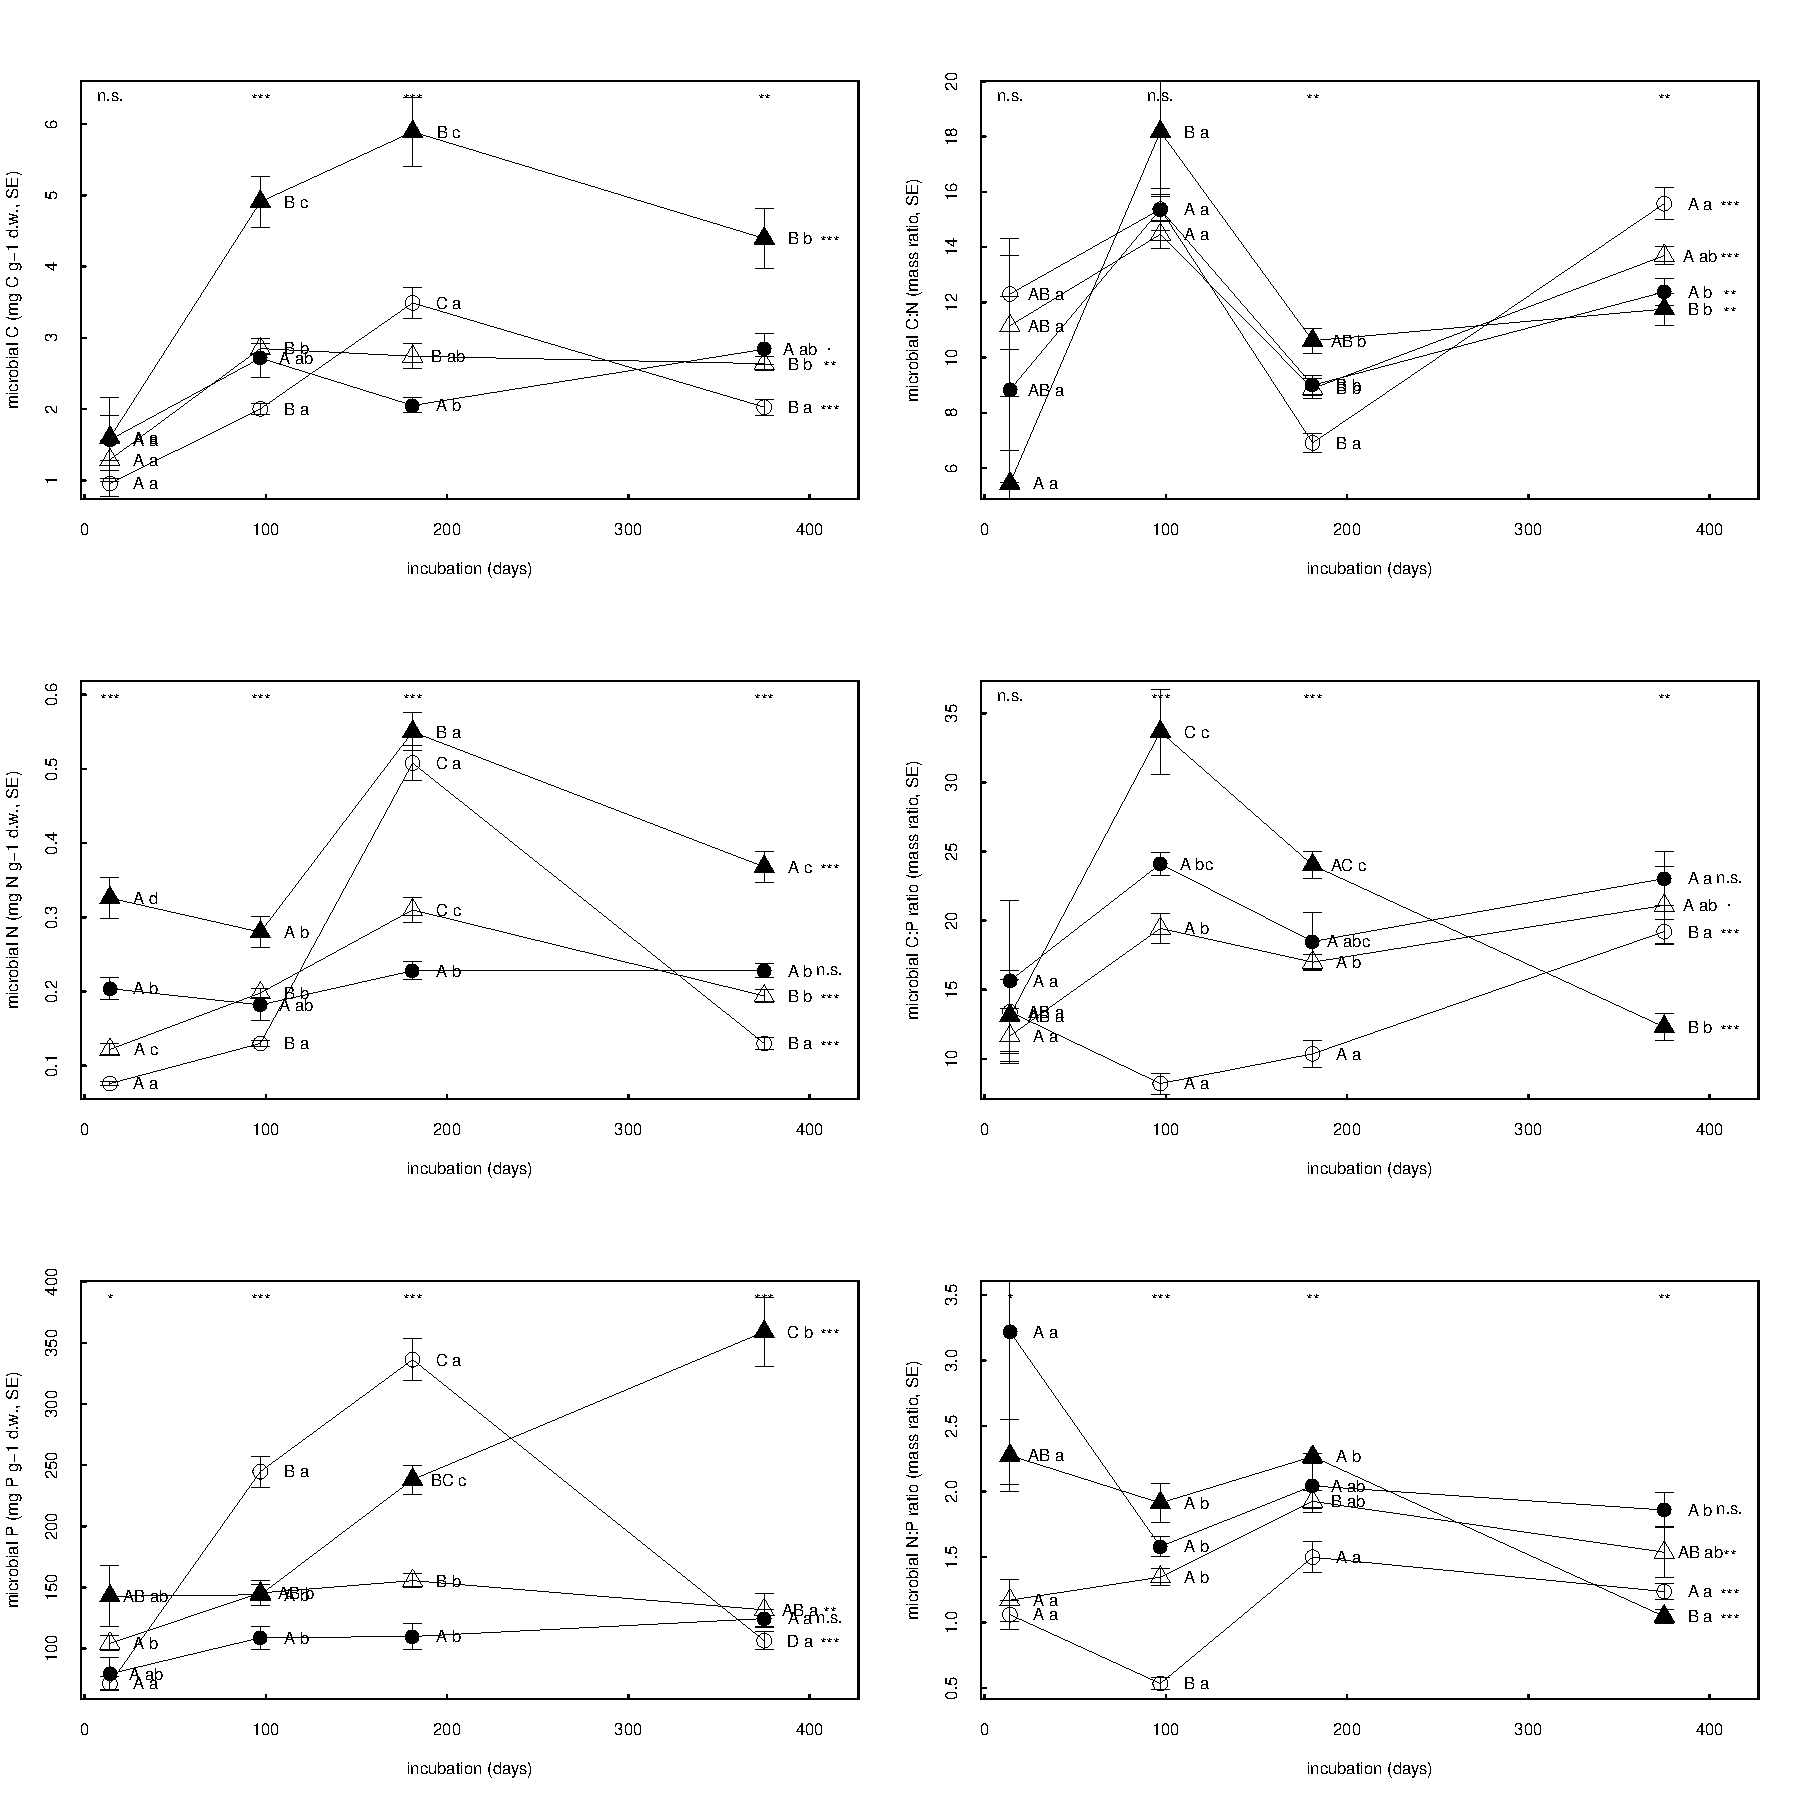
\includegraphics[width=15cm]{microbialbiomass.pdf}
% \end{center}
\caption{Microbial C, N and P content and their ratios.}
\label{fig:bm}
\end{figure*}

\newpage
\begin{figure*}[p]
\vspace*{2mm}
% \begin{center}
% 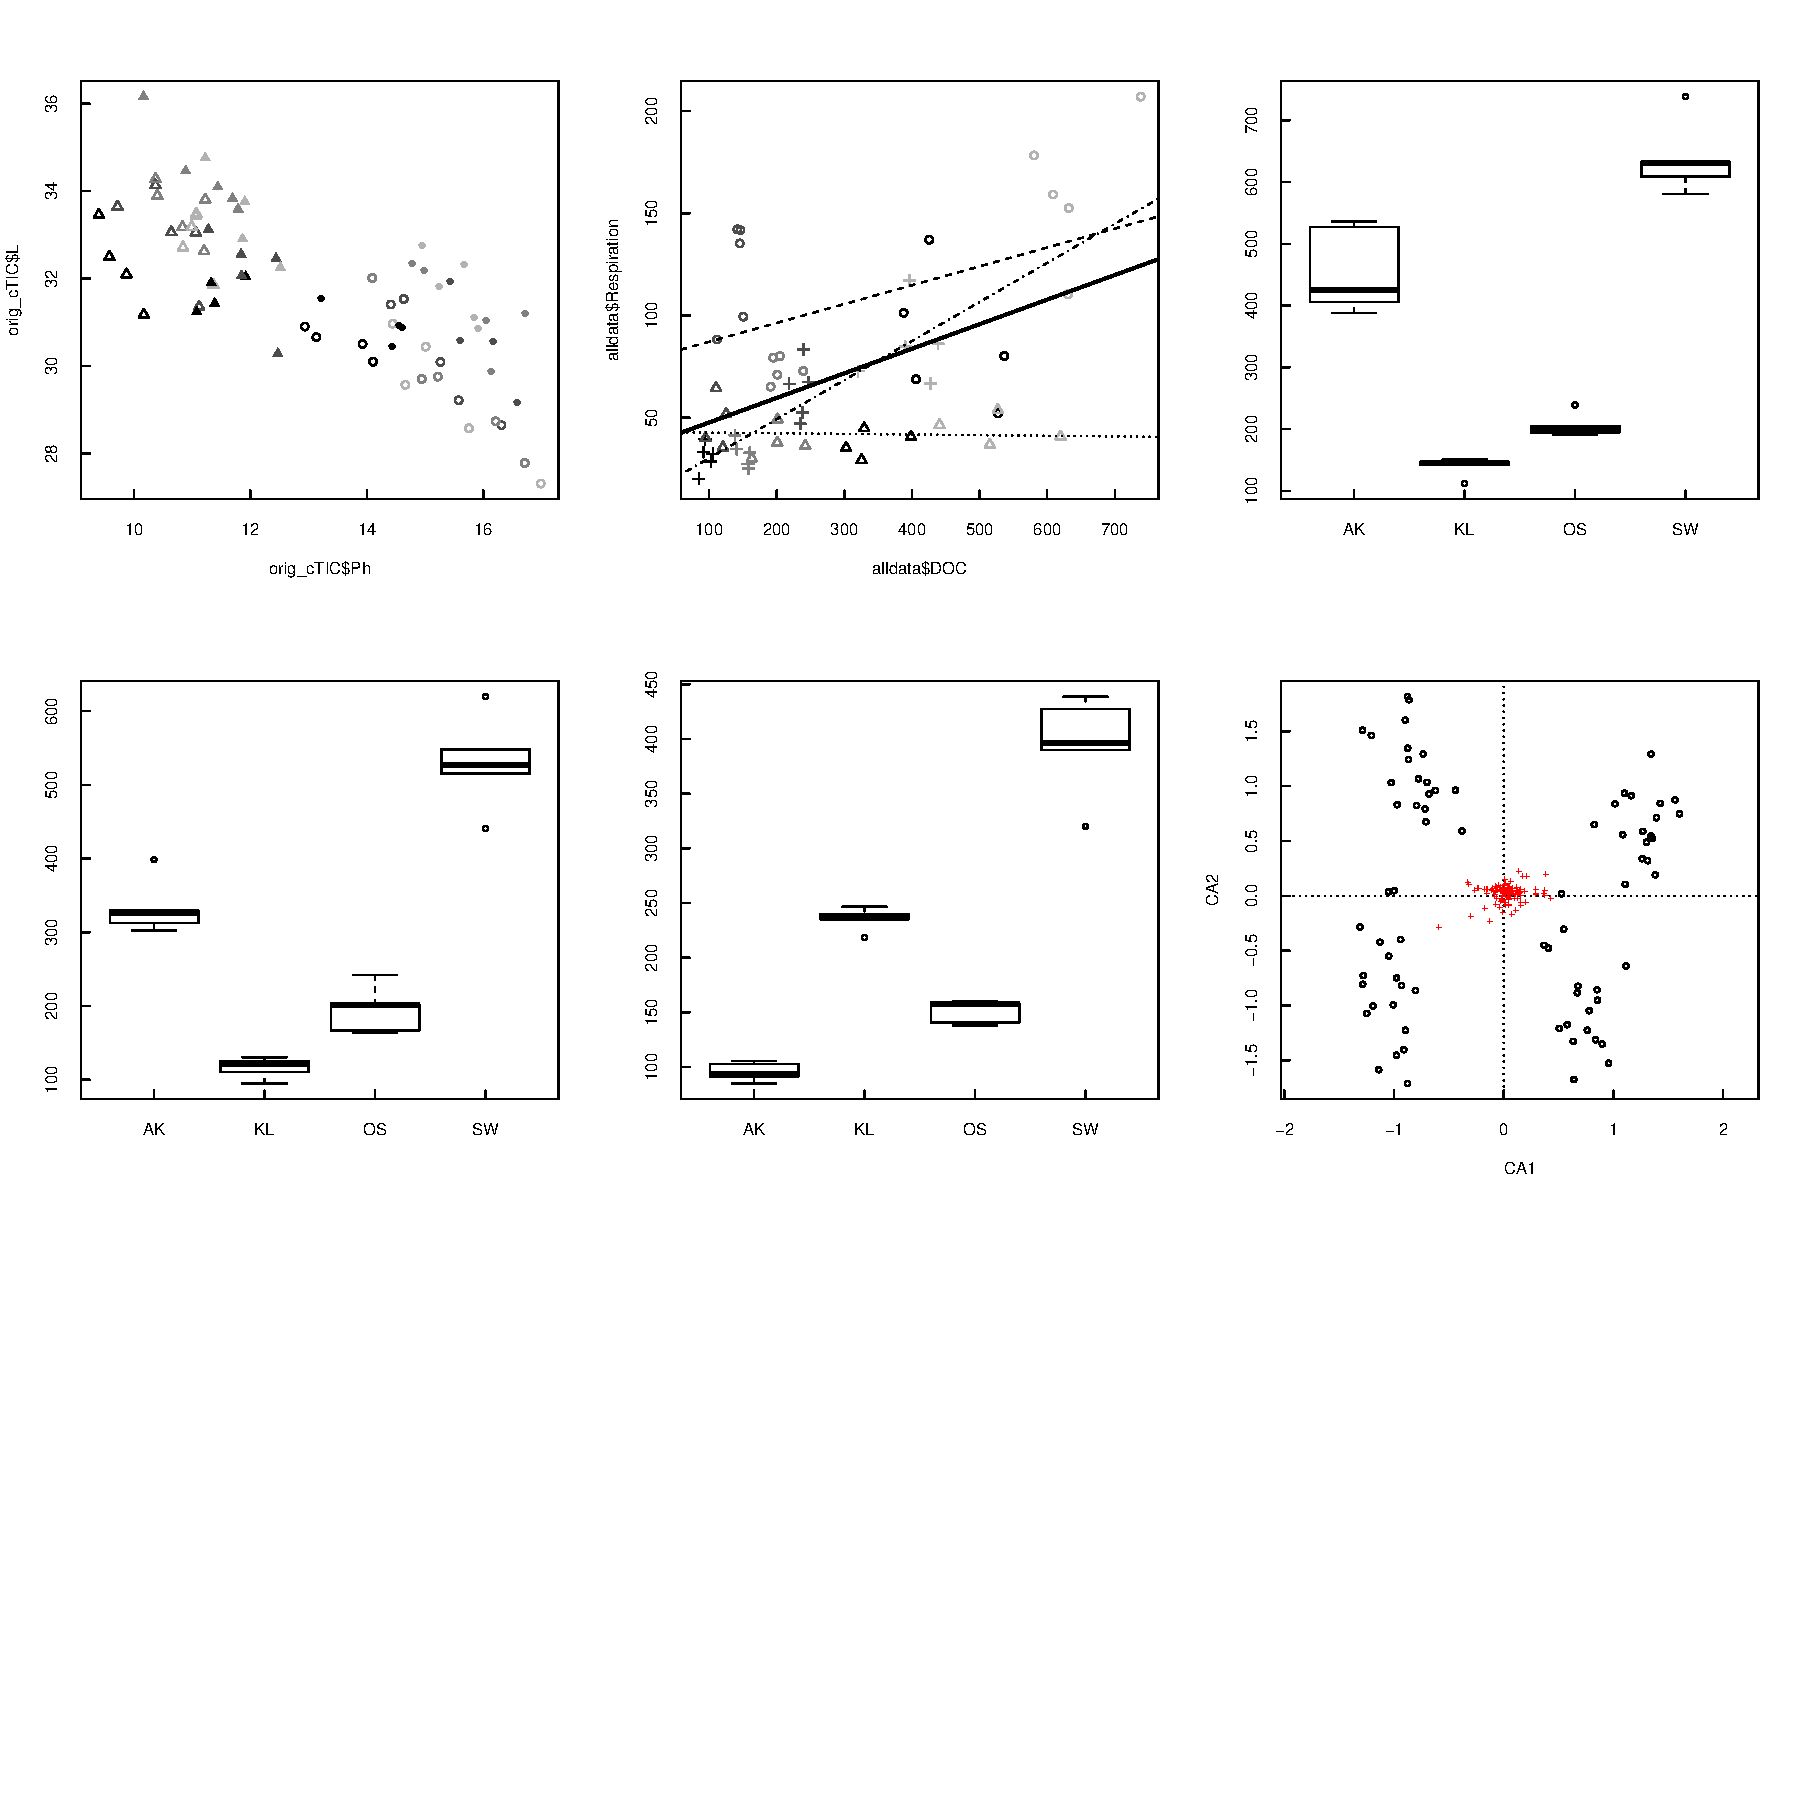
\includegraphics[width=12cm]{enzymes_barplots.pdf}
% \end{center}
\caption{Potential activities of cellulase, phenoloxidase and perodase.}
\label{fig:enz}
\end{figure*}

\newpage
\begin{figure*}[p]
\vspace*{2mm}
% \begin{center}
% 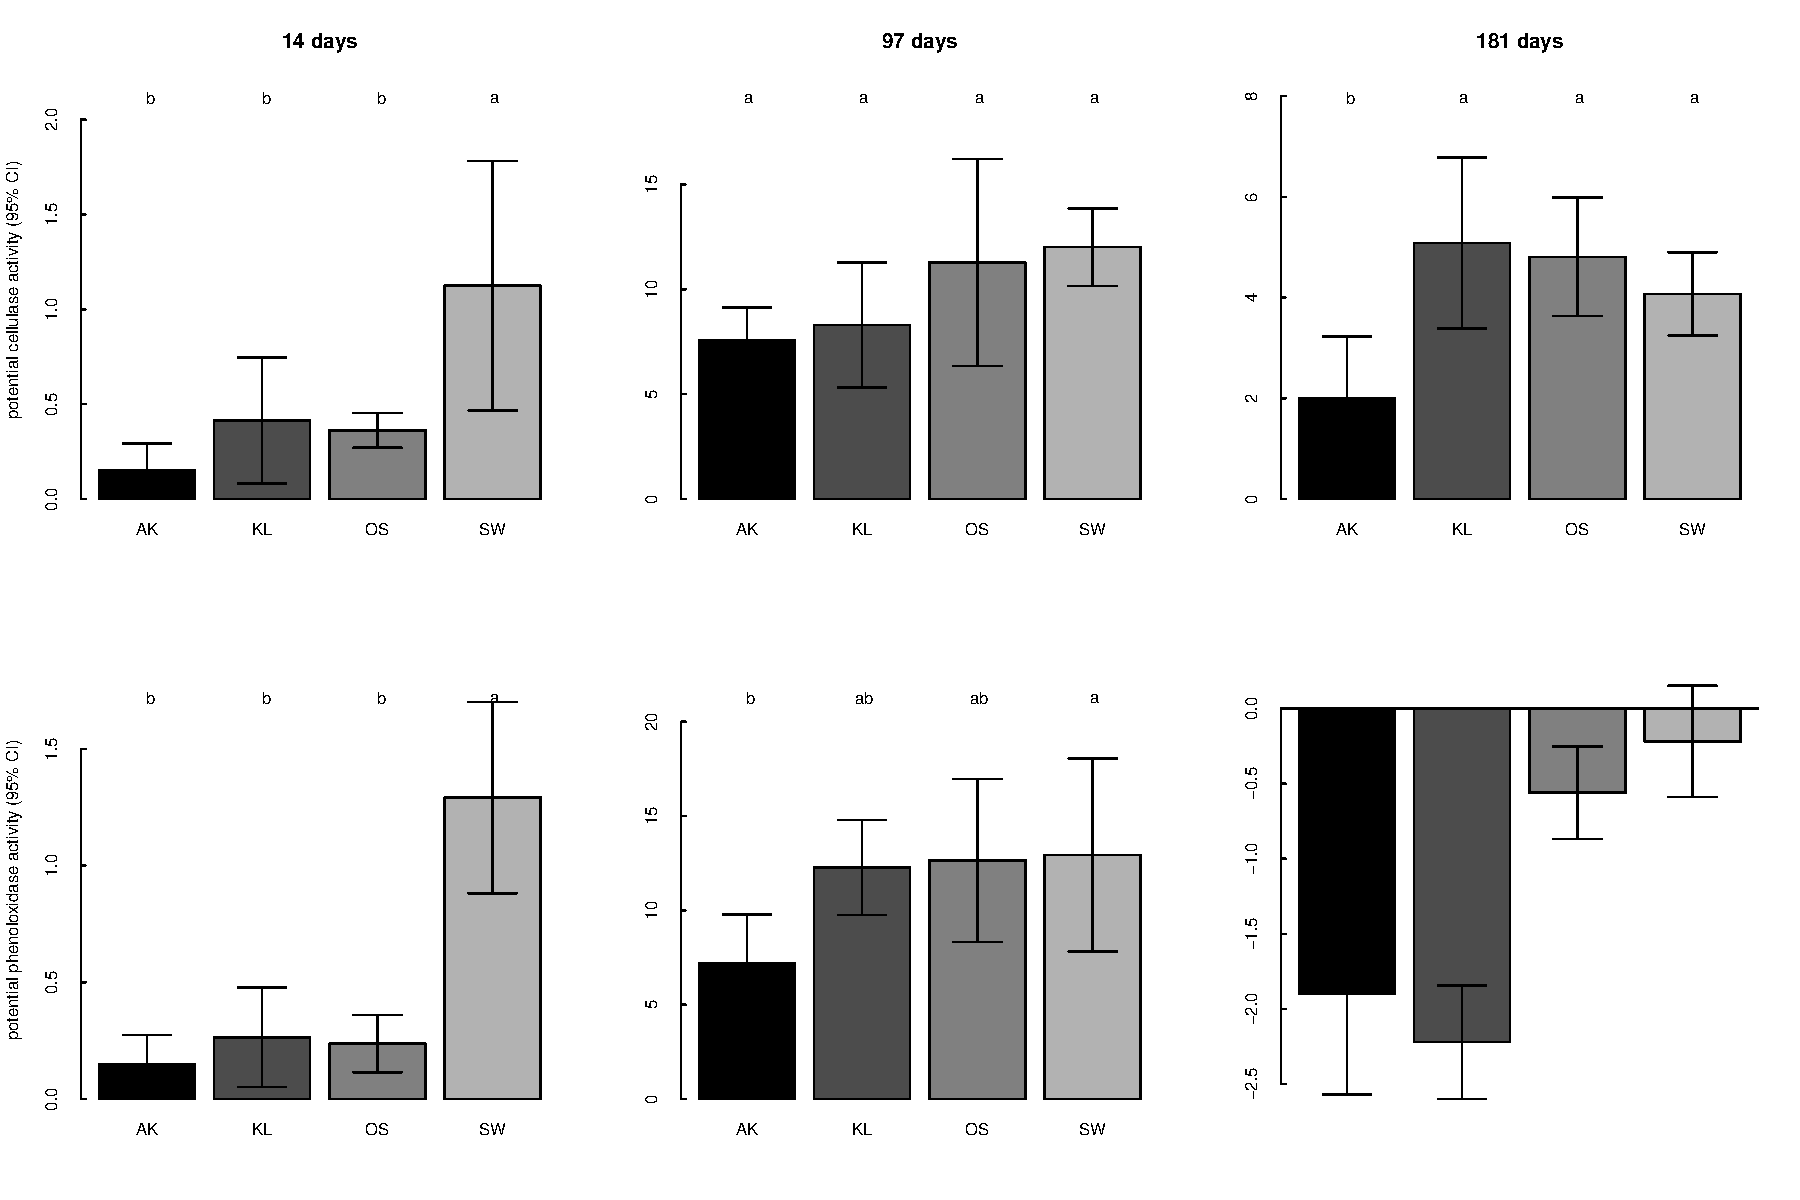
\includegraphics[width=12cm]{enzyme_ratio_barplots.pdf}
% \end{center}
\caption{Ratio between cellulase and two oxidative enzymes (phenolxydase and peroxydase). The two ratios are strongly correlated, oxidative enzymes are higher in AK than in other litter types.}
\label{fig:enz_ratio}
\end{figure*}

\newpage
\begin{figure*}[p]
\vspace*{2mm}
%   \begin{center}
% 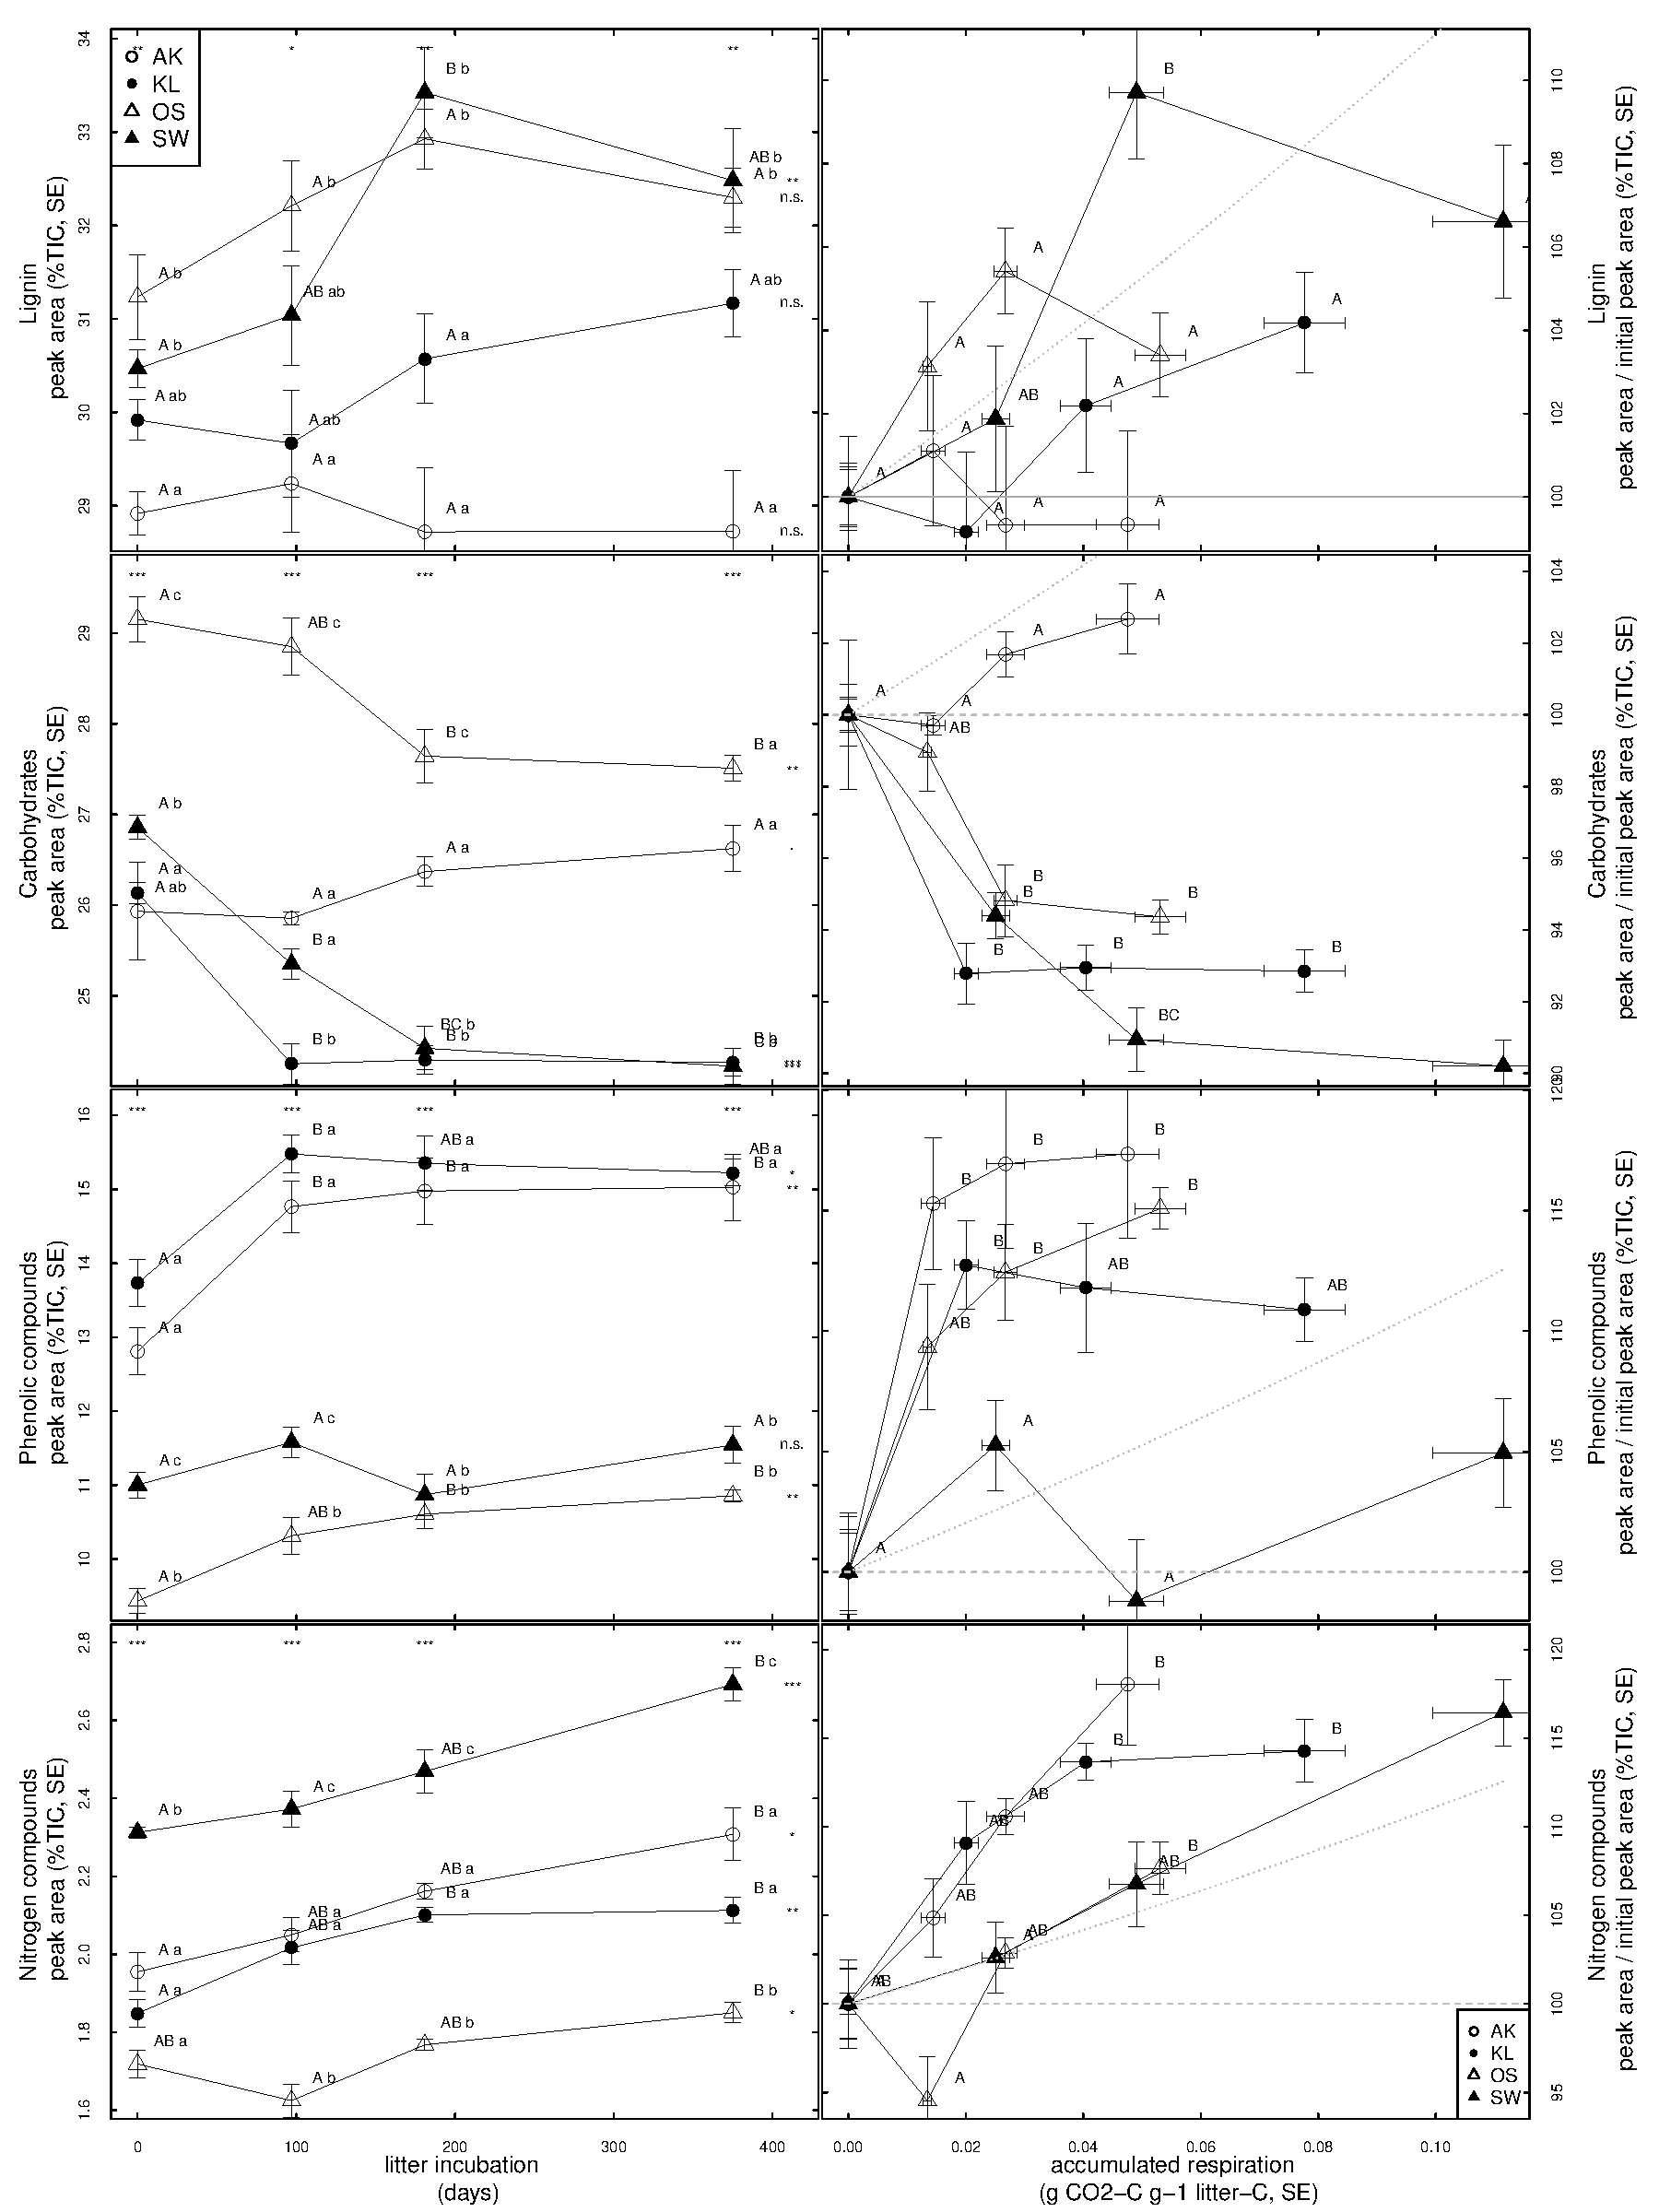
\includegraphics[width=15cm]{timeseries_orig.pdf}
% %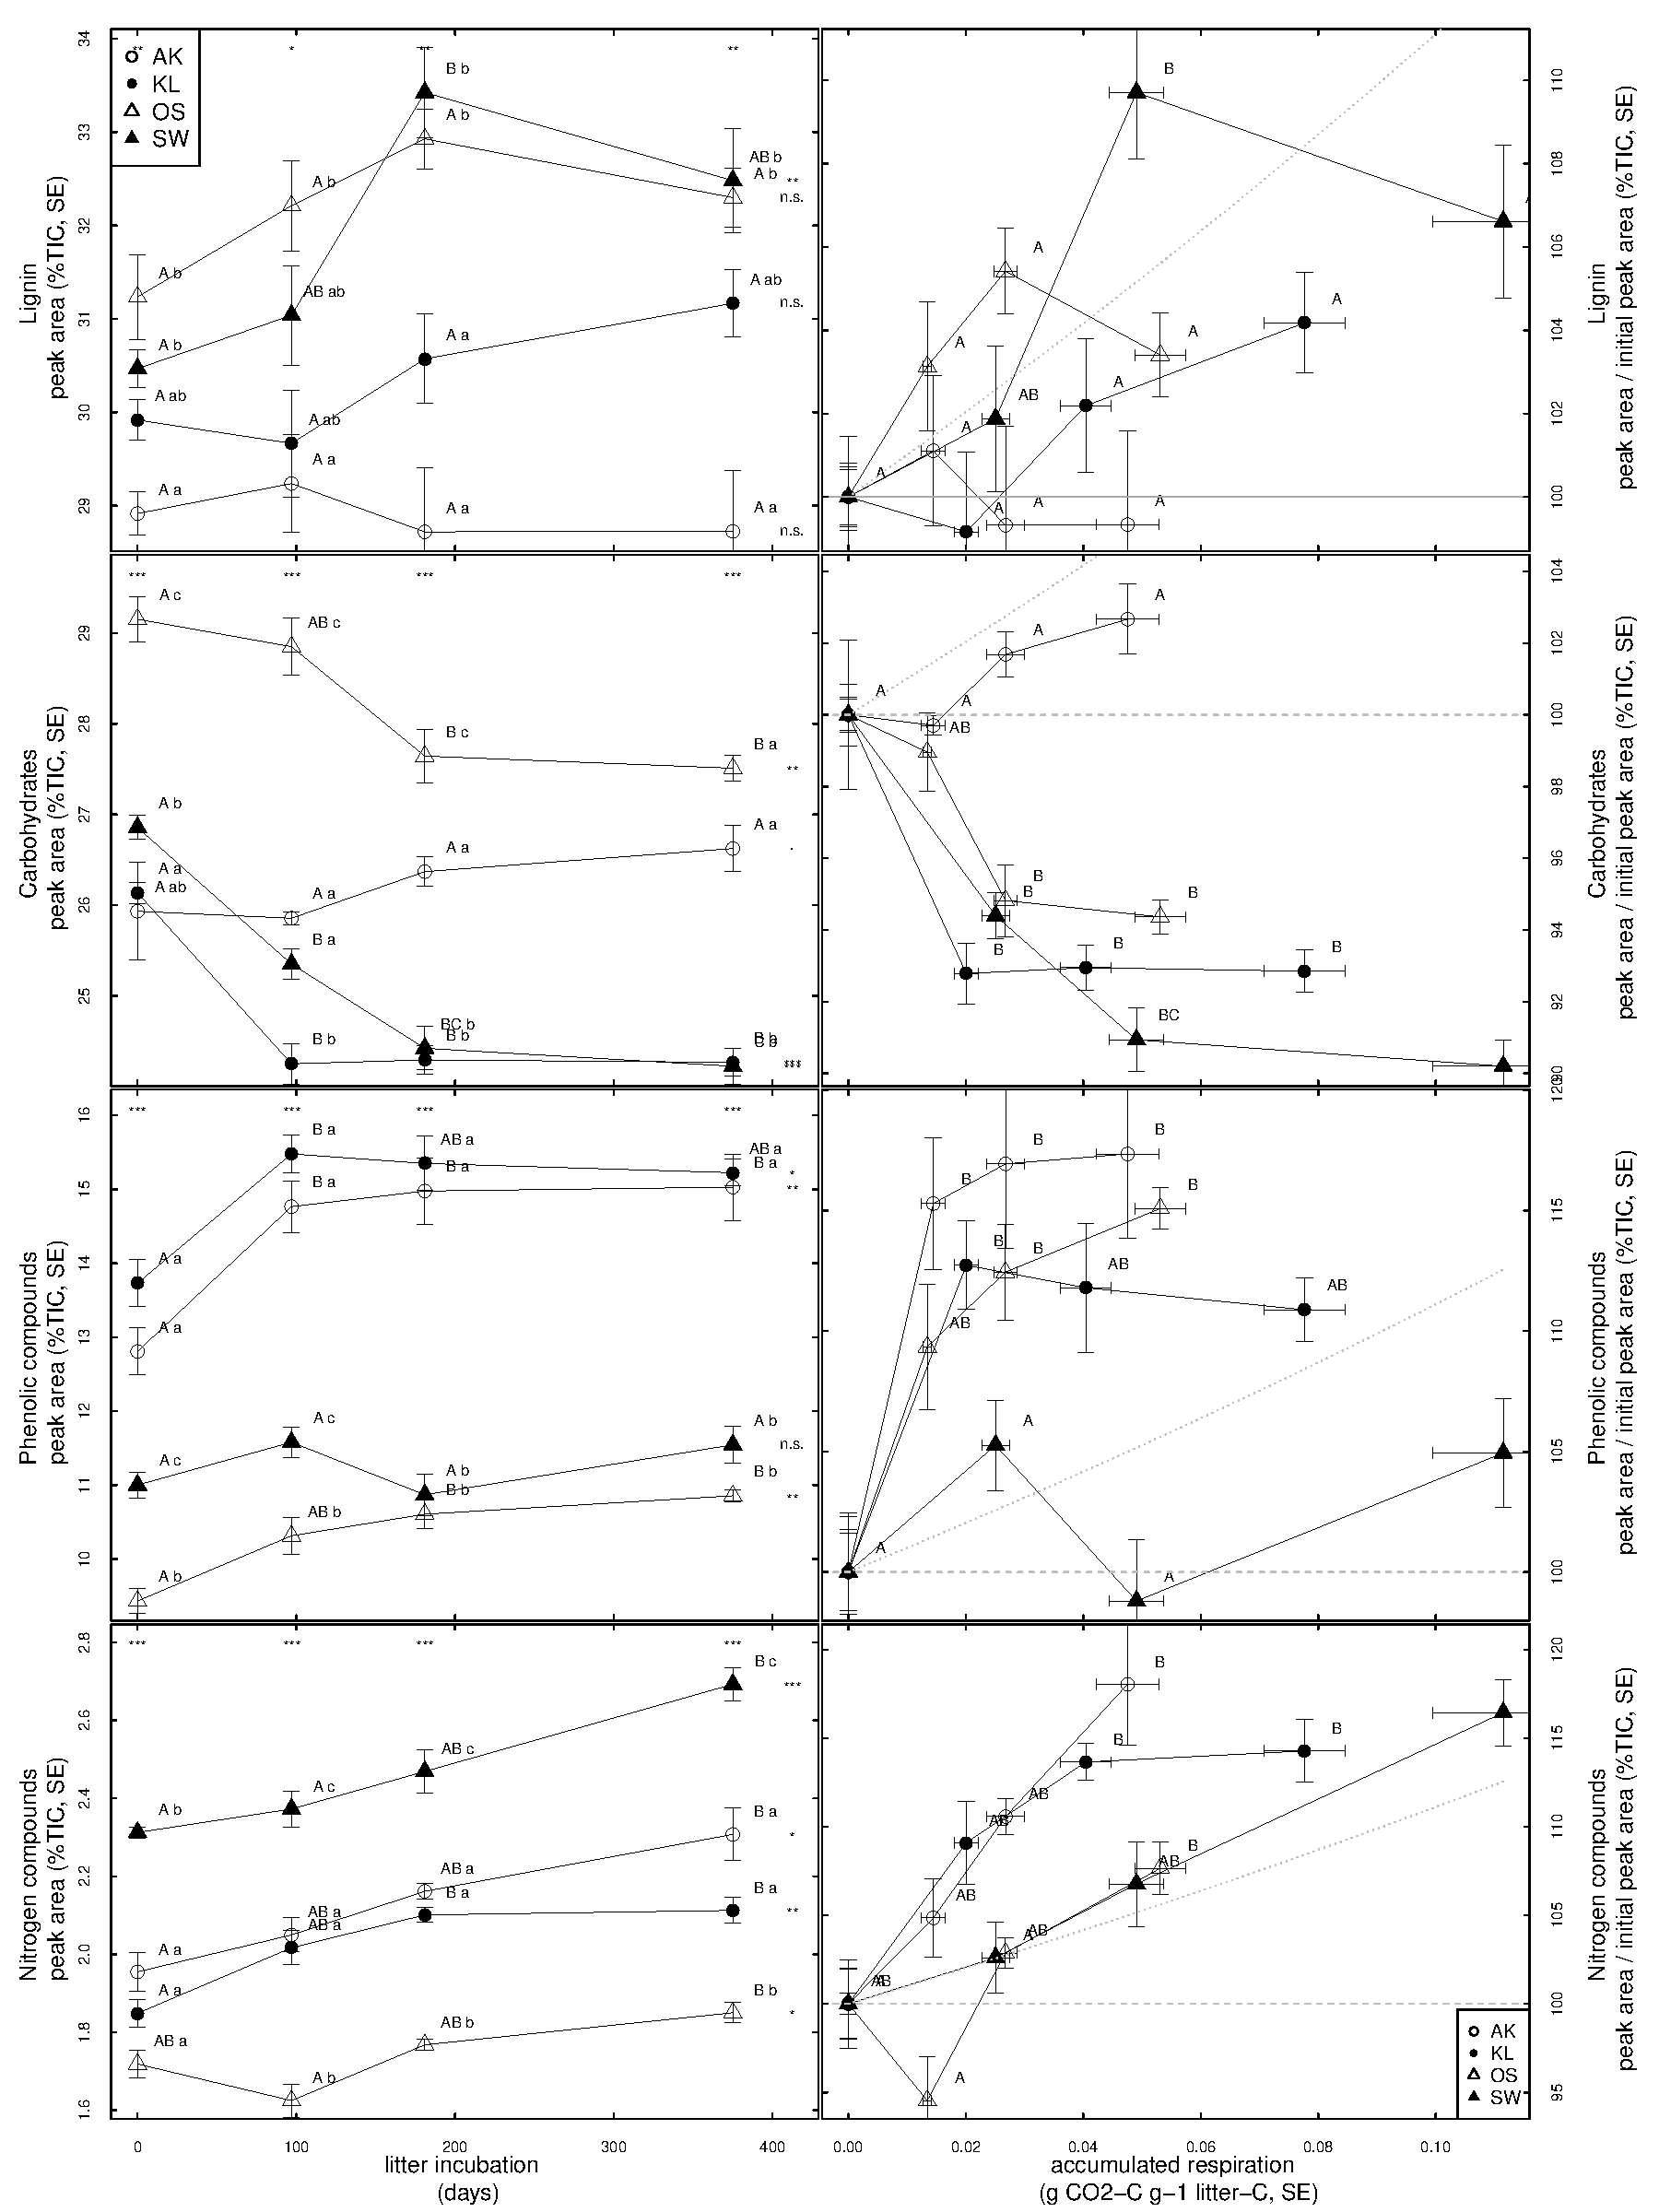
\includegraphics[width=17cm]{timeseries_orig.pdf}
% \end{center}
\caption{Decomposition dynamics of HMW compound classes}
\label{fig:timeseries}
\end{figure*}

\newpage 
\begin{figure*}[p]
\vspace*{2mm}
%   \begin{center}
% 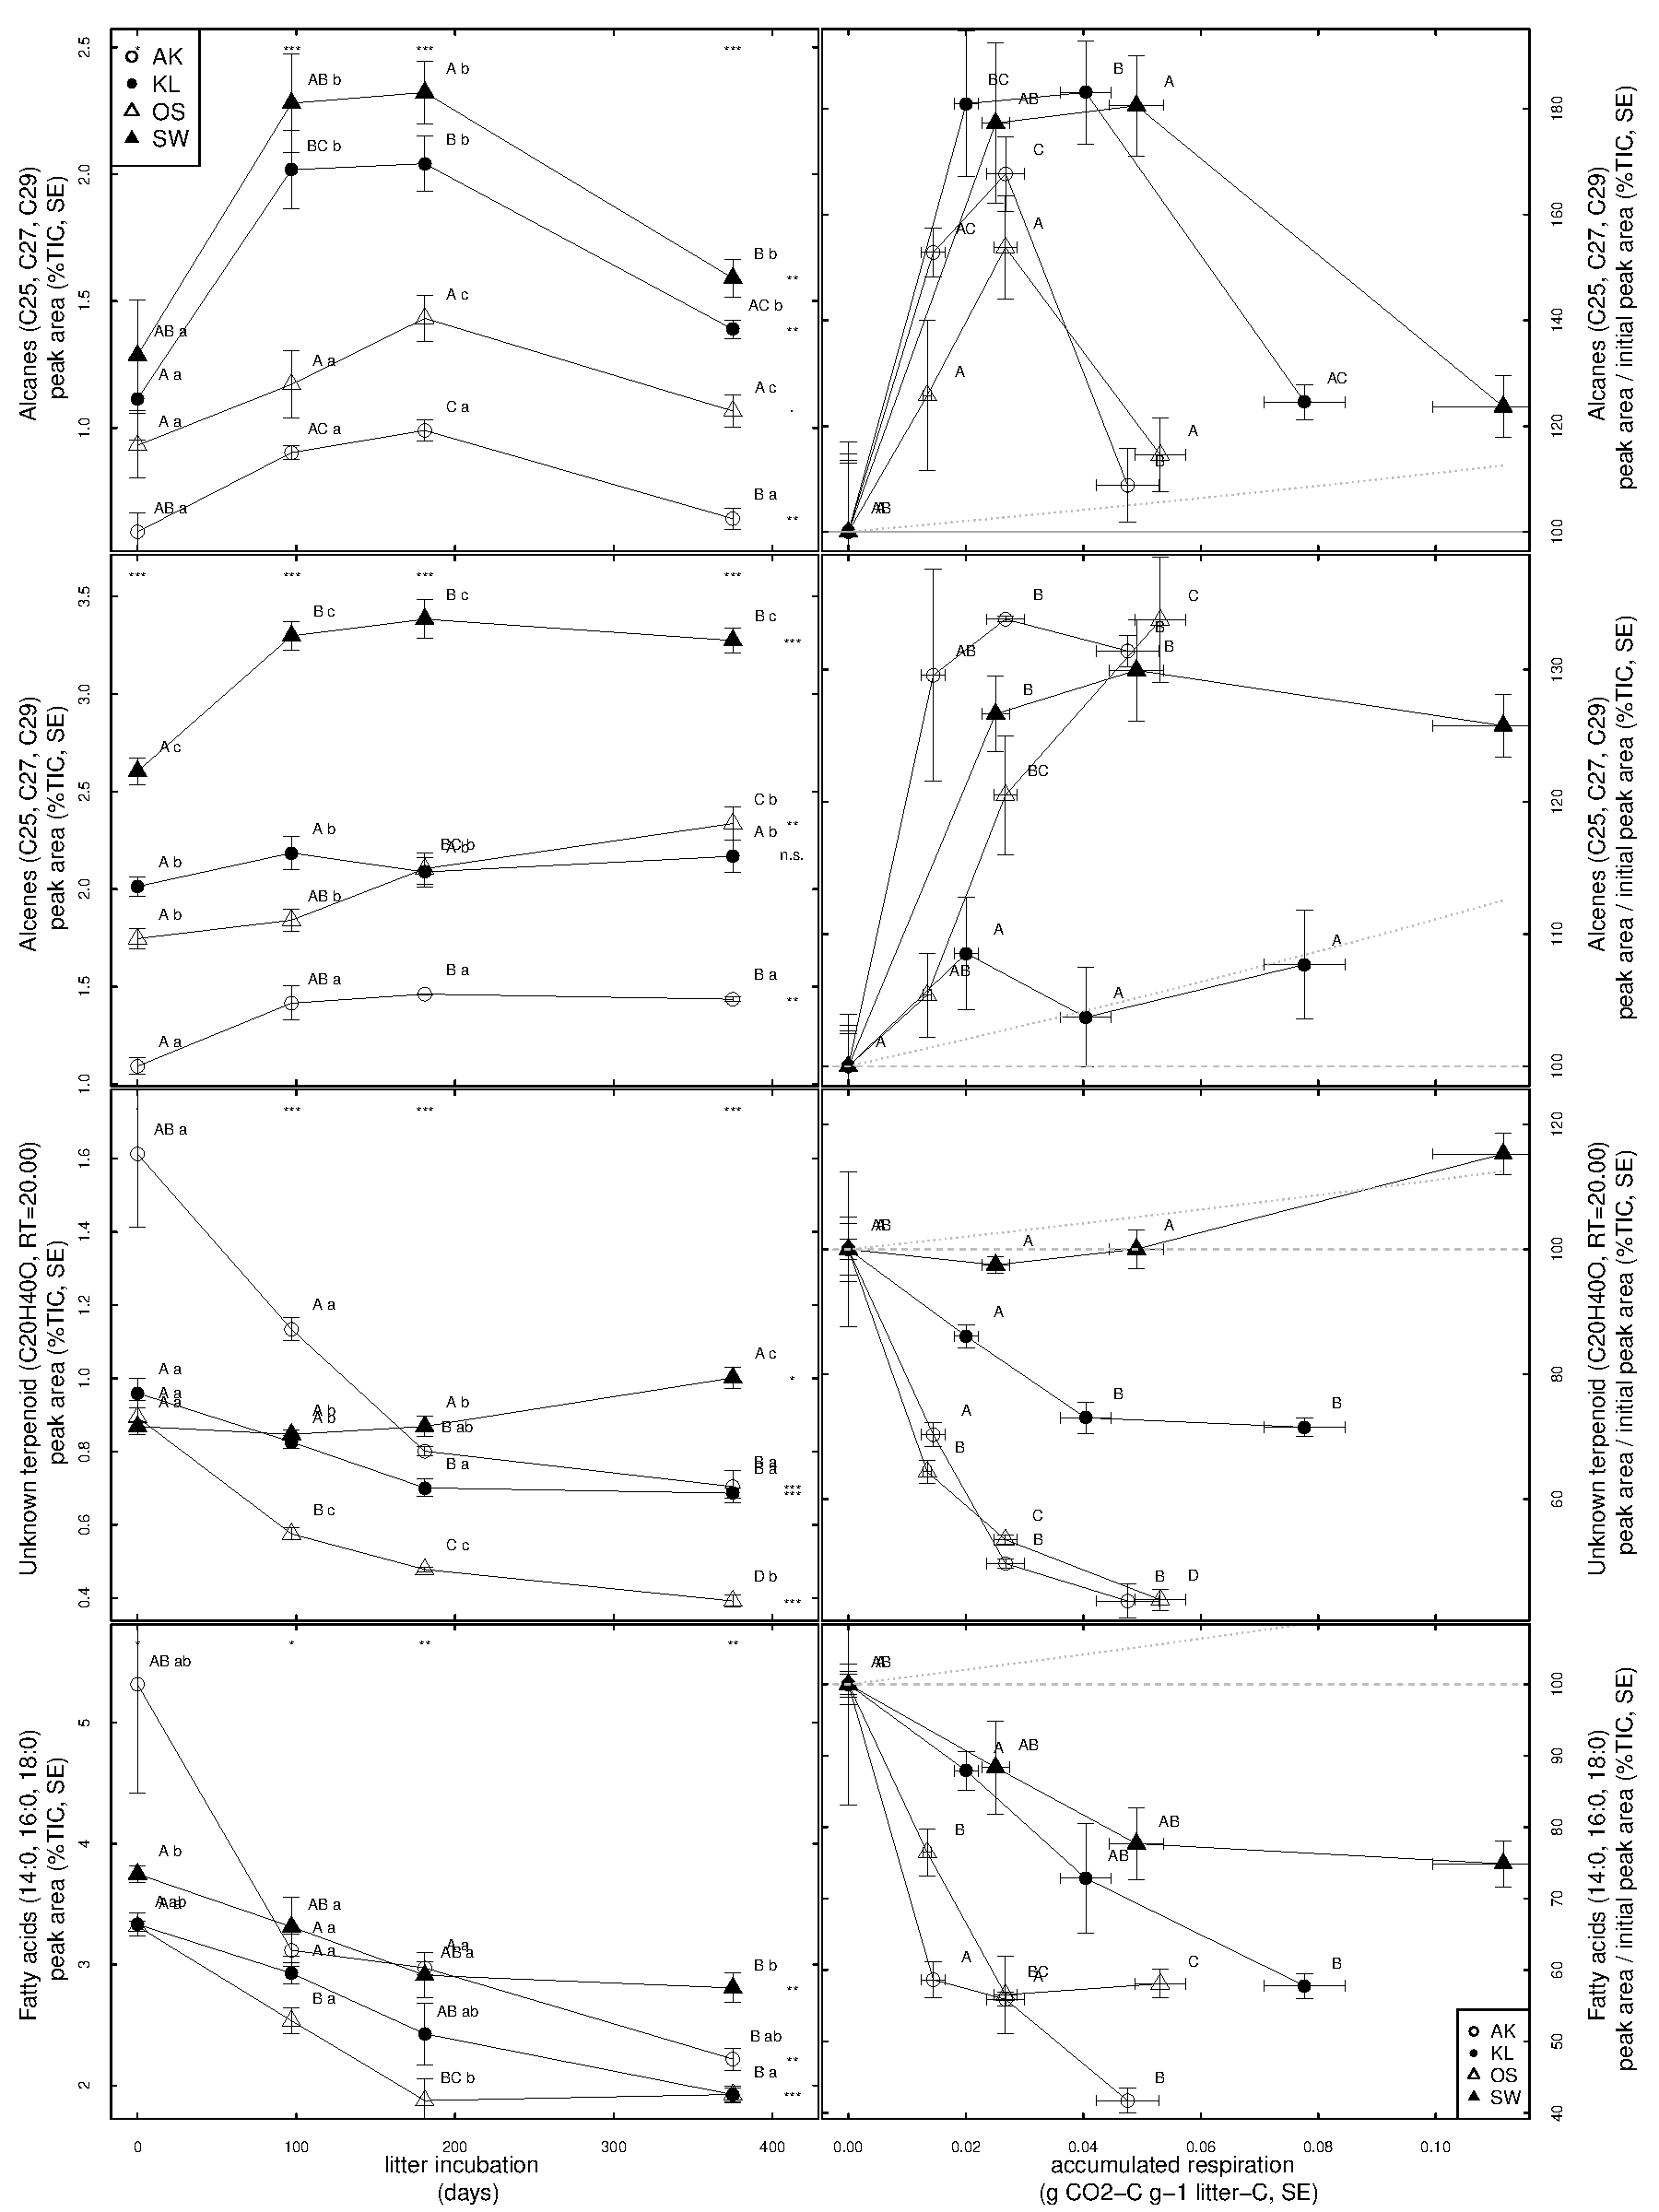
\includegraphics[width=15cm]{timeseries_waxes.pdf}
% %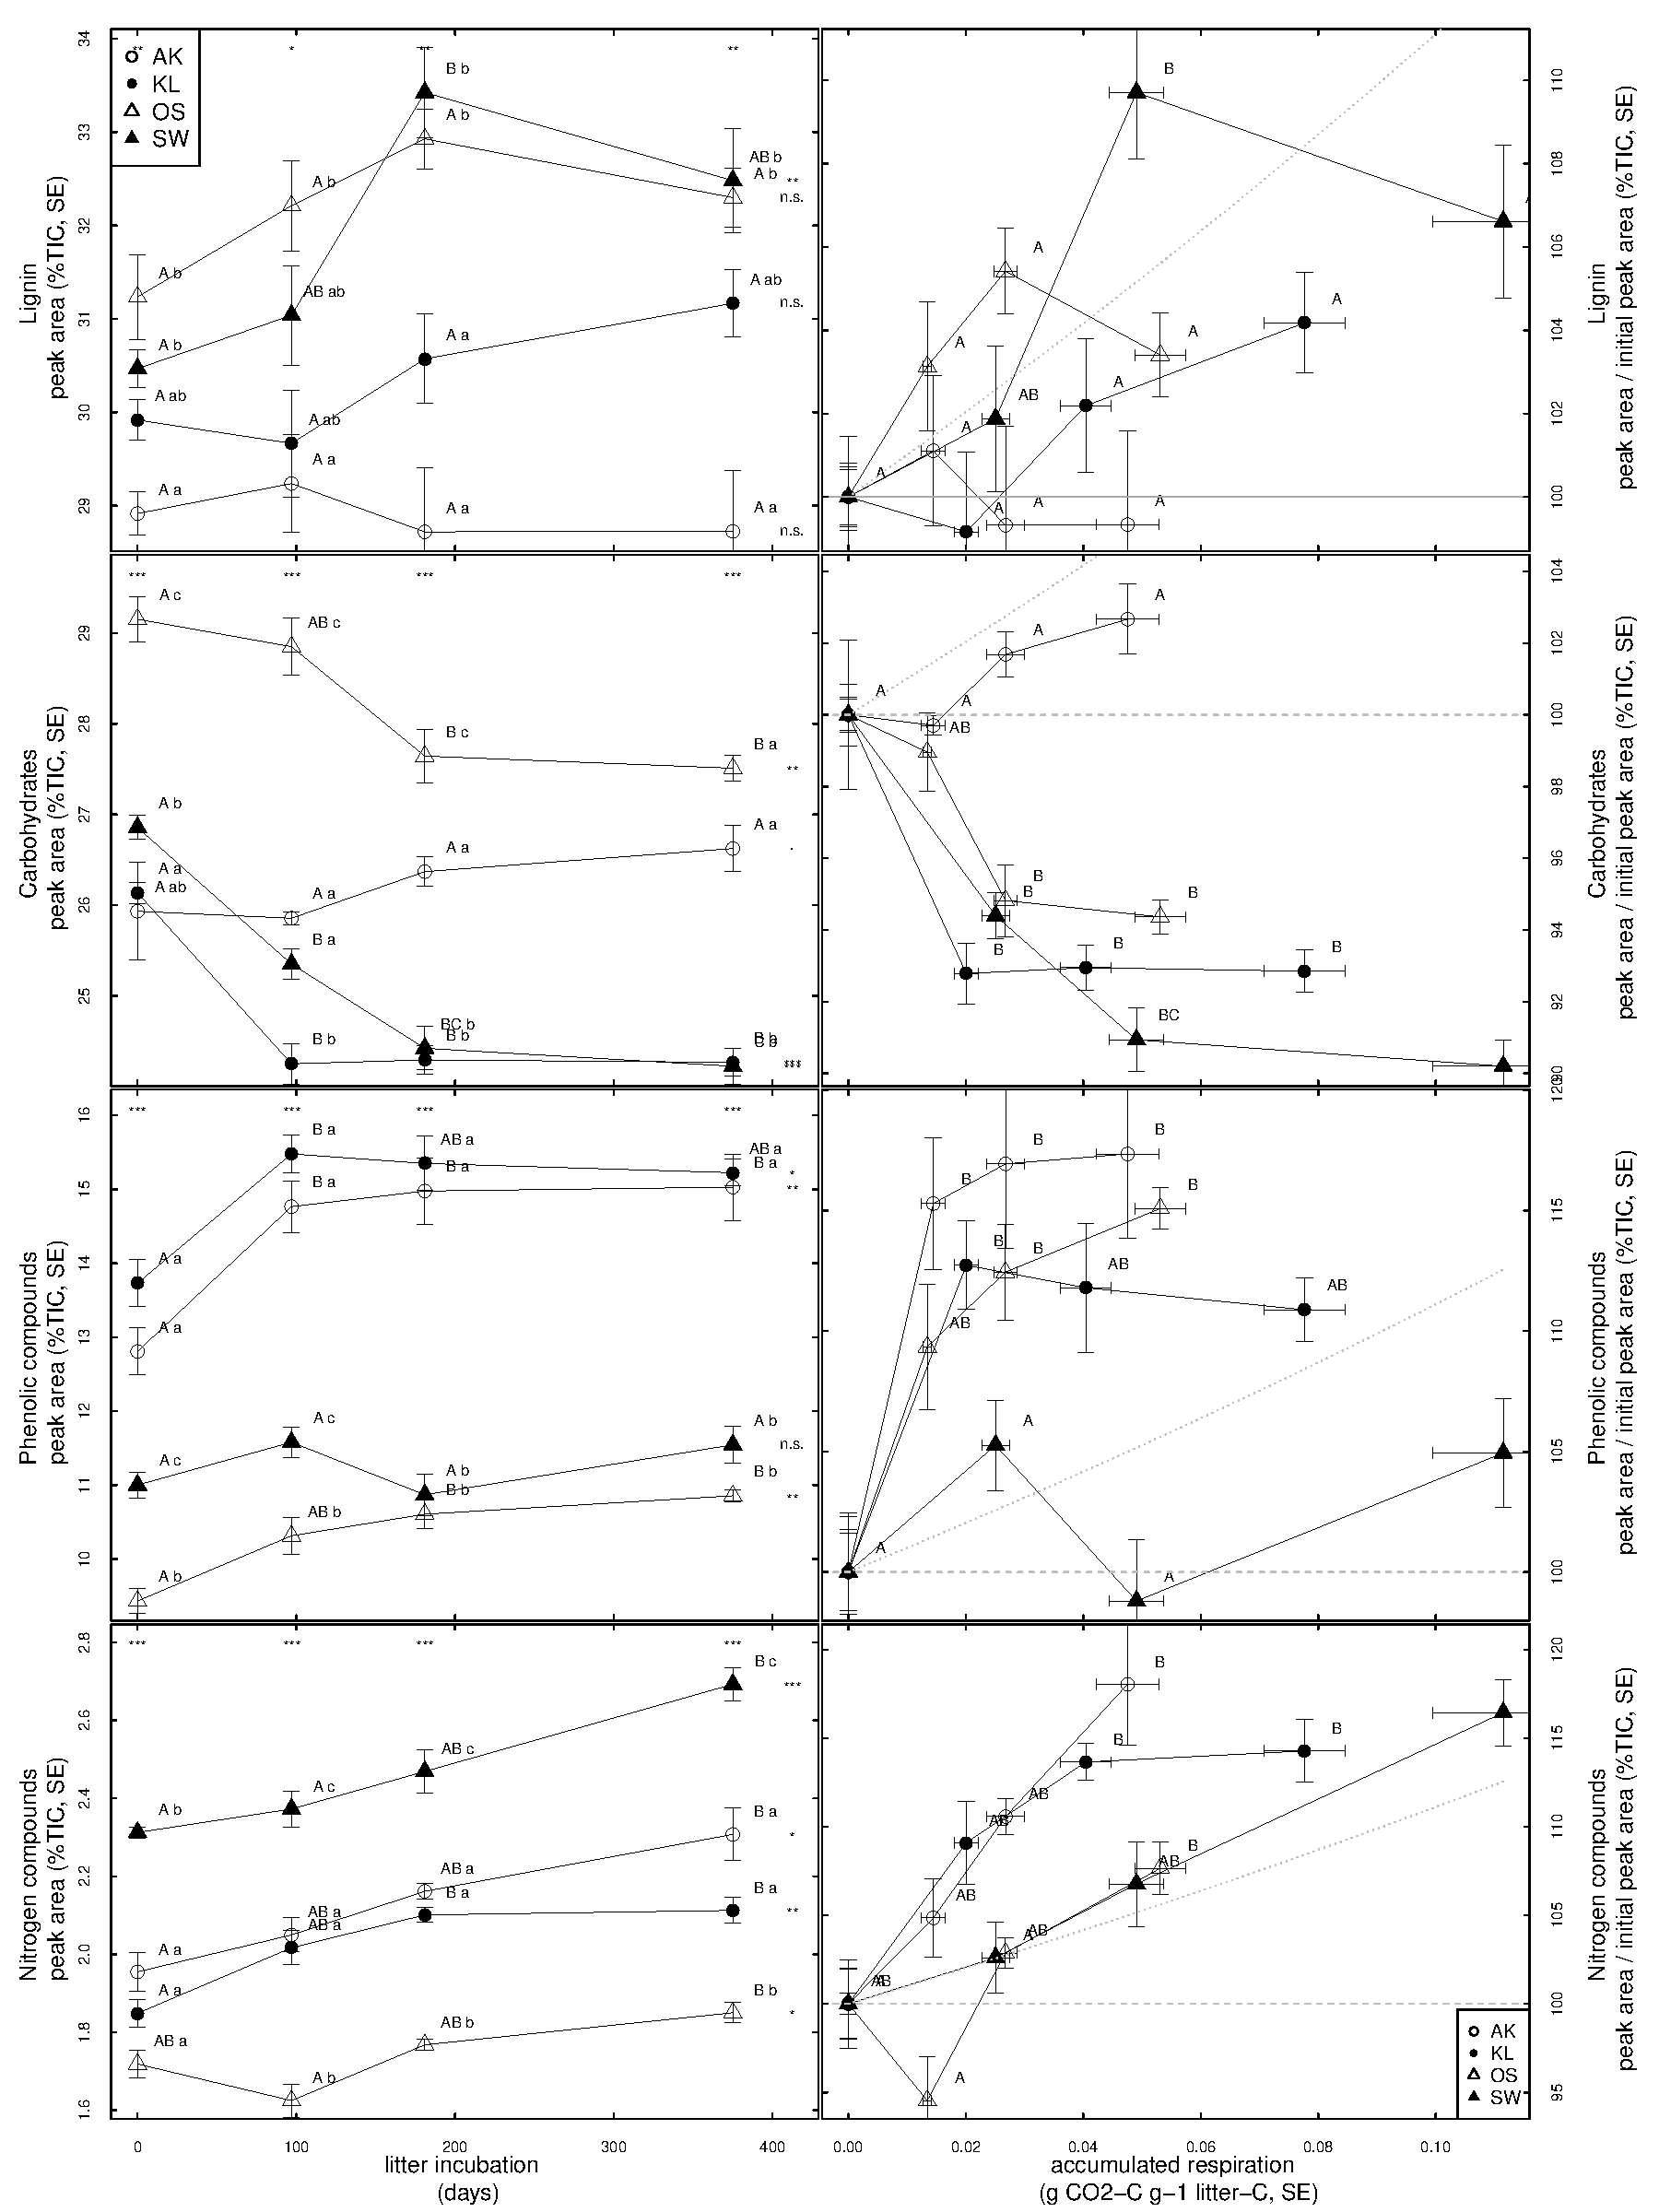
\includegraphics[width=17cm]{timeseries_orig.pdf}
% \end{center}
\caption{Decomposition dynamics of lipophilic compound classes}
\label{fig:waxes}
\end{figure*}





% \begin{figure*}[p]
% \vspace*{2mm}
% \begin{center}
% 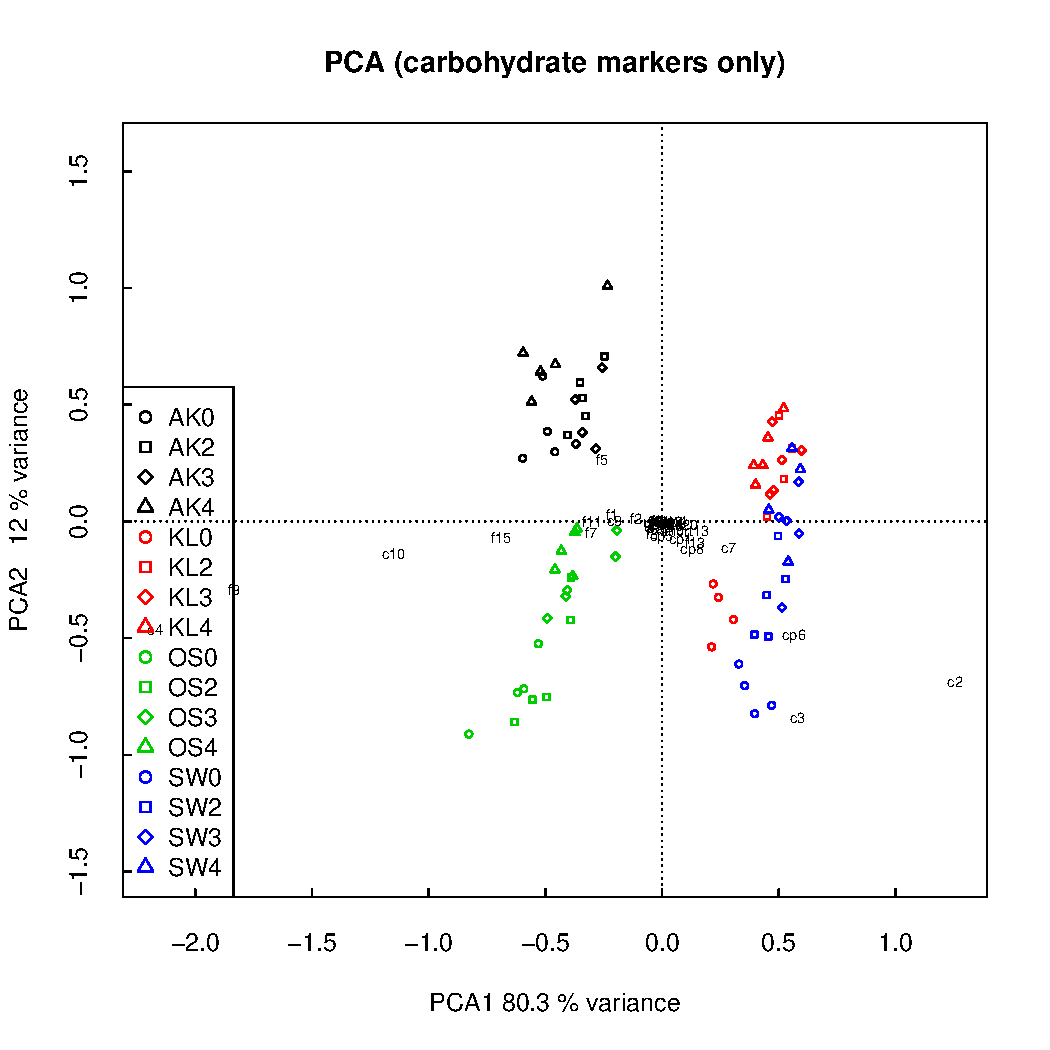
\includegraphics[width=10cm]{pca12_carbos.pdf}
% 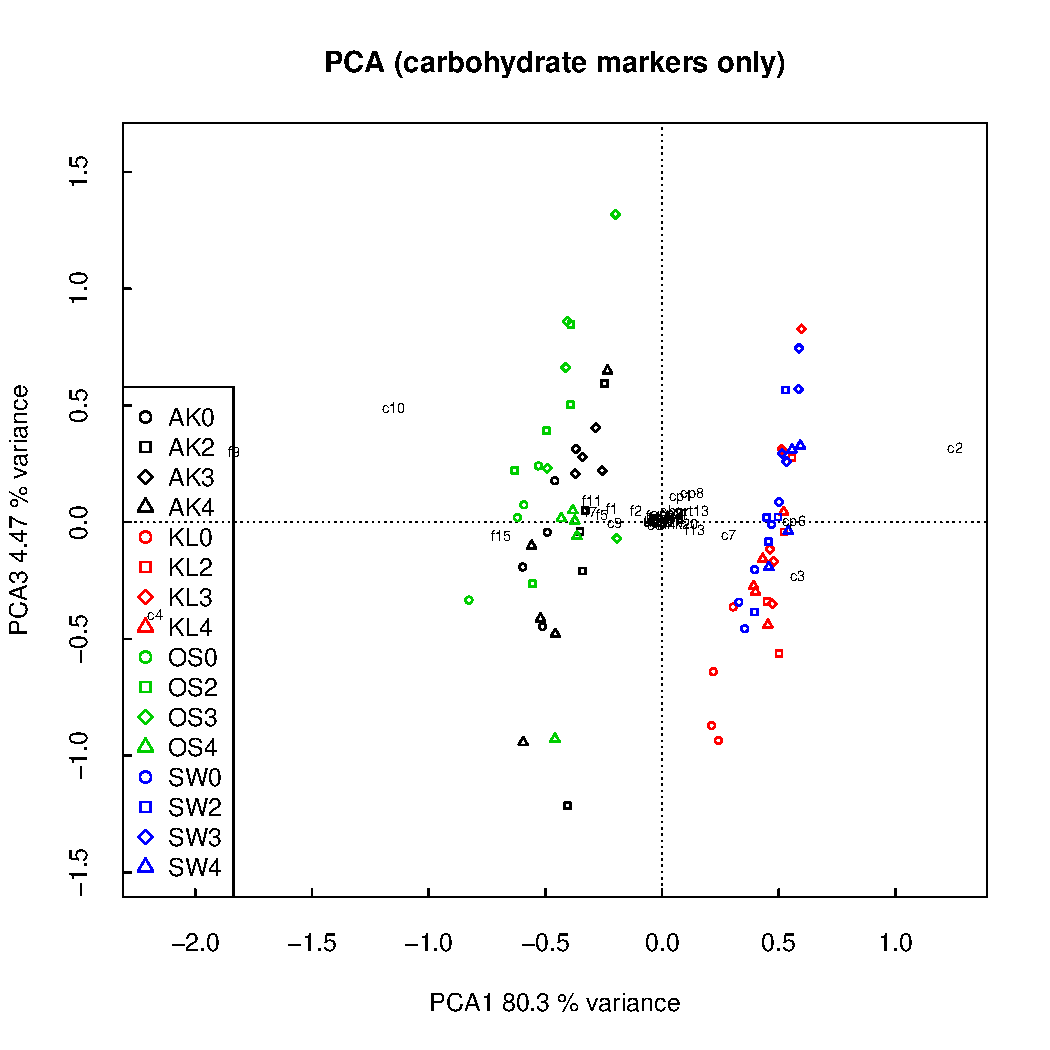
\includegraphics[width=10cm]{pca13_carbos.pdf}
% 
% \end{center}
% \caption{TEXT}
% \end{figure*}
% 
% %% TWO-COLUMN FIGURES
% 
% %f
% \begin{figure*}[p]
% \vspace*{2mm}
% \begin{center}
% \includegraphics[width=10cm]{ligonly_allharvests_PCA12.pdf}
% 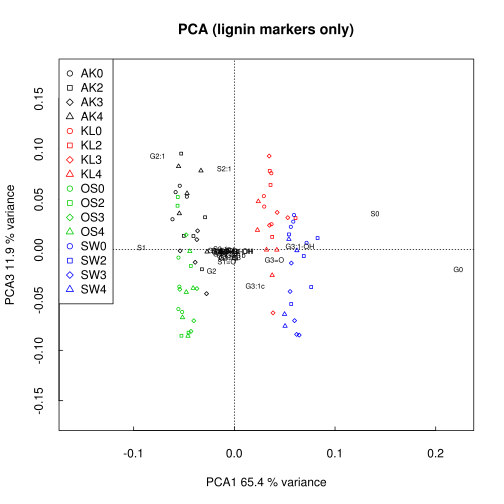
\includegraphics[width=10cm]{ligonly_allharvests_PCA13.pdf}
% \end{center}
% \caption{TEXT}
% \end{figure*}
% 

\newpage
 \begin{figure*}[p]
%  \vspace*{2mm}
%  \begin{center}
%  \includegraphics[width=15cm]{controls_h1.pdf}
%  \end{center}
 \caption{Litter chemistry: content of macro and micronutrients, 14 days after innoculation, n=5}
 \label{fig:litchem_h1}
 \end{figure*}

% \begin{figure*}[p]
% \vspace*{2mm}
% \begin{center}
% \includegraphics[width=12cm]{controls_h2.pdf}
% \end{center}
% \caption{Litter chemistry: content of macro and micronutrients, 97 days after innoculation, n=5}
% \label{fig:litchem_h2}
% \end{figure*}

\newpage
\begin{figure*}[p]
%\vspace*{2mm}
% \begin{center}
% 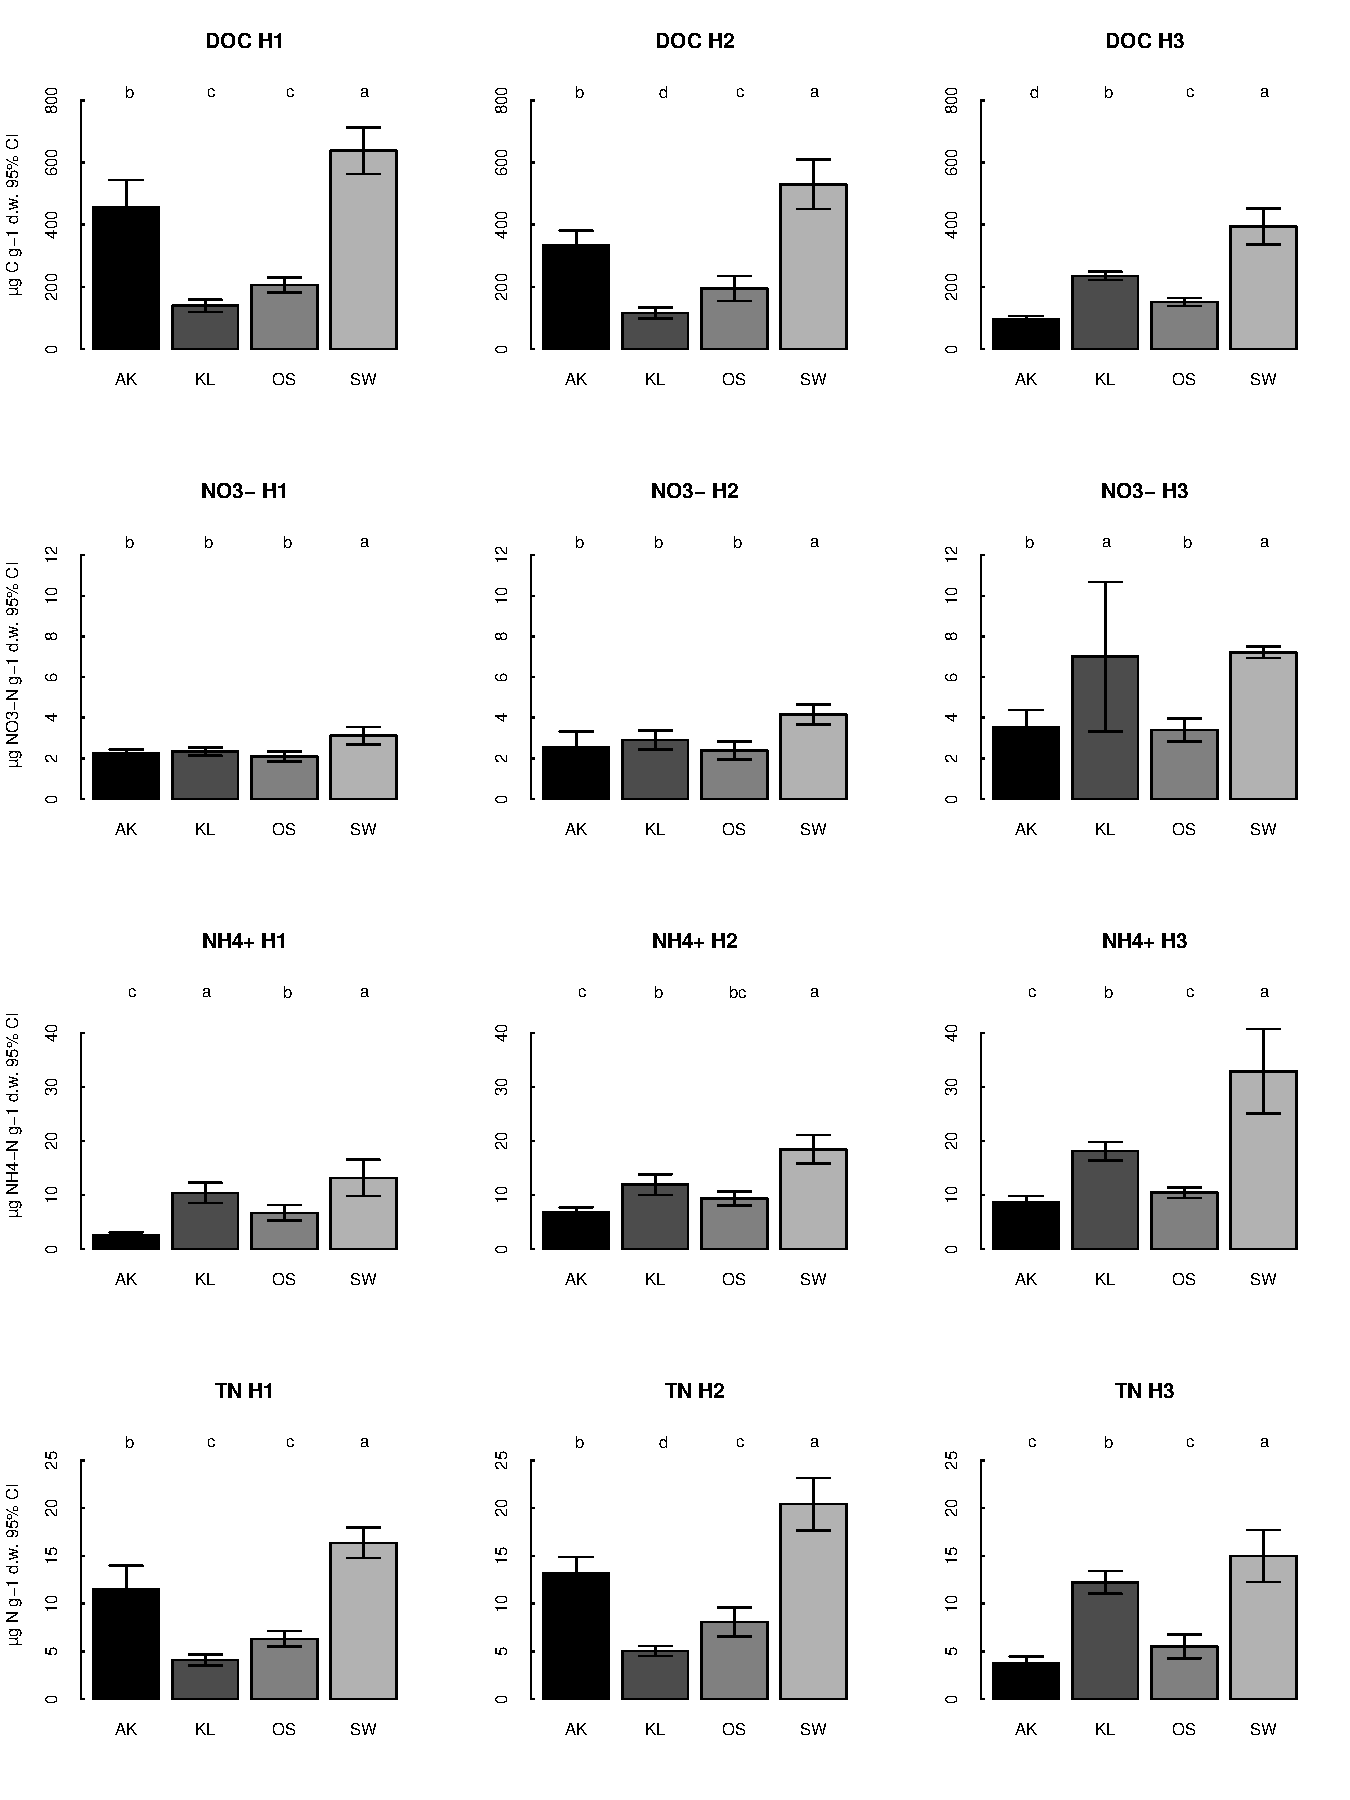
\includegraphics[width=15cm]{doc_barplots.pdf}
% \end{center}
\caption{Litter Chemistry: Dissolved organic carbon, total dissolved nitrogen, NO3-, NH4+}
\label{fig:doc}
\end{figure*}

% \newpage
% \begin{figure*}[p]
% \vspace*{2mm}
% \begin{center}
% 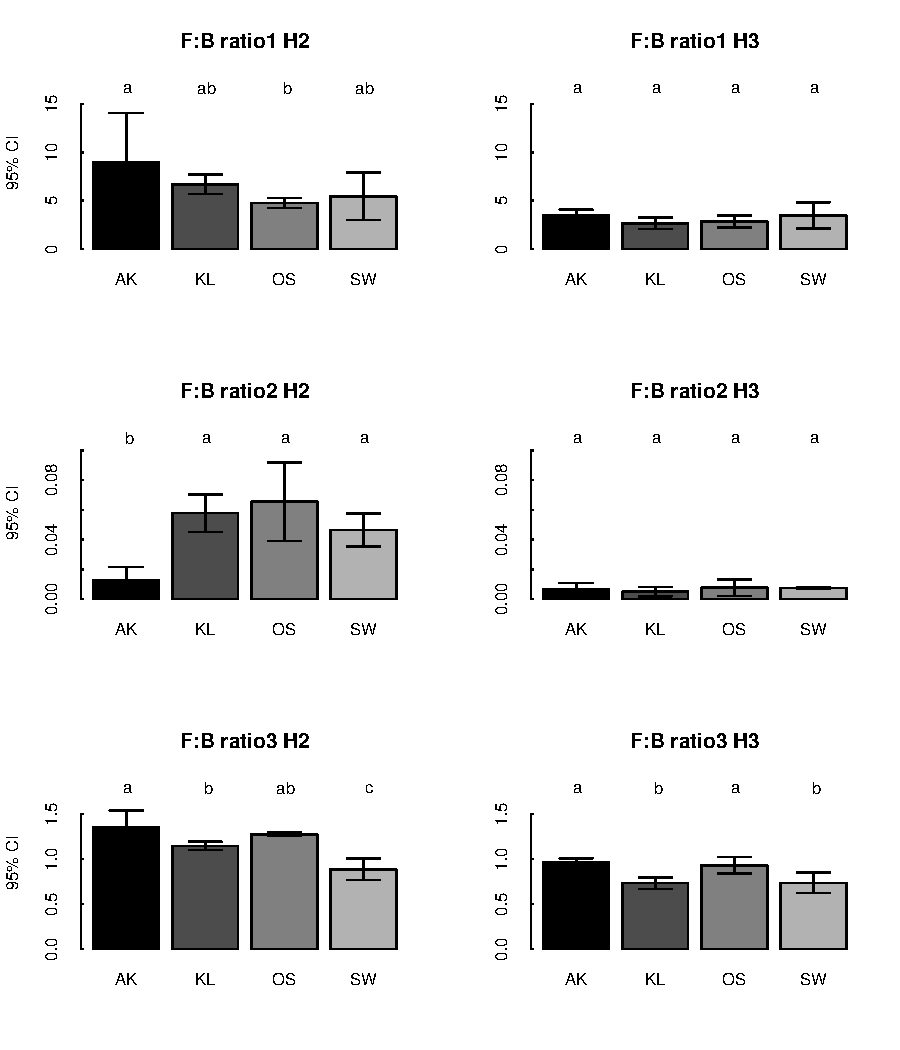
\includegraphics[width=12cm]{plfa.pdf}
% \end{center}
% \caption{Fungi : Bacteria ratios}
% \label{fig:plfa}
% \end{figure*}



\newpage
\begin{table*}[p] 
\begin{tabular}{ccccccc}
Litter type & LCI increase & initial DOC & N & P & Mn & Fe \\
\hline
AK&-&++&-\-&-&-\-&- -\\
KL&++&-\-&-&-\-&+&- -\\
OS&++&-\-&- -&+&-&++\\
SW&++&++&++&++&++&-\-\\
\hline
\end{tabular}
\caption{Summary of context data}
\label{tab:summary}
\end{table*}

%

\newpage
\begin{table*}[p]
\begin{center}
\begin{tabular}{lcccccc}
name & RT & MW & m/z & class\footnotemark[1] & origin\footnotemark[2]&Rf\footnotemark[3]\\
\hline
Furan&2.35&68&39+68&f&C&1.19\\
Methylfuran&2.74&82&81+82&f&C&1.00\\
Methylfuran&2.91&82&81+82&f&C&b.d.l.\\
Dimethylfuran&3.43&96&95+96&f&C&b.d.l.\\
Dimethylfuran&3.66&96&95+96&f&C&1.10\\
Vinylfuran&5.01&94&65+94&f&C&2.59\\
3-Furaldehyd&11.57&96&95+96&f&C&1.65\\
2(5H)Furanon&11.69&98&55+98&f&C&2.41\\
2-Furaldehyd&12.22&96&95+96&f&C&1.67\\
Acetylfuran&12.99&110&95+110&cp&C&2.38\\
5-Methyl-2-furancarboxaldehyde&14.23&110&109+110&f&C&2.44\\
Butyrolactone&15.22&86&56+86&cp&C&12.37\\
Furanmethanol&15.61&98&98&cp&C&5.21\\
5-Methyl-2(5H)-furanone&16.06&98&55+98&f&C&3.92\\
5-hydroxymethylfuran-1-carboxaldehyde&27.51&126&97+126&f&C&2.17\\
2-Oxopropanoic acid, methylester&7.92&102&43+102&cp&C&0.58\\
1-Hydroxypropanone&9.24&74&43&cp&C&1.43\\
Propanoic acid, methylester&12.10&102&43+102&cp&C&1.44\\
2-Cyclopenten-1-one&10.26&82&53+54+52&cp&C&2.02\\
2-Methyl-2-cyclopenten-1-one&10.51&96&53+96&cp&C&2.37\\
3-Methyl-cyclopentanone&13.31&67+96&67+96&cp&C&4.06\\
Dimethylcyclopentenone&13.69&110&67+95+110&cp&C&1.63\\
2-Cyclopenten-1,4-dione&14.44&96&54+68+96&cp&C&1.68\\
1,2-Cylopentandione&17.51&98&55+98&cp&C&2.22\\
2-Hydroxy-3-methyl2-cyclopenten-1-one&18.14&98&98&cp&C&15.96\\
3-Methyl-1,2-cyclopentanedione&18.42&112&69+112&cp&C&2.73\\
Laevoglucosan&40.44&60+73&60+73&f&C&0.00\\
unknown carbohydrate&19.06&58+86+114&58+86+114&f&C&1.83\\
unknown carbohydrate&19.35&98+126&98+126&cp&C&5.35\\
unknown carbohydrate&21.77&116&116&f&C&b.d.l.\\
unknown carbohydrate&22.33&44&44&cp&C&3.34\\
unknown carbohydrate&26.18&57+69&57+69&f&C&1.15\\
unknown carbohydrate&31.67&73+135&73+135&f&C&7.59\\
Toluene&&&&ar&non&b.d.l.\\
Xylene&&&&ar&non&4.46\\
Xylene&&&&ar&non&b.d.l.\\
Xylene&&&&ar&non&b.d.l.\\
Methoxymethylbenzene&&&&ar&non&4.04\\
benzaldehyde&&&&ar&non&12.88\\
Phenol&21.02&&&ph&Ph&1.72\\
4-Methylphenol&22.11&&&ph&Ph&1.70\\
3-Methylphenol&22.22&&&ph&Ph&1.35\\
4-Ethylphenol&23.38&&&ph&Ph&1.36\\
4-Propenylphenol[1]&26.93&&&ph&Ph&5.13\\
4-Propenylphenol[2]&27.76&134&133+134&ph&Ph&4.78\\
4-Propylphenol&31.11&&&ph&Ph&1.39\\
Butylphenol&31.86&&&ph&Ph&2.42\\%peak assignment unsure
Hydroquinon&33.4&&&ph&Ph&2.14\\%w/ Resorcinol
\hline
\end{tabular}
 \footnotetext[1]{cp: Cyclopentenone - type f: Furane-type}
 \footnotetext[2]{C: Carbohydrate pyrolysis products}
 \footnotetext[3]{Rf: see section .. b.d.l.: peak is below detection limit in TIC integration.}
 \caption{Table with rows, columns and footnotes}
\end{center}
\label{tab:pyrprod1}
\end{table*}


\begin{table*}
\begin{center}
\begin{tabular}{lcccccc}
name & RT & MW & m/z & class & origin&Rf\\
\hline
Guaiacol&18.87&124&109+124&g&L&2.48\\
Methylguaiacol&20.32&138&123+138&g&L&1.93\\
Ethylguaiacol&21.4&152&137+152&g&L&2.18\\
Propenylguaiacol [1]&23.29&164&149+164&g&L&3.30\\
Ethylenguaiacol&23.69&150&135+150&g&L&2.05\\
Propenylguaiacol [2]&24.48&164&149+164&g&L&14.20\\
Syringol&24.58&154&139+154&sy&L&2.37\\
Propenylguaiacol [3]&25.66&164&149+164&g&L&5.01\\
Methylsyringol&25.67&168&153+168&sy&L&0.00\\
Ethylsyringol&26.39&182&167+182&sy&L&1.70\\
Propenylsyringol [1]&27.97&194&179+194&sy&L&4.58\\
Ethylensyringol&28.37&180&165+180&sy&L&5.10\\
Gaiacolaldehyde&28.4&152&109+152&g&L&0.00\\
Propanylguaiacol&28.72&166&137+166&g&L&1.47\\
Oxo-hydroxy-propanylguaiacol&28.77&182&182&g&L&20.45\\
Propenylsyringol [2]&28.91&194&179+194&sy&L&2.71\\
G2=O&29.2&166&151+166&g&L&1.69\\
G3=O&29.36&180&137+180&g&L&1.70\\
S3:1c&30.16&194&194+179&sy&L&3.76\\
S1=O&32.68&182&139+182&sy&L&7.20\\
Ph1=O&32.7&122&121+122&ph&Ph&0.00\\
S3=O/-OH&32.8&212&212&sy&L&0.00\\
GAc&32.88&182&137+182&g&L&2.04\\
S3&33.15&196&181+196&sy&L&3.05\\
S3=O&33.32&210&167+210&sy&L&1.64\\
G3:1=O&35.3&178&135+178&g&L&4.12\\
G3:1-OH&37.1&137+180&180&g&L&2.08\\
SAc&38.78&212&212&sy&L&4.78\\
S3:1=O&43.06&208&165+208&sy&L&2.96\\

N-methyl-pyrrol&&&&p&N&5.47\\
pyridine&&&&p&N&1.68\\
methylpyridine1&&&&p&N&1.41\\
methylpyridine2&&&&p&N&0.55\\
pyrrole&&&&p&N&1.89\\
methylpyrrol1&&&&p&N&1.84\\
methylpyrrol2&&&&p&N&2.30\\
Pyridol&&&&unk&unk&2.11\\
Indole&&&&ind&N&2.97\\
Methylindole&&&&ind&N&0.00\\
25:0&&&&cut0&Cut&3.16\\
25:1&&&&cut1&Cut&13.32\\
27:0&&&&cut0&Cut&2.97\\
27:1&&&&cut1&Cut&6.24\\
29:0&&&&cut0&Cut&4.47\\
29:1&&&&cut1&Cut&13.82\\
14:0fa&2.35&68&39+68&fa&lip&50\\
16.0fa&2.74&82&81+82&fa&lip&62.67\\
18:0fa&2.91&82&81+82&fa&lip&29.59\\

\hline
\end{tabular}
\end{center}
\label{tab:pyrprod2}
\end{table*}


\begin{table*}
\begin{center}
\begin{tabular}{lcccccc}
name & RT & MW & m/z & class & origin&Rf\\
\hline
alcene 5.61+5.67&&&&al&al&5.83\\
propanol 5.62&&&&short&non&0.00\\
unknown furan 6.36&&&&f&C&1.93\\
cyclopentanone 6.99&&&&cp&C&0.00\\
xylene4 6.99&&&&ar&non&4.07\\
limonen 7.29&&&&ter&non&0.59\\
methylpyridine3 7.54&&&&p&N&1.88\\
methylfurane2 7.64&&&&f&C&2.00\\
unknown 8.14&&&&unk&unk&10.20\\
alcene 9.55&&&&al&al&5.79\\
alcene 9.71+9.77&&&&al&al&9.77\\
alcene 9.87&&&&al&al&7.33\\
1-Hydroxy-2-propanone&10.69&&cp&C&2.46\\
unknown ch 11.38&&&&cp&C&4.66\\
alcane 11.89&&&&al&al&3.17\\
indene 12.64&&&&ar&non&0.79\\
unknown ch 15.56&&&&cp&C&119.68\\
1-Methyl-4-methoxybenzene&15.98&&&ar&non&10.92\\
unknown ch 16.17&&&&cp&C&2.58\\
unknown 17.67&&&&cp&C&1.16\\
4(H)pyran-4-one 18.25&&&&o&non&2.70\\
unknown alcyl 20.00&&&&al&al&9.39\\
unknown 20.85&&&&unk&unk&7.94\\
unknown 20.86&&&&unk&unk&0.00\\
unknown 22.43&&&&unk&unk&3.88\\
unknown alkyl 22.82&&&&al&unk&12.46\\
hexan2,4dione, -enol 23.92&&&&o&unk&1.19\\
benzofuran 26.19&&&&bf&unk&1.45\\
unknown 27.76&&&&unk&unk&163.60\\

Acetaldehyde&2.06&44&29+44&cp&C&1.04\\
Aceton&2.46&&&short&non&1.65\\
2-Propenal&2.6&&&short&non&1.75\\
Methanol&2.88&&&short&non&1.36\\
3-Buten-2-one&3.39&&&short&non&2.93\\
2,3-Butandione&3.67&&&short&non&1.58\\
3-Penten-2-one&3.89&&&short&non&3.55\\
2-Butanal&4.56&&&short&non&0.00\\
2,3-Pentadione&4.77&&&short&non&2.46\\
Hexanal&5.16&&&short&non&2.85\\
1-Penten-3-one&11.28&&&short&non&2.14\\
\hline
\end{tabular}
\end{center}
\label{tab:pyrprod3}
\end{table*}


%% \begin{figure}[p]
% \vspace*{2mm}
% \begin{center}
% 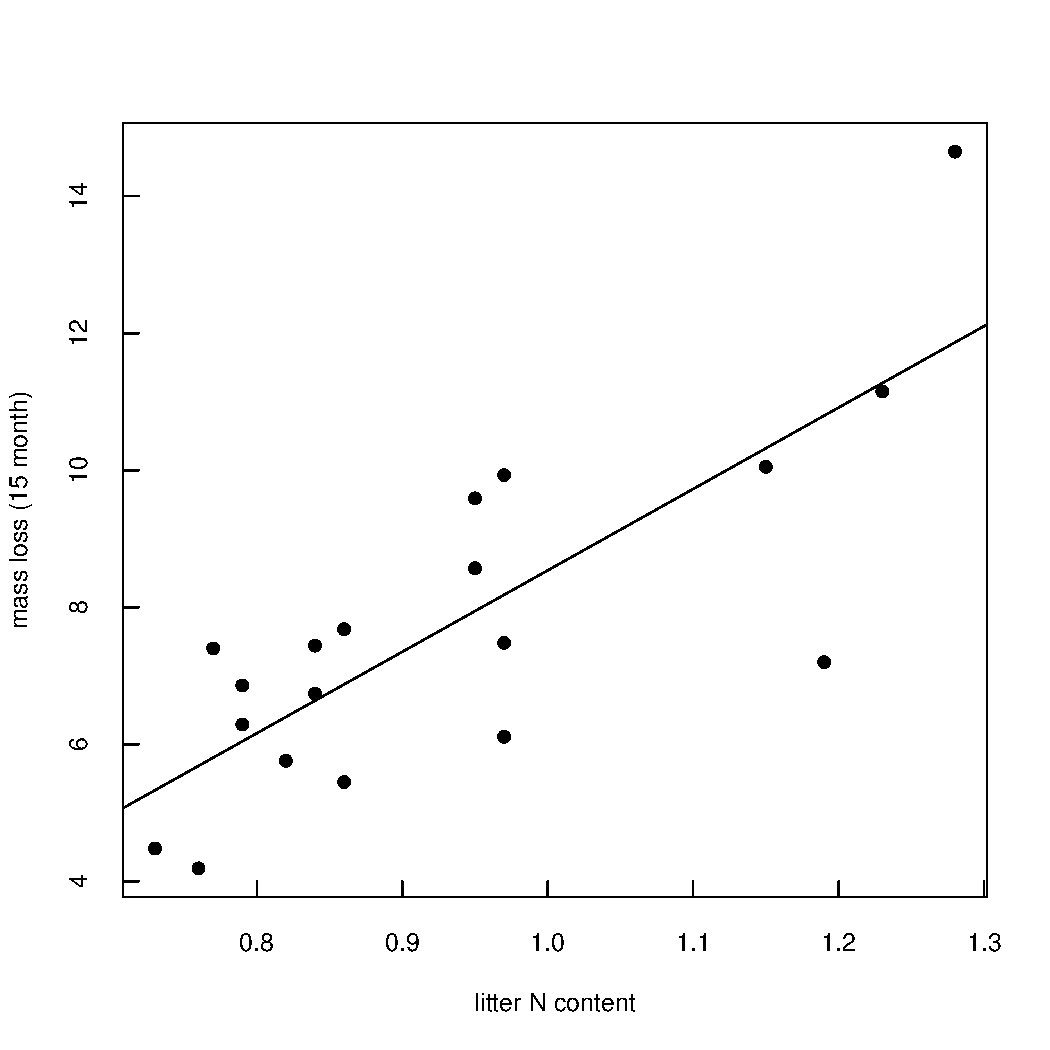
\includegraphics[width=8.3cm]{massloss_n_lit.pdf}
% \end{center}
% \label{fig:n_massloss}
% \caption{Litter mass loss after 15 month vs. litter N content. R= 0.795, p \textless .001}
% \end{figure}

% \newpage
% \begin{figure}[p]
% \vspace*{2mm}
% \begin{center}
% 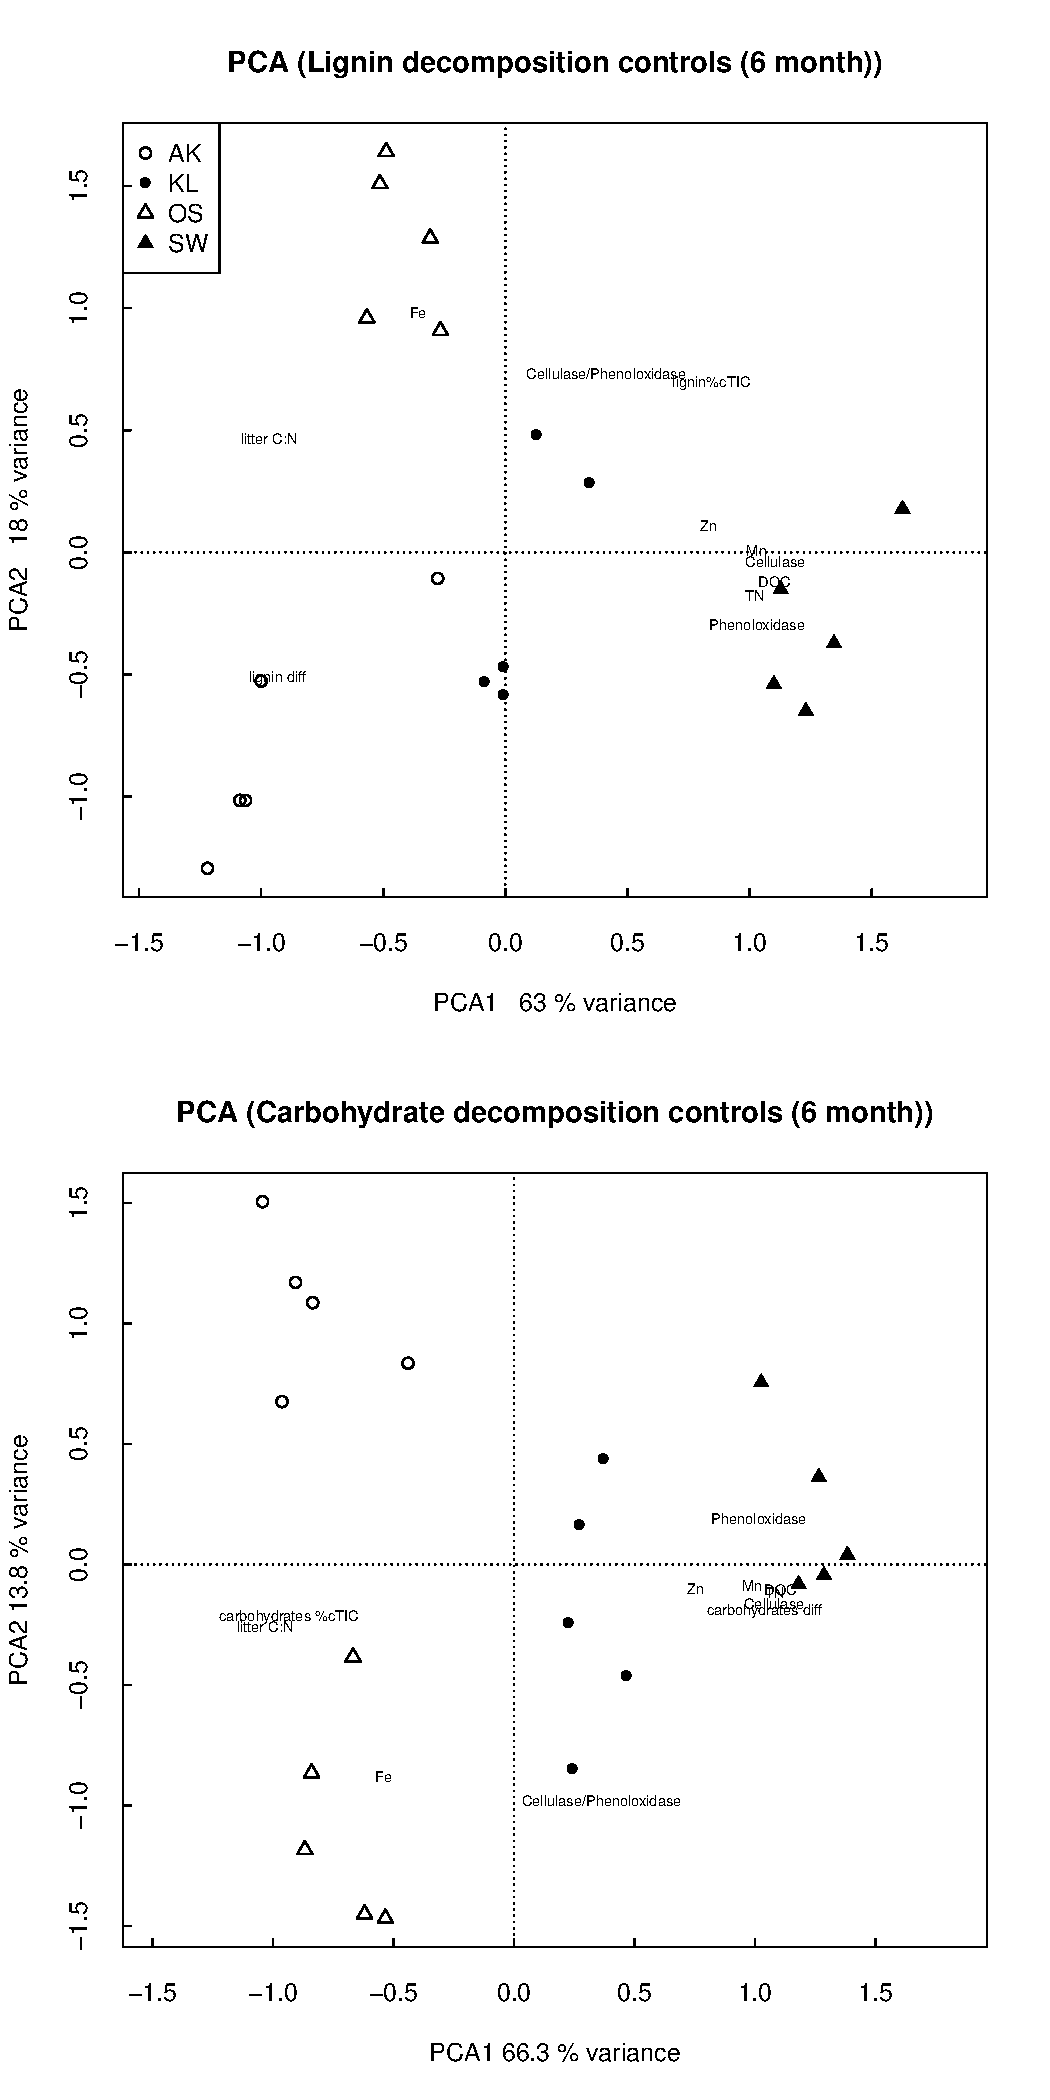
\includegraphics[width=8.3cm]{h3_decomp_contr.pdf}
% \end{center}
% \caption{Litter mass loss after 15 month vs. litter N content. R= 0.795, p \textless .001}
% \label{fig:h3_controls}
% \end{figure}

% \newpage
% \begin{figure*}[p]
% \vspace*{2mm}
% \begin{center}
% 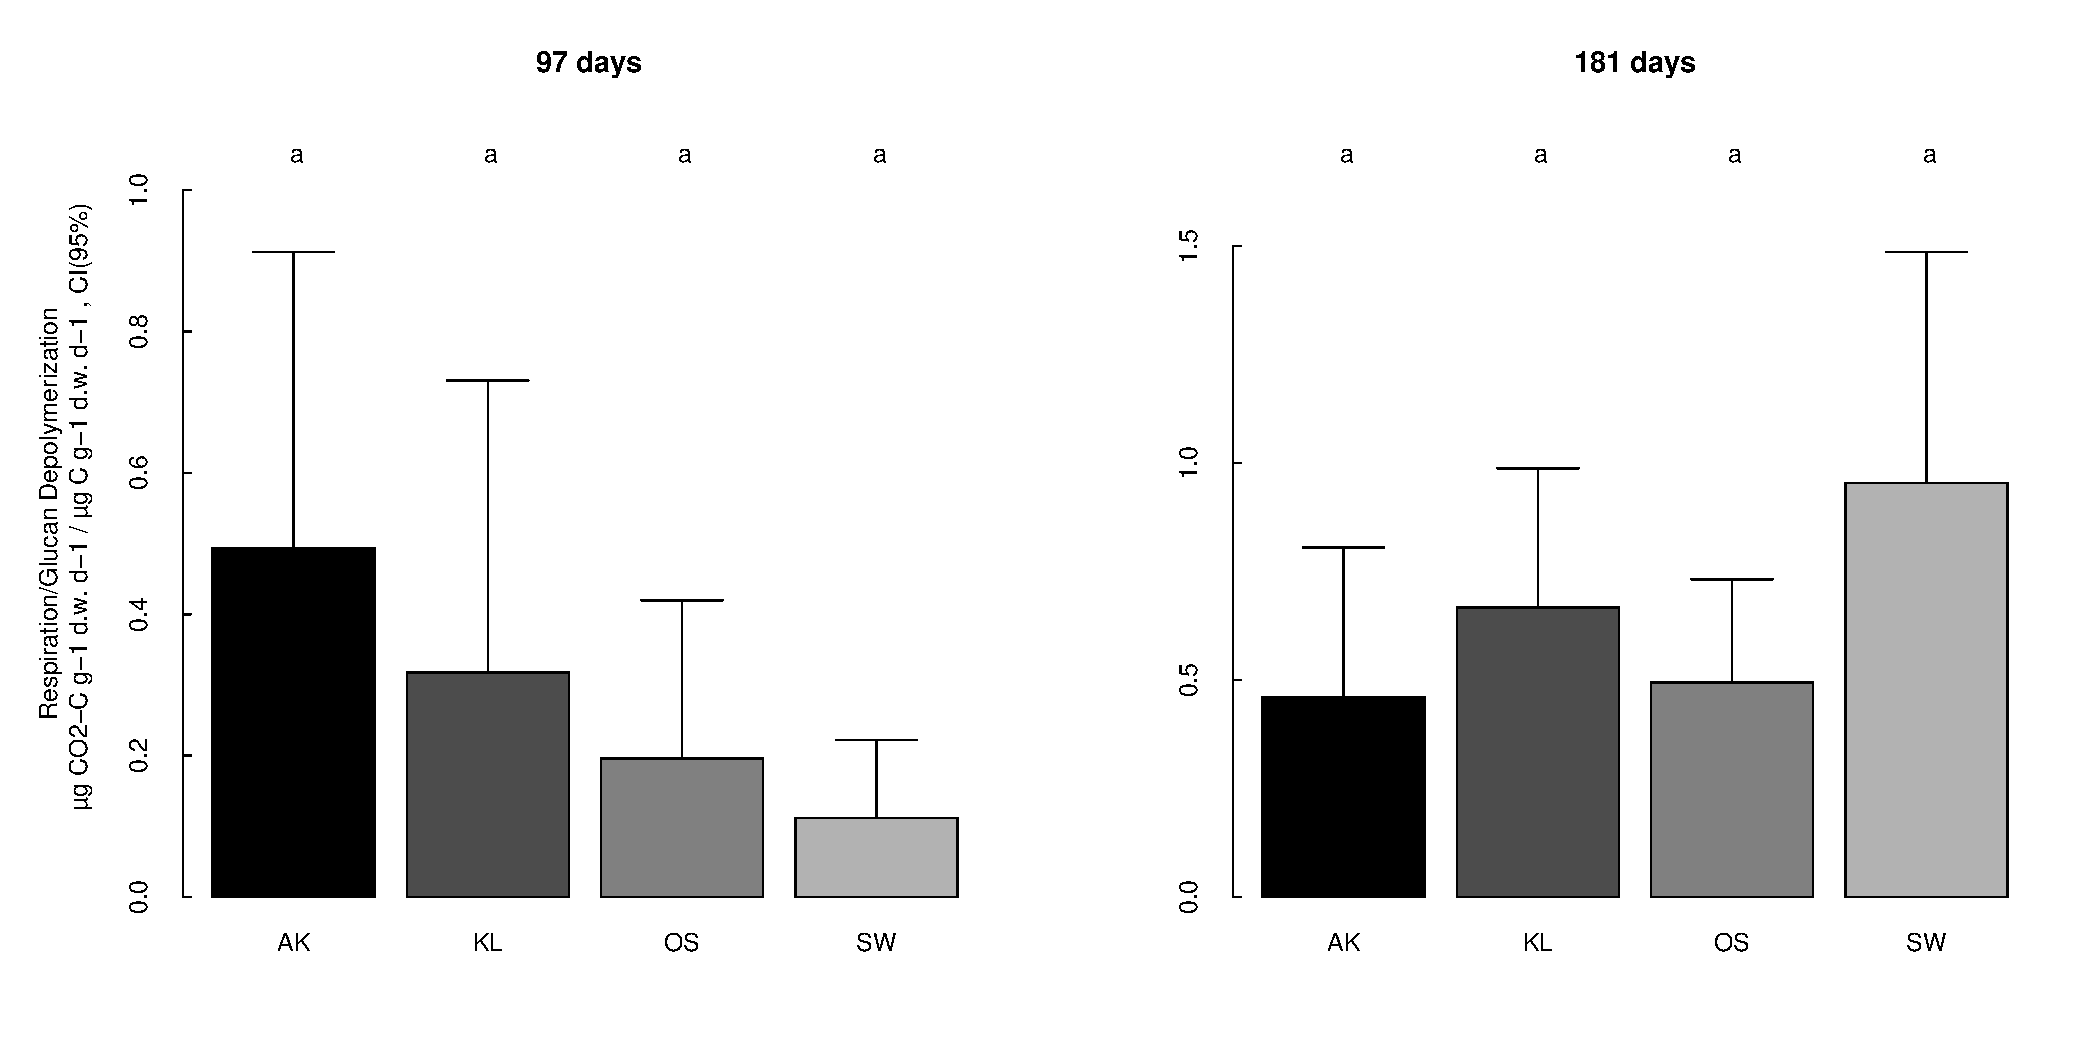
\includegraphics[width=12cm]{resp_glcdepoly_h23.pdf}
% \end{center}
% \caption{Quotient of respiration and glucan depolymerization. In AK microbial community respire significantly more non-glucose carbon after 2, but not after 6 month. Data from \cite{Leitner2011}}
% \label{fig:resp_depoly}
% \end{figure*}

\newpage
\begin{figure*}[p]
\vspace*{2mm}
\begin{center}
%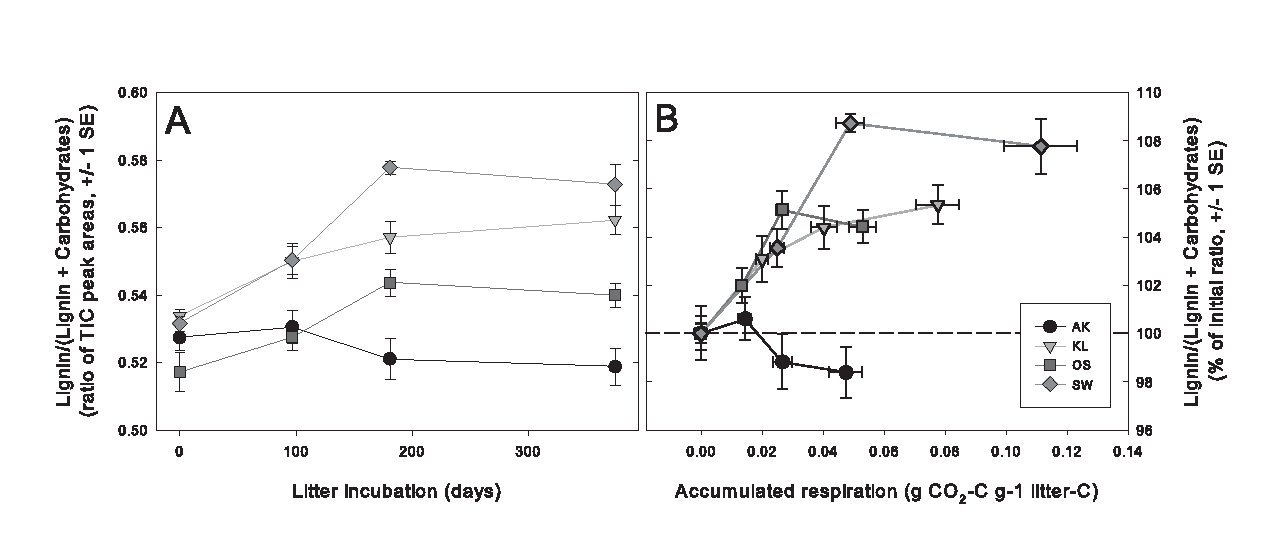
\includegraphics[width=15cm]{graph1_lci.EPS}
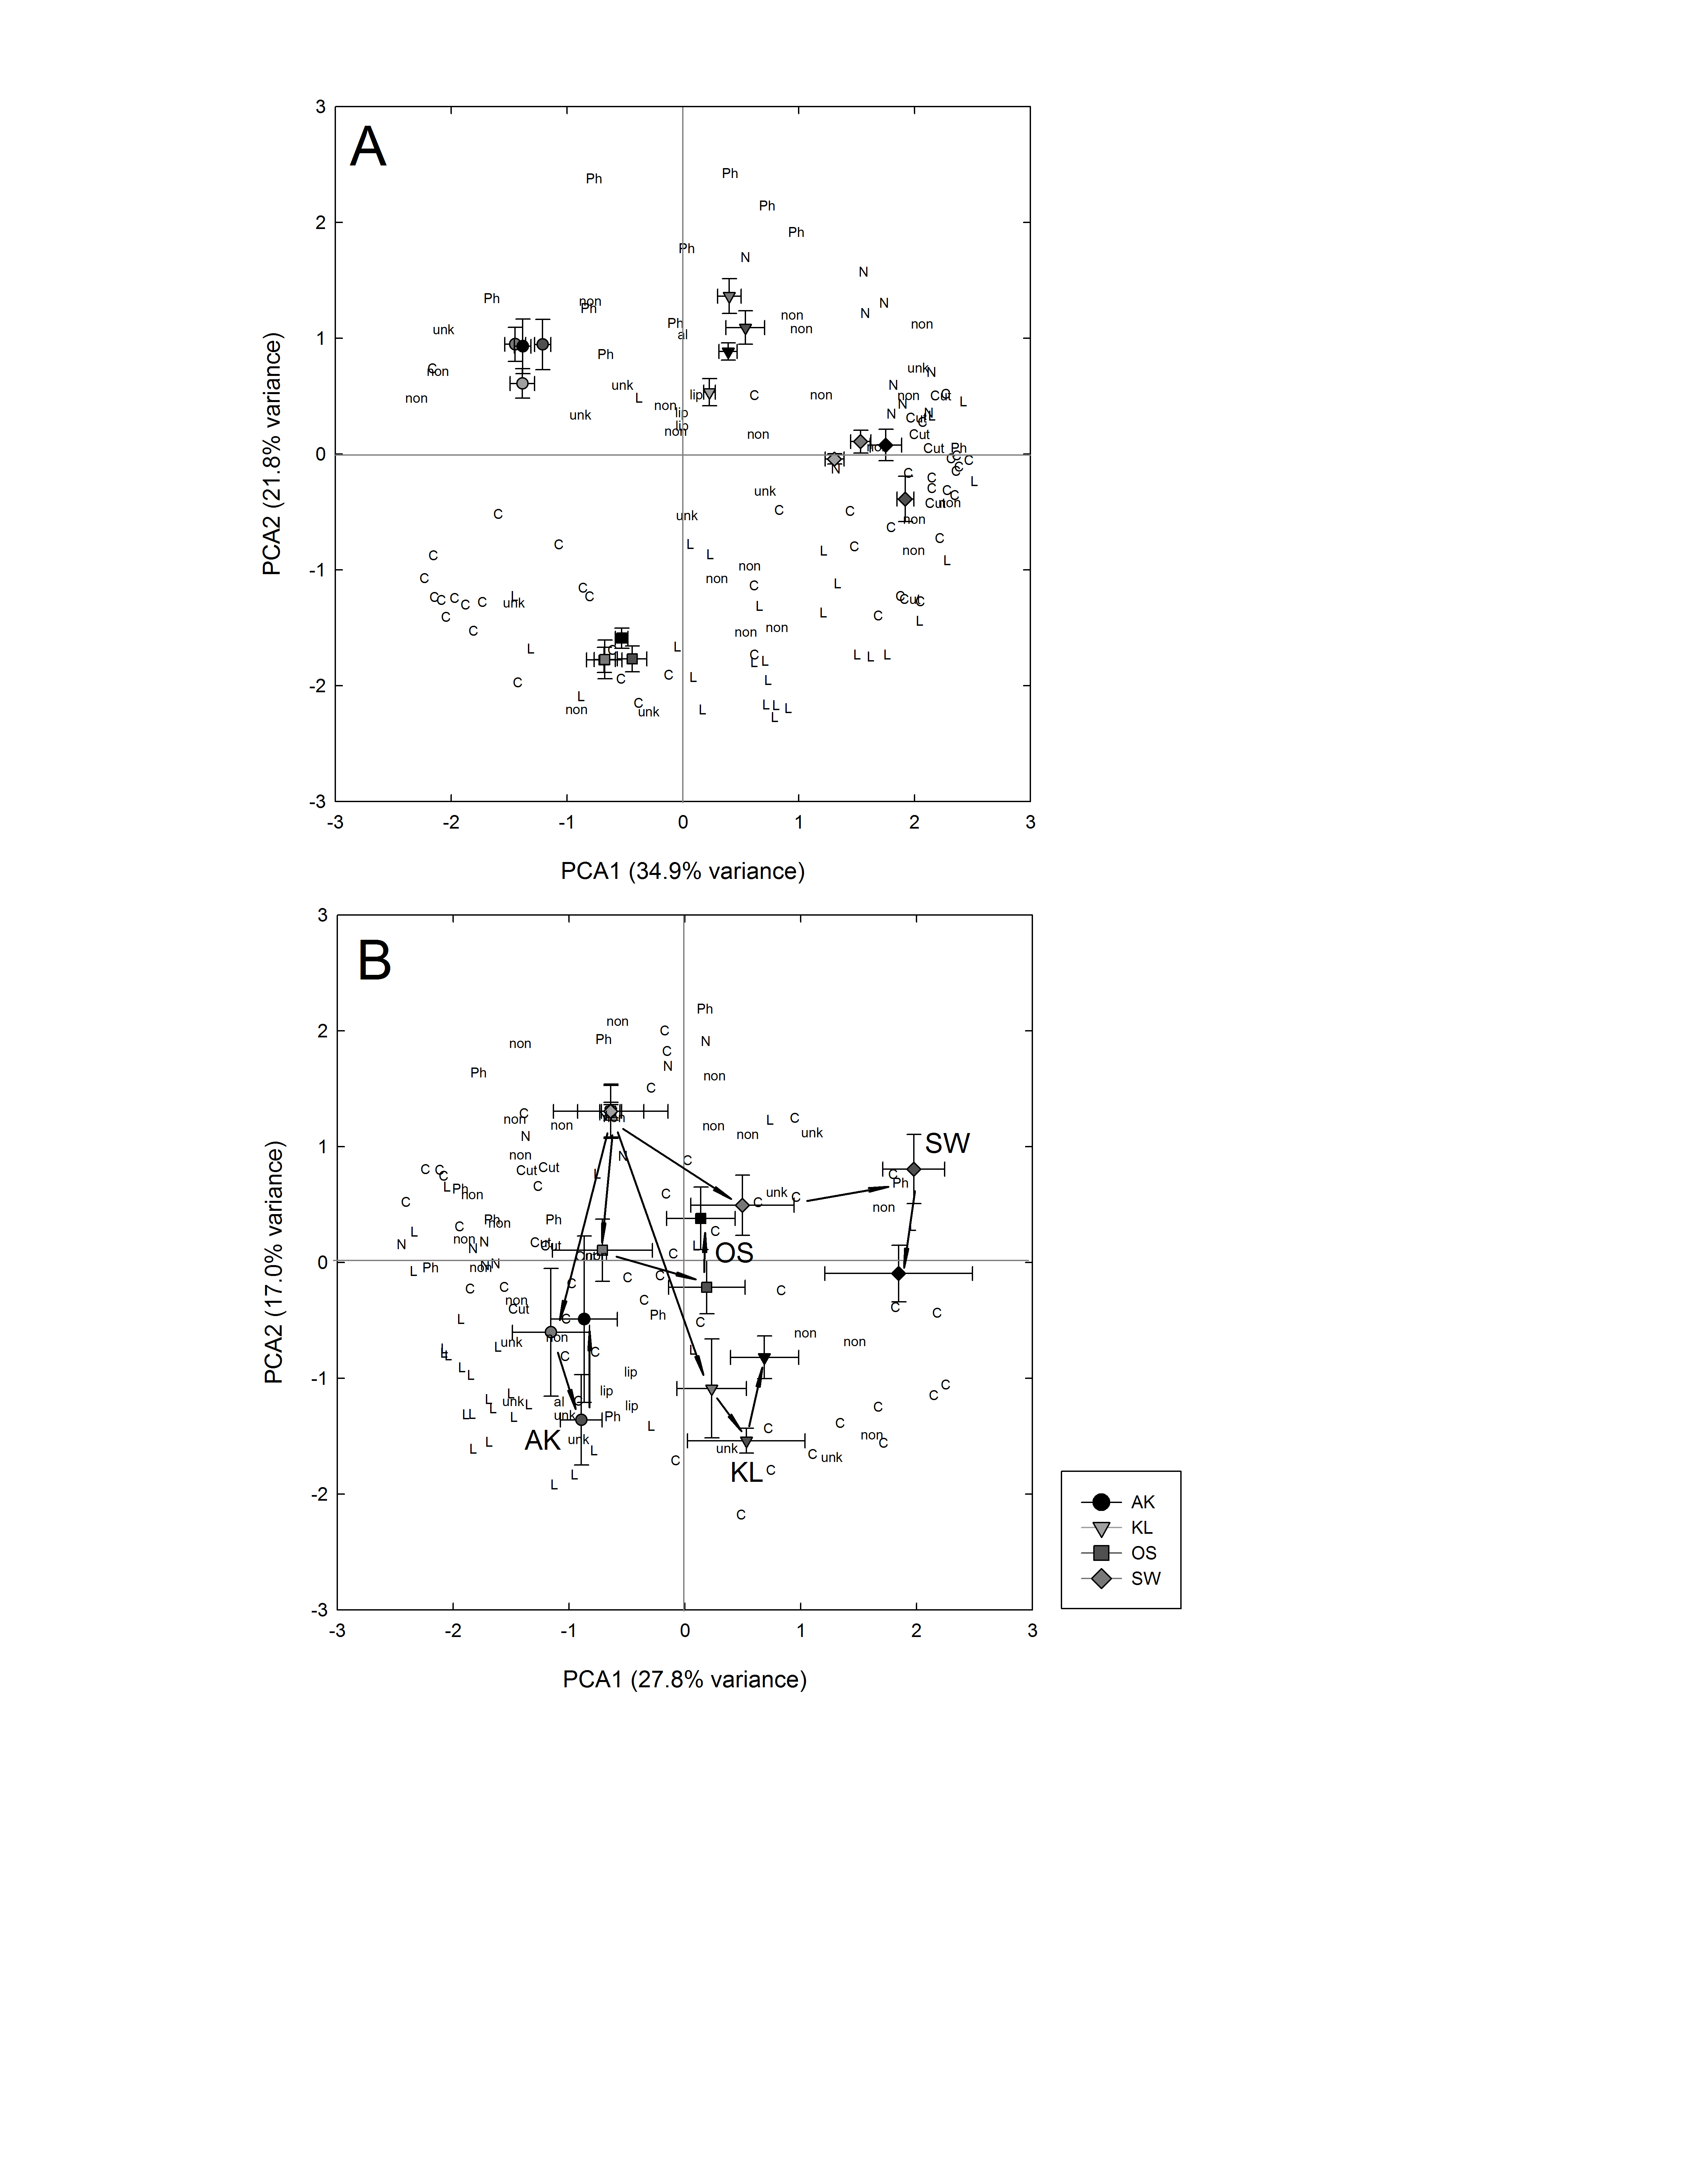
\includegraphics{fig 1+3 pca.jpg}
\end{center}
\caption{Development of the LCI (Lignin:(Lignin+Carbohydrates) and Lignin:N ratio}
\end{figure*}


\newpage
\begin{figure*}[p]
\vspace*{2mm}
\begin{center}
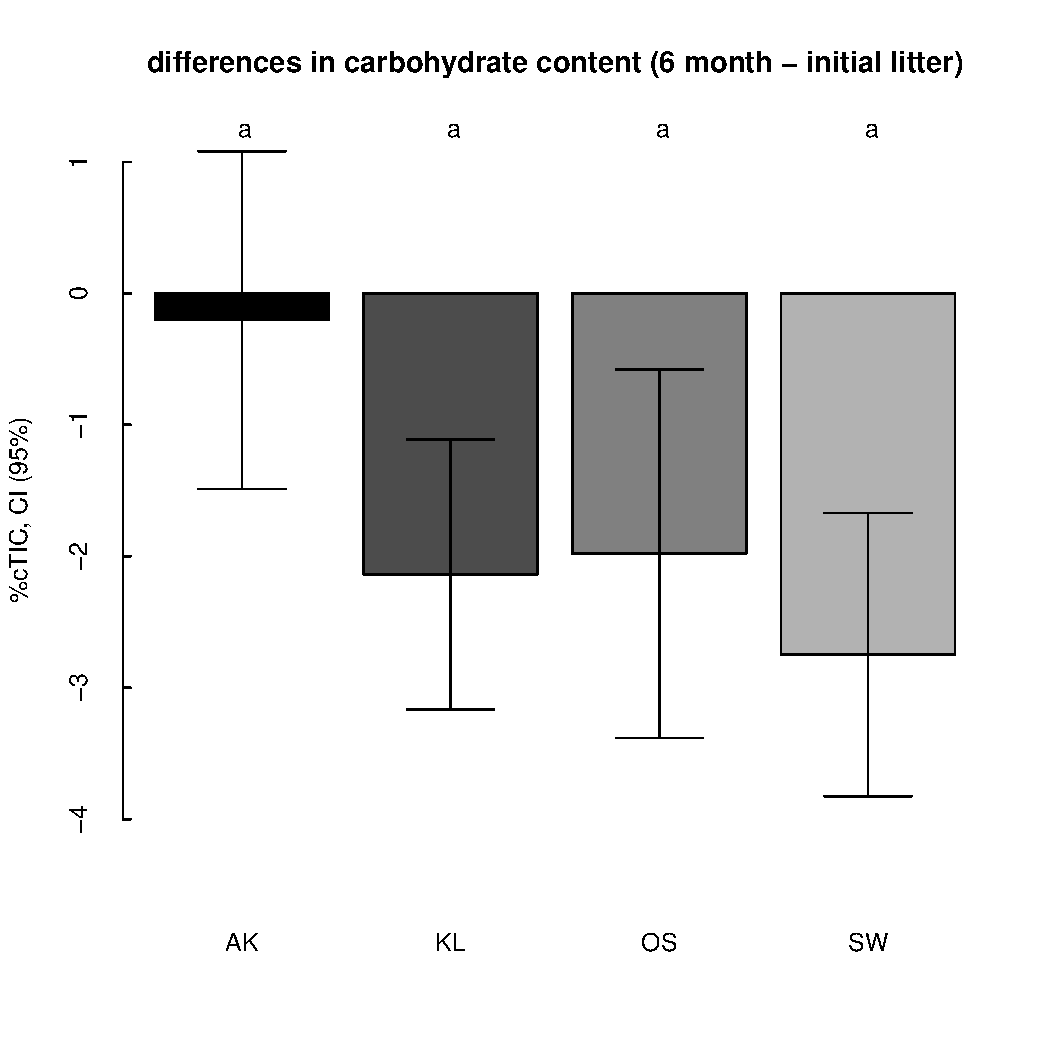
\includegraphics[width=8.3cm]{carb_differences_h3h0.pdf}
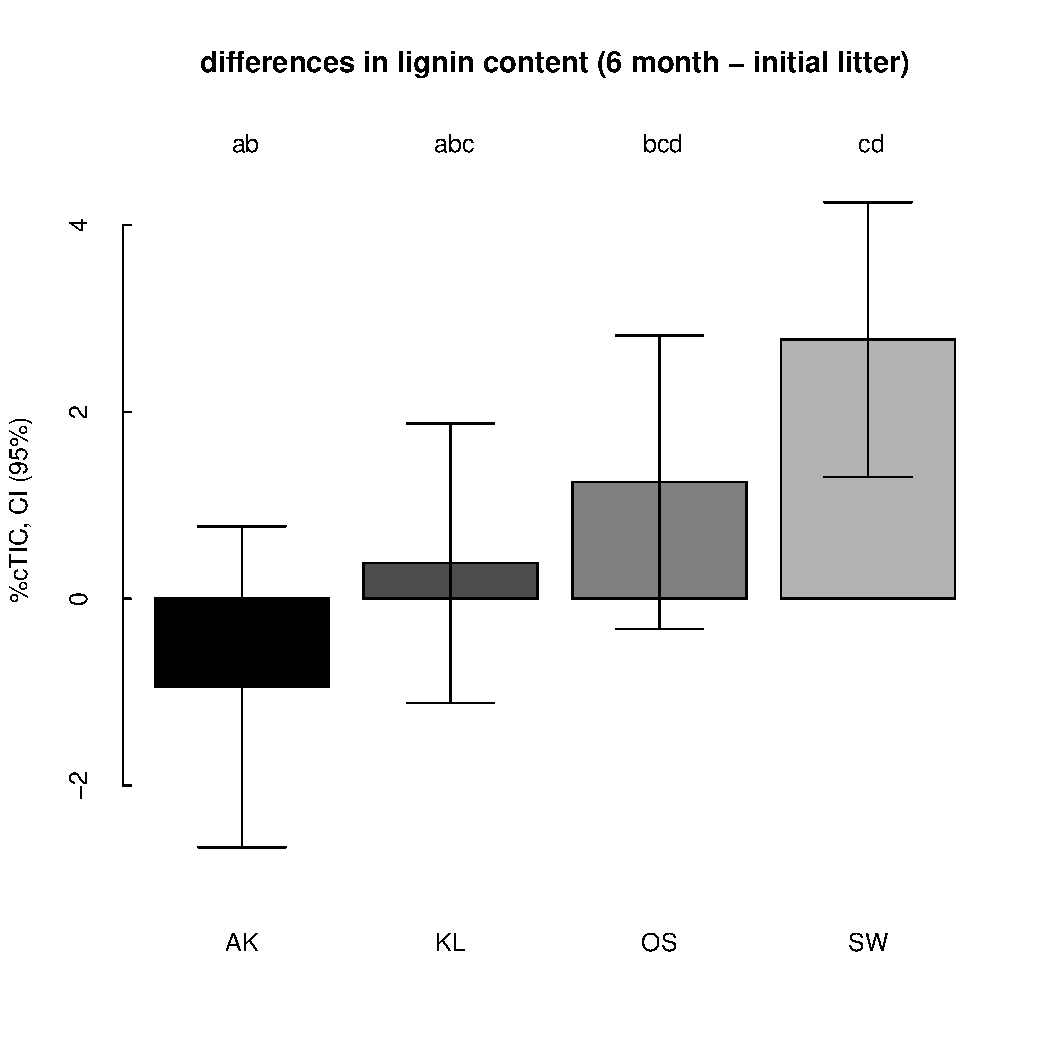
\includegraphics[width=8.3cm]{lig_differences_h3h0.pdf}
\end{center}
\caption{Difference in \% cTIC (sum of lig markers). error bars indicate 95\% confidence intervall.}
\end{figure*}

% \newpage
% \begin{figure*}[p]
% b\vspace*{2mm}
% \begin{center}
% 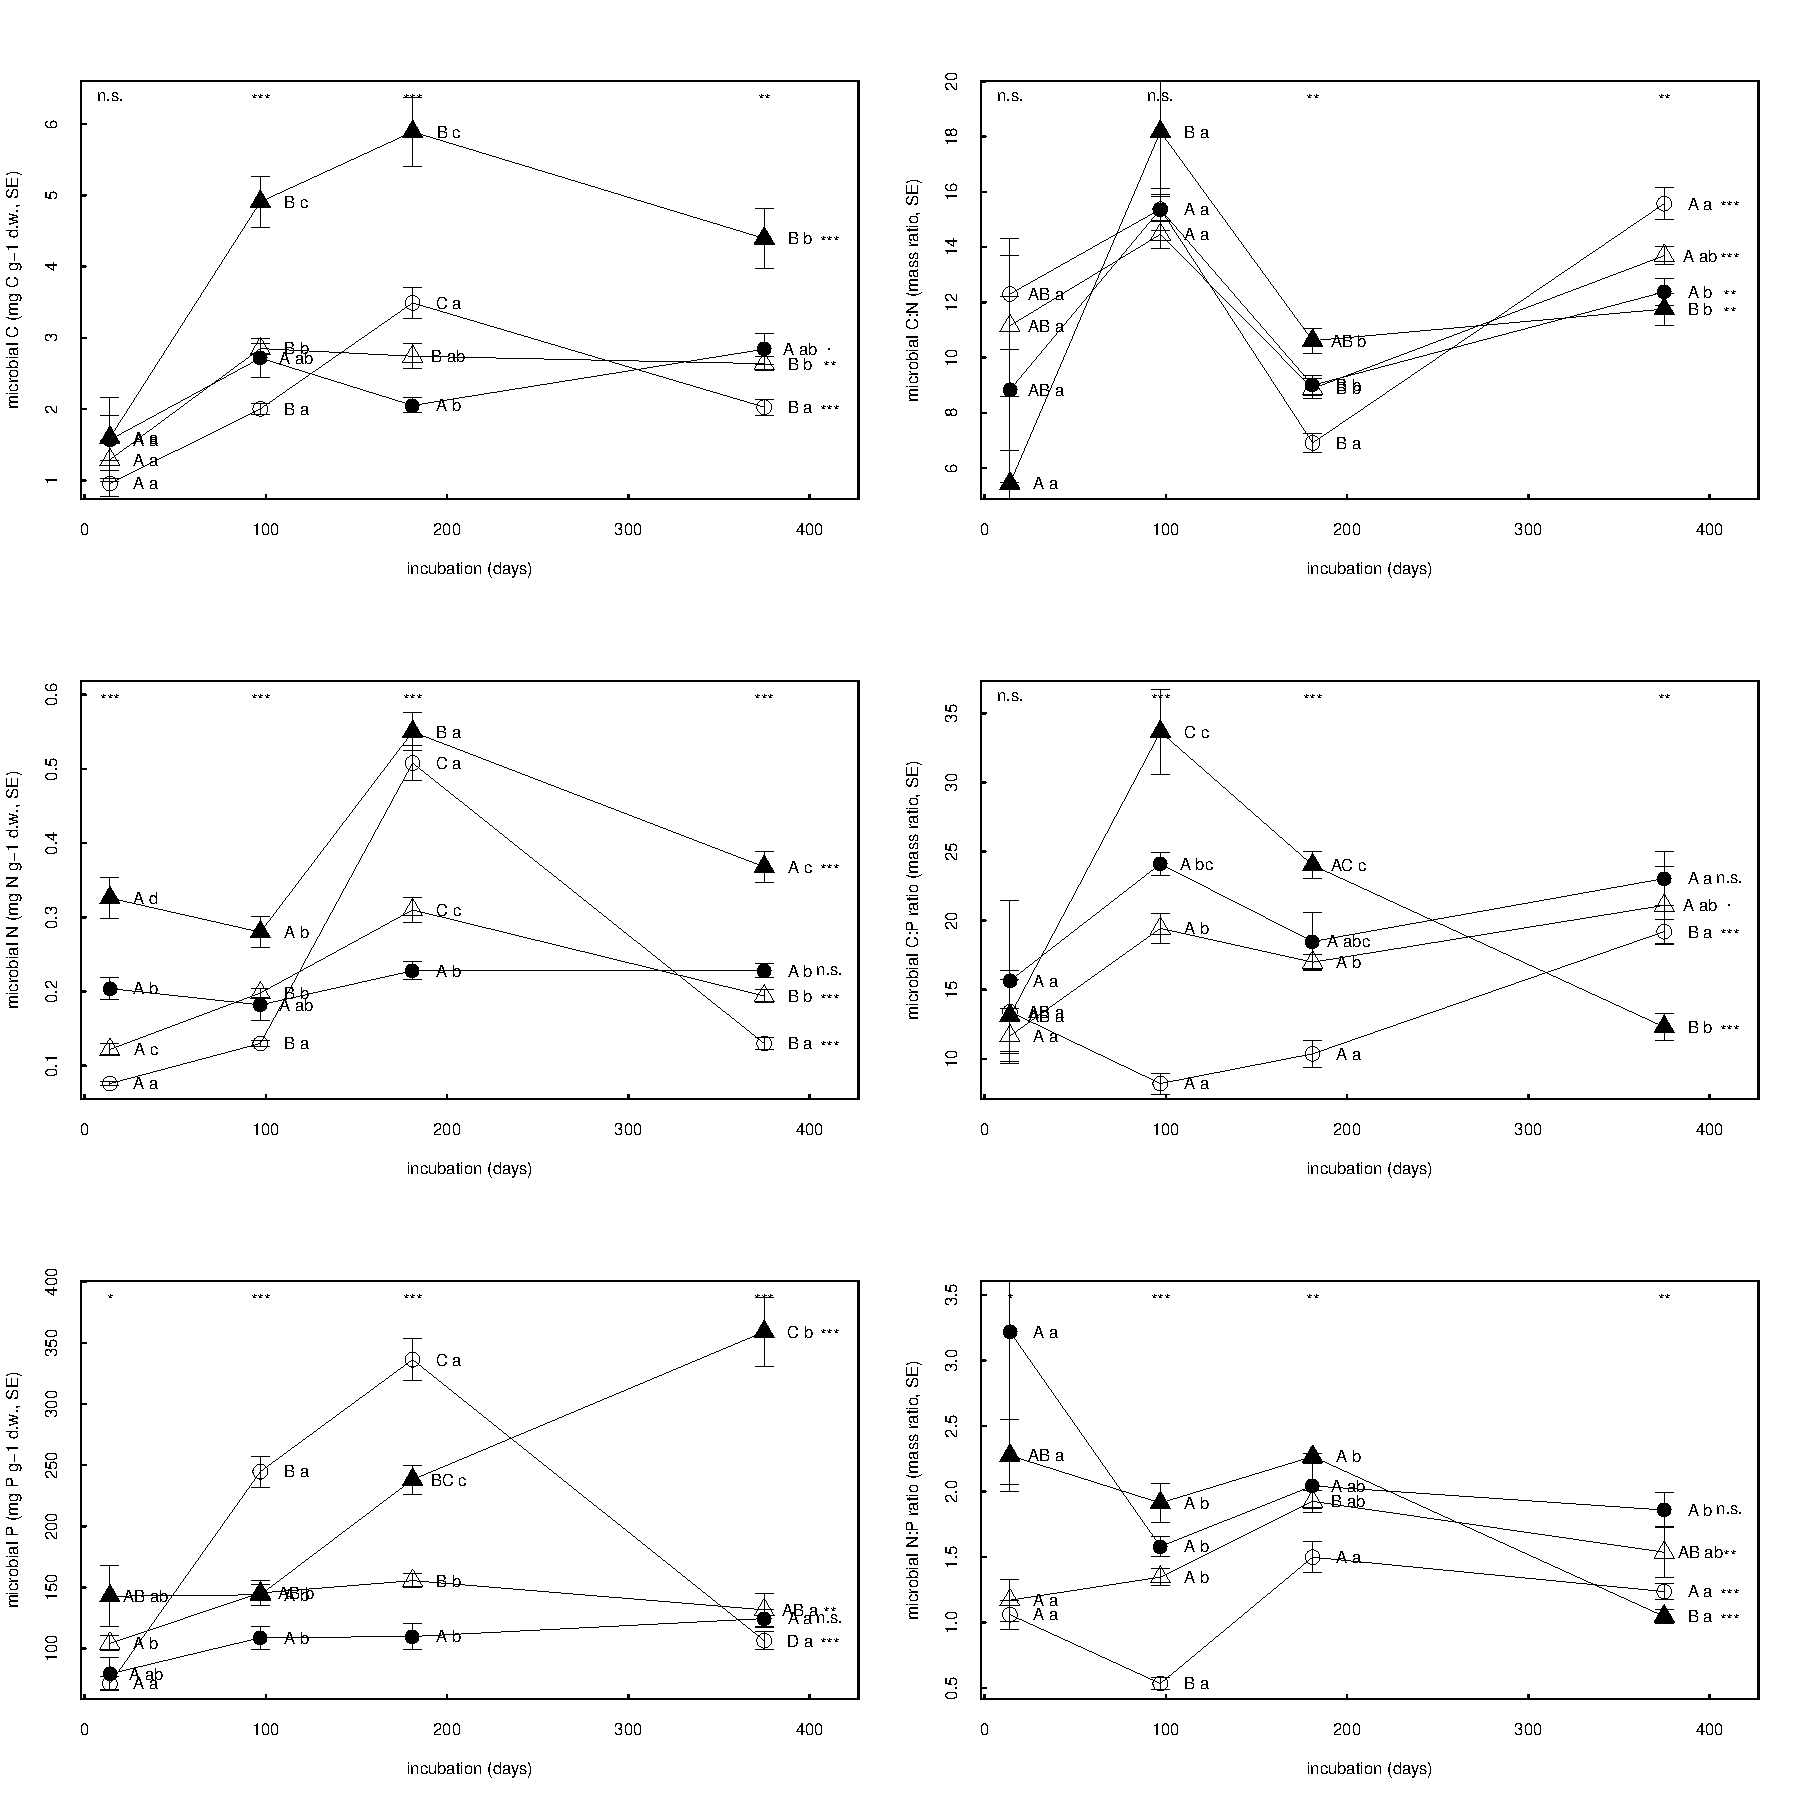
\includegraphics[width=15cm]{microbialbiomass.pdf}
% \end{center}
% \caption{Microbial C, N and P content and their ratios.}
% \end{figure*}

\newpage
\begin{figure*}[p]
\vspace*{2mm}
\begin{center}
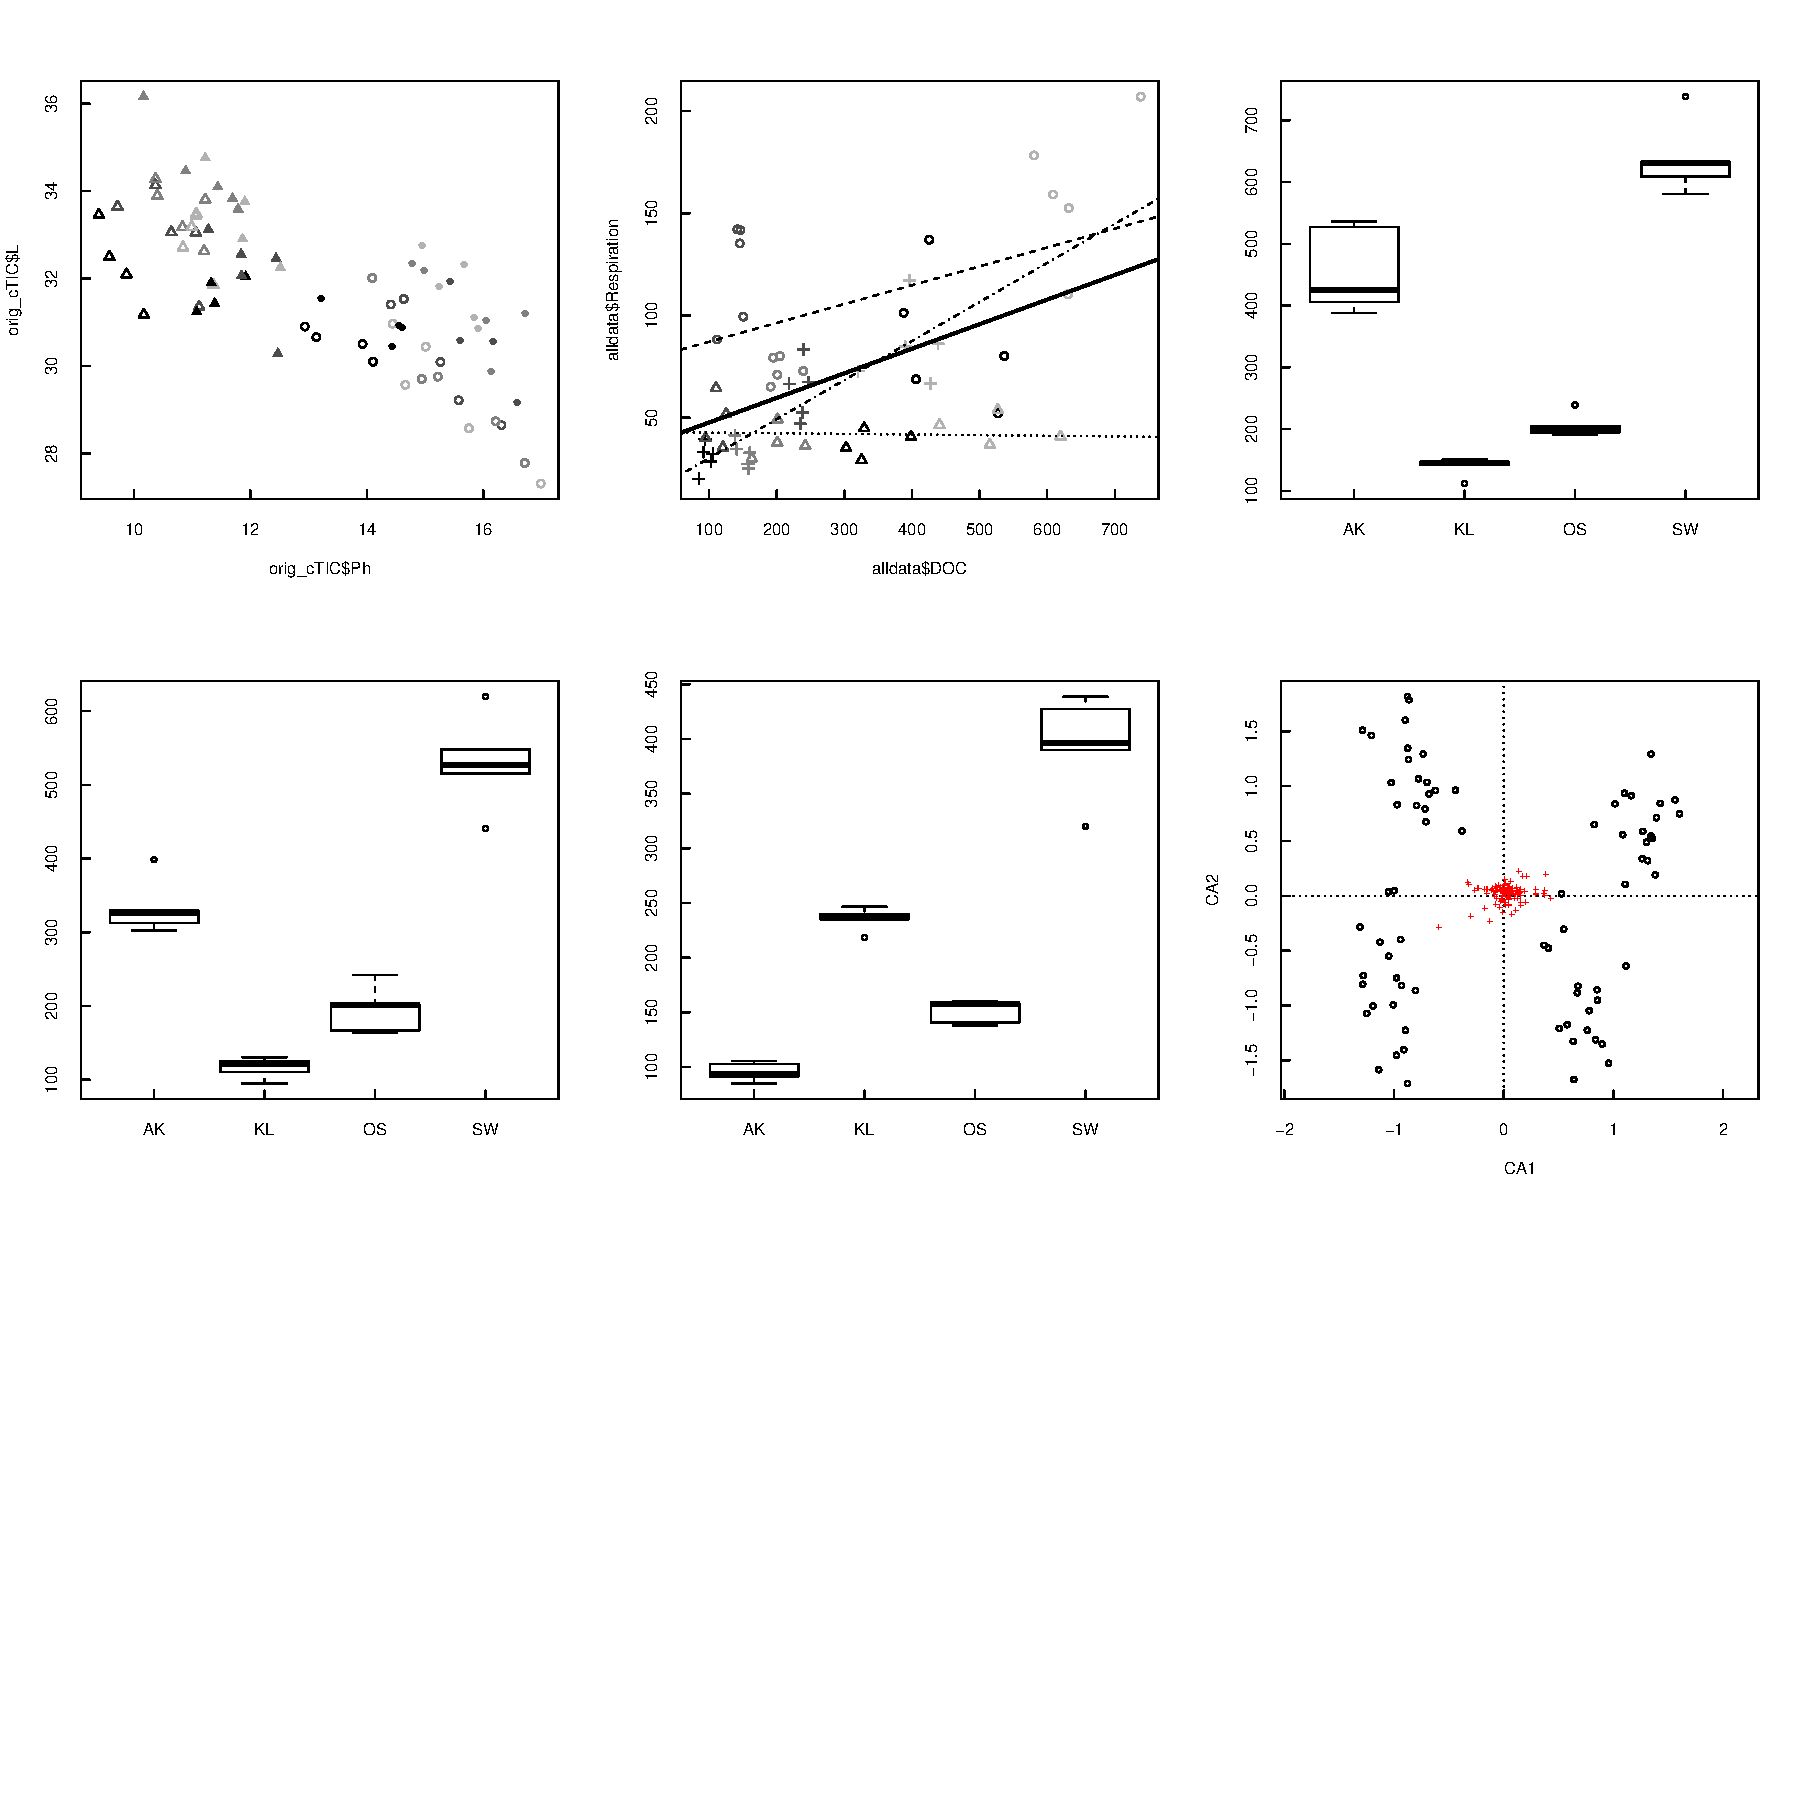
\includegraphics[width=12cm]{enzymes_barplots.pdf}
\end{center}
\caption{Potential activities of cellulase, phenoloxidase and perodase.}
\end{figure*}

\newpage
\begin{figure*}[p]
\vspace*{2mm}
\begin{center}
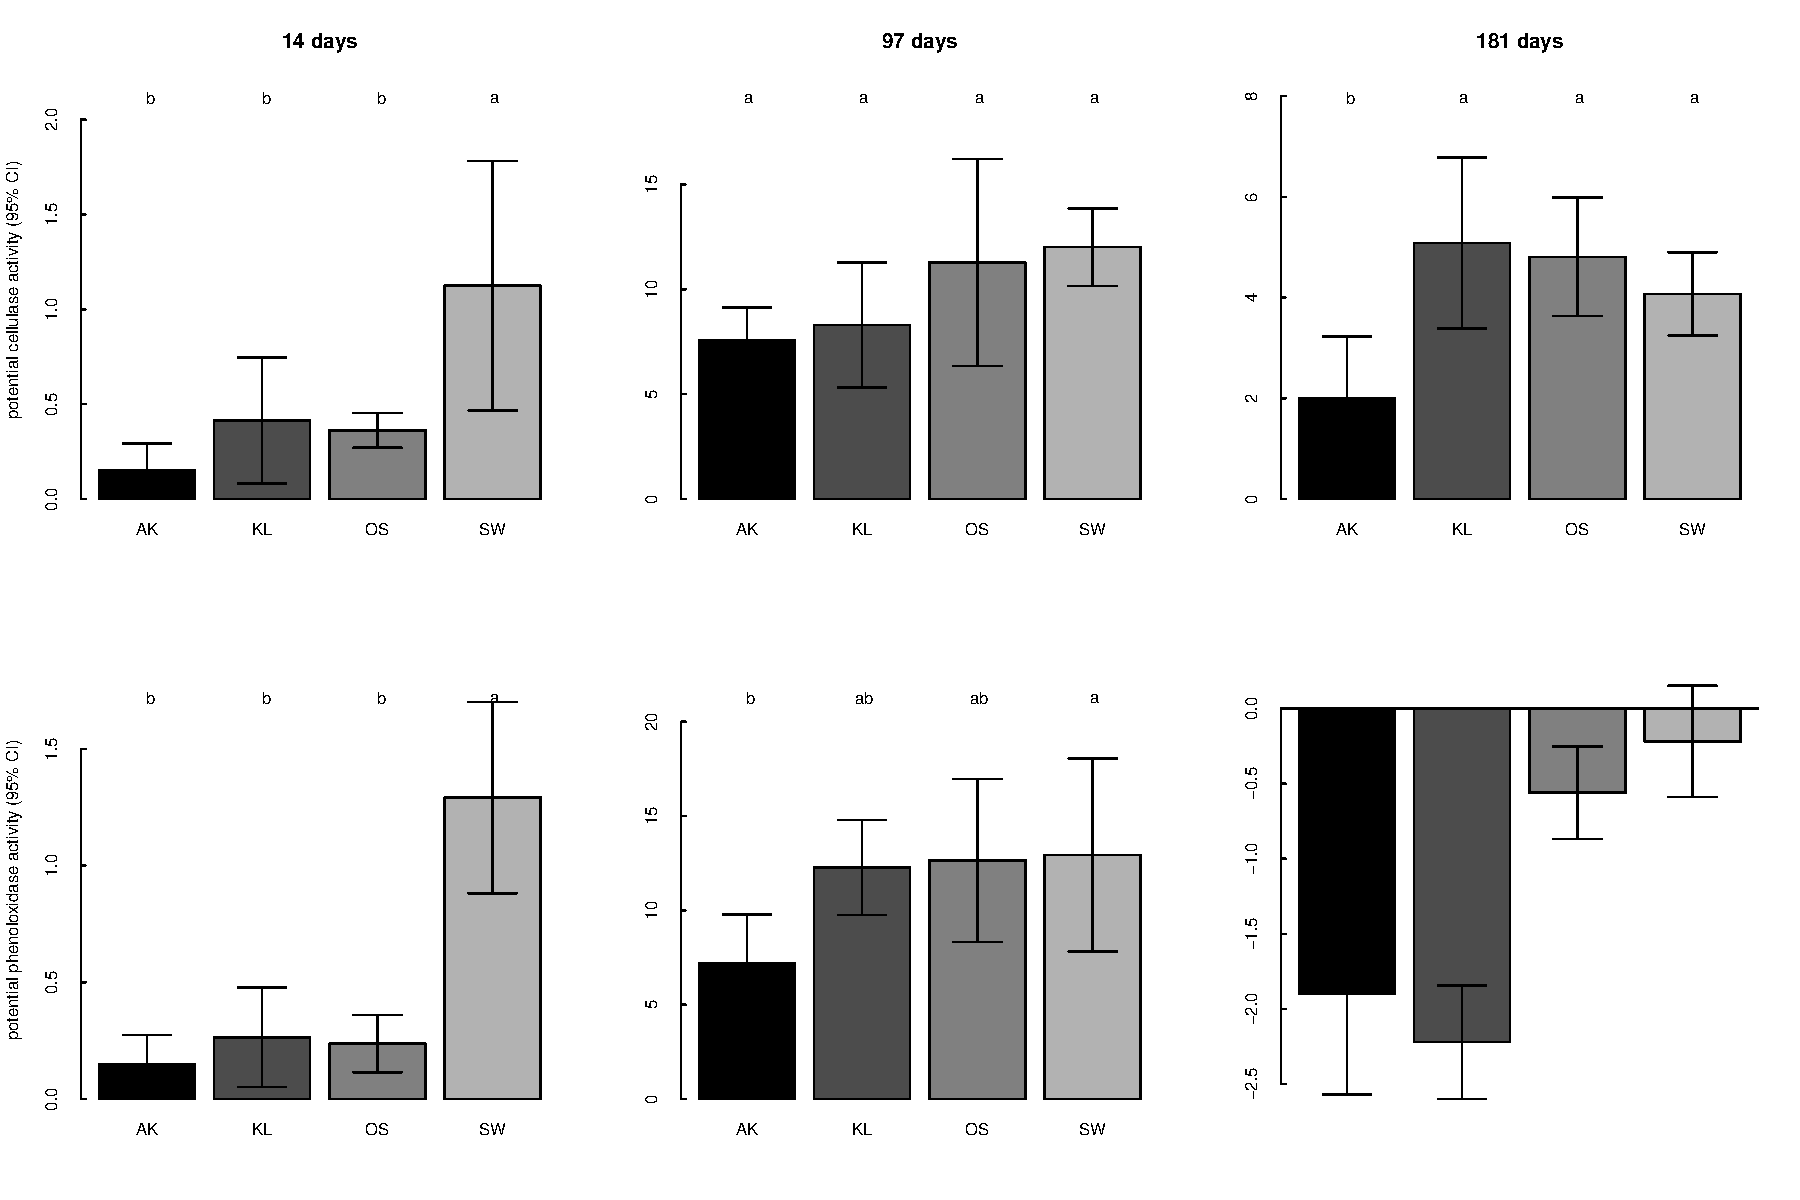
\includegraphics[width=12cm]{enzyme_ratio_barplots.pdf}
\end{center}
\caption{Ratio between cellulase and two oxidative enzymes (phenolxydase and peroxydase). The two ratios are strongly correlated, oxidative enzymes are higher in AK than in other litter types.}
\end{figure*}


\newpage
\begin{figure*}[p]
\vspace*{2mm}
  \begin{center}
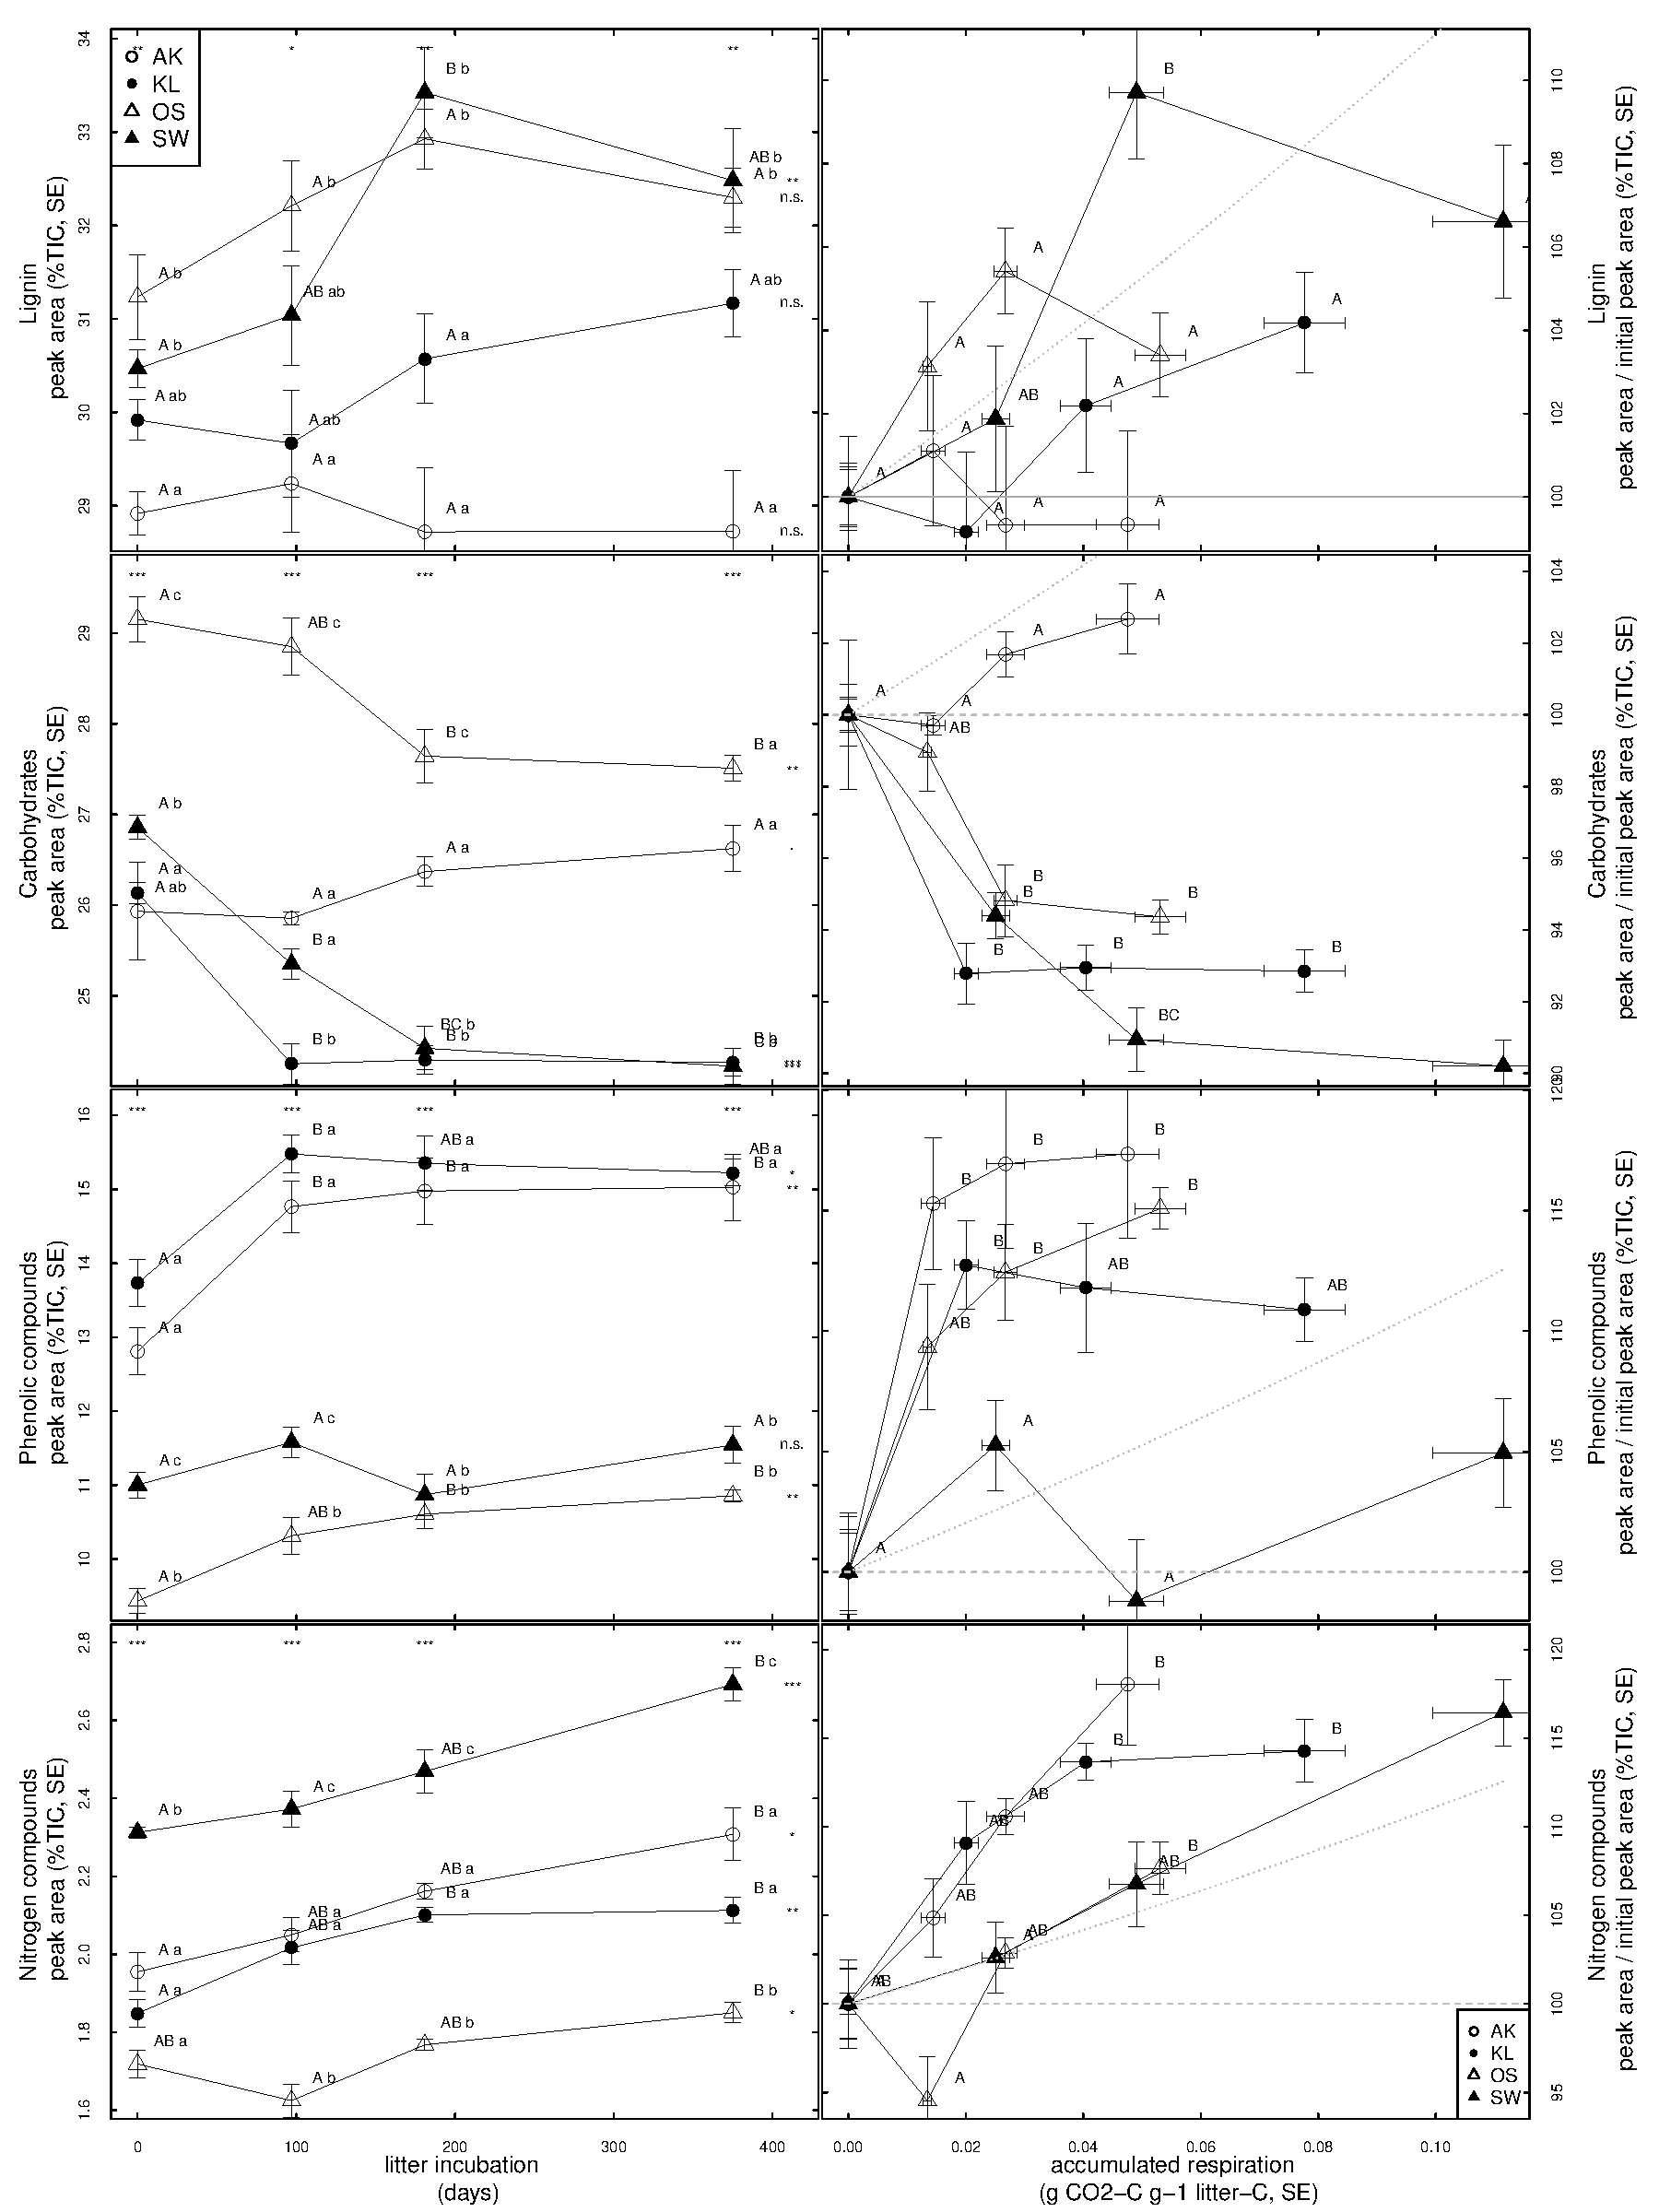
\includegraphics[width=15cm]{timeseries_orig.pdf}
%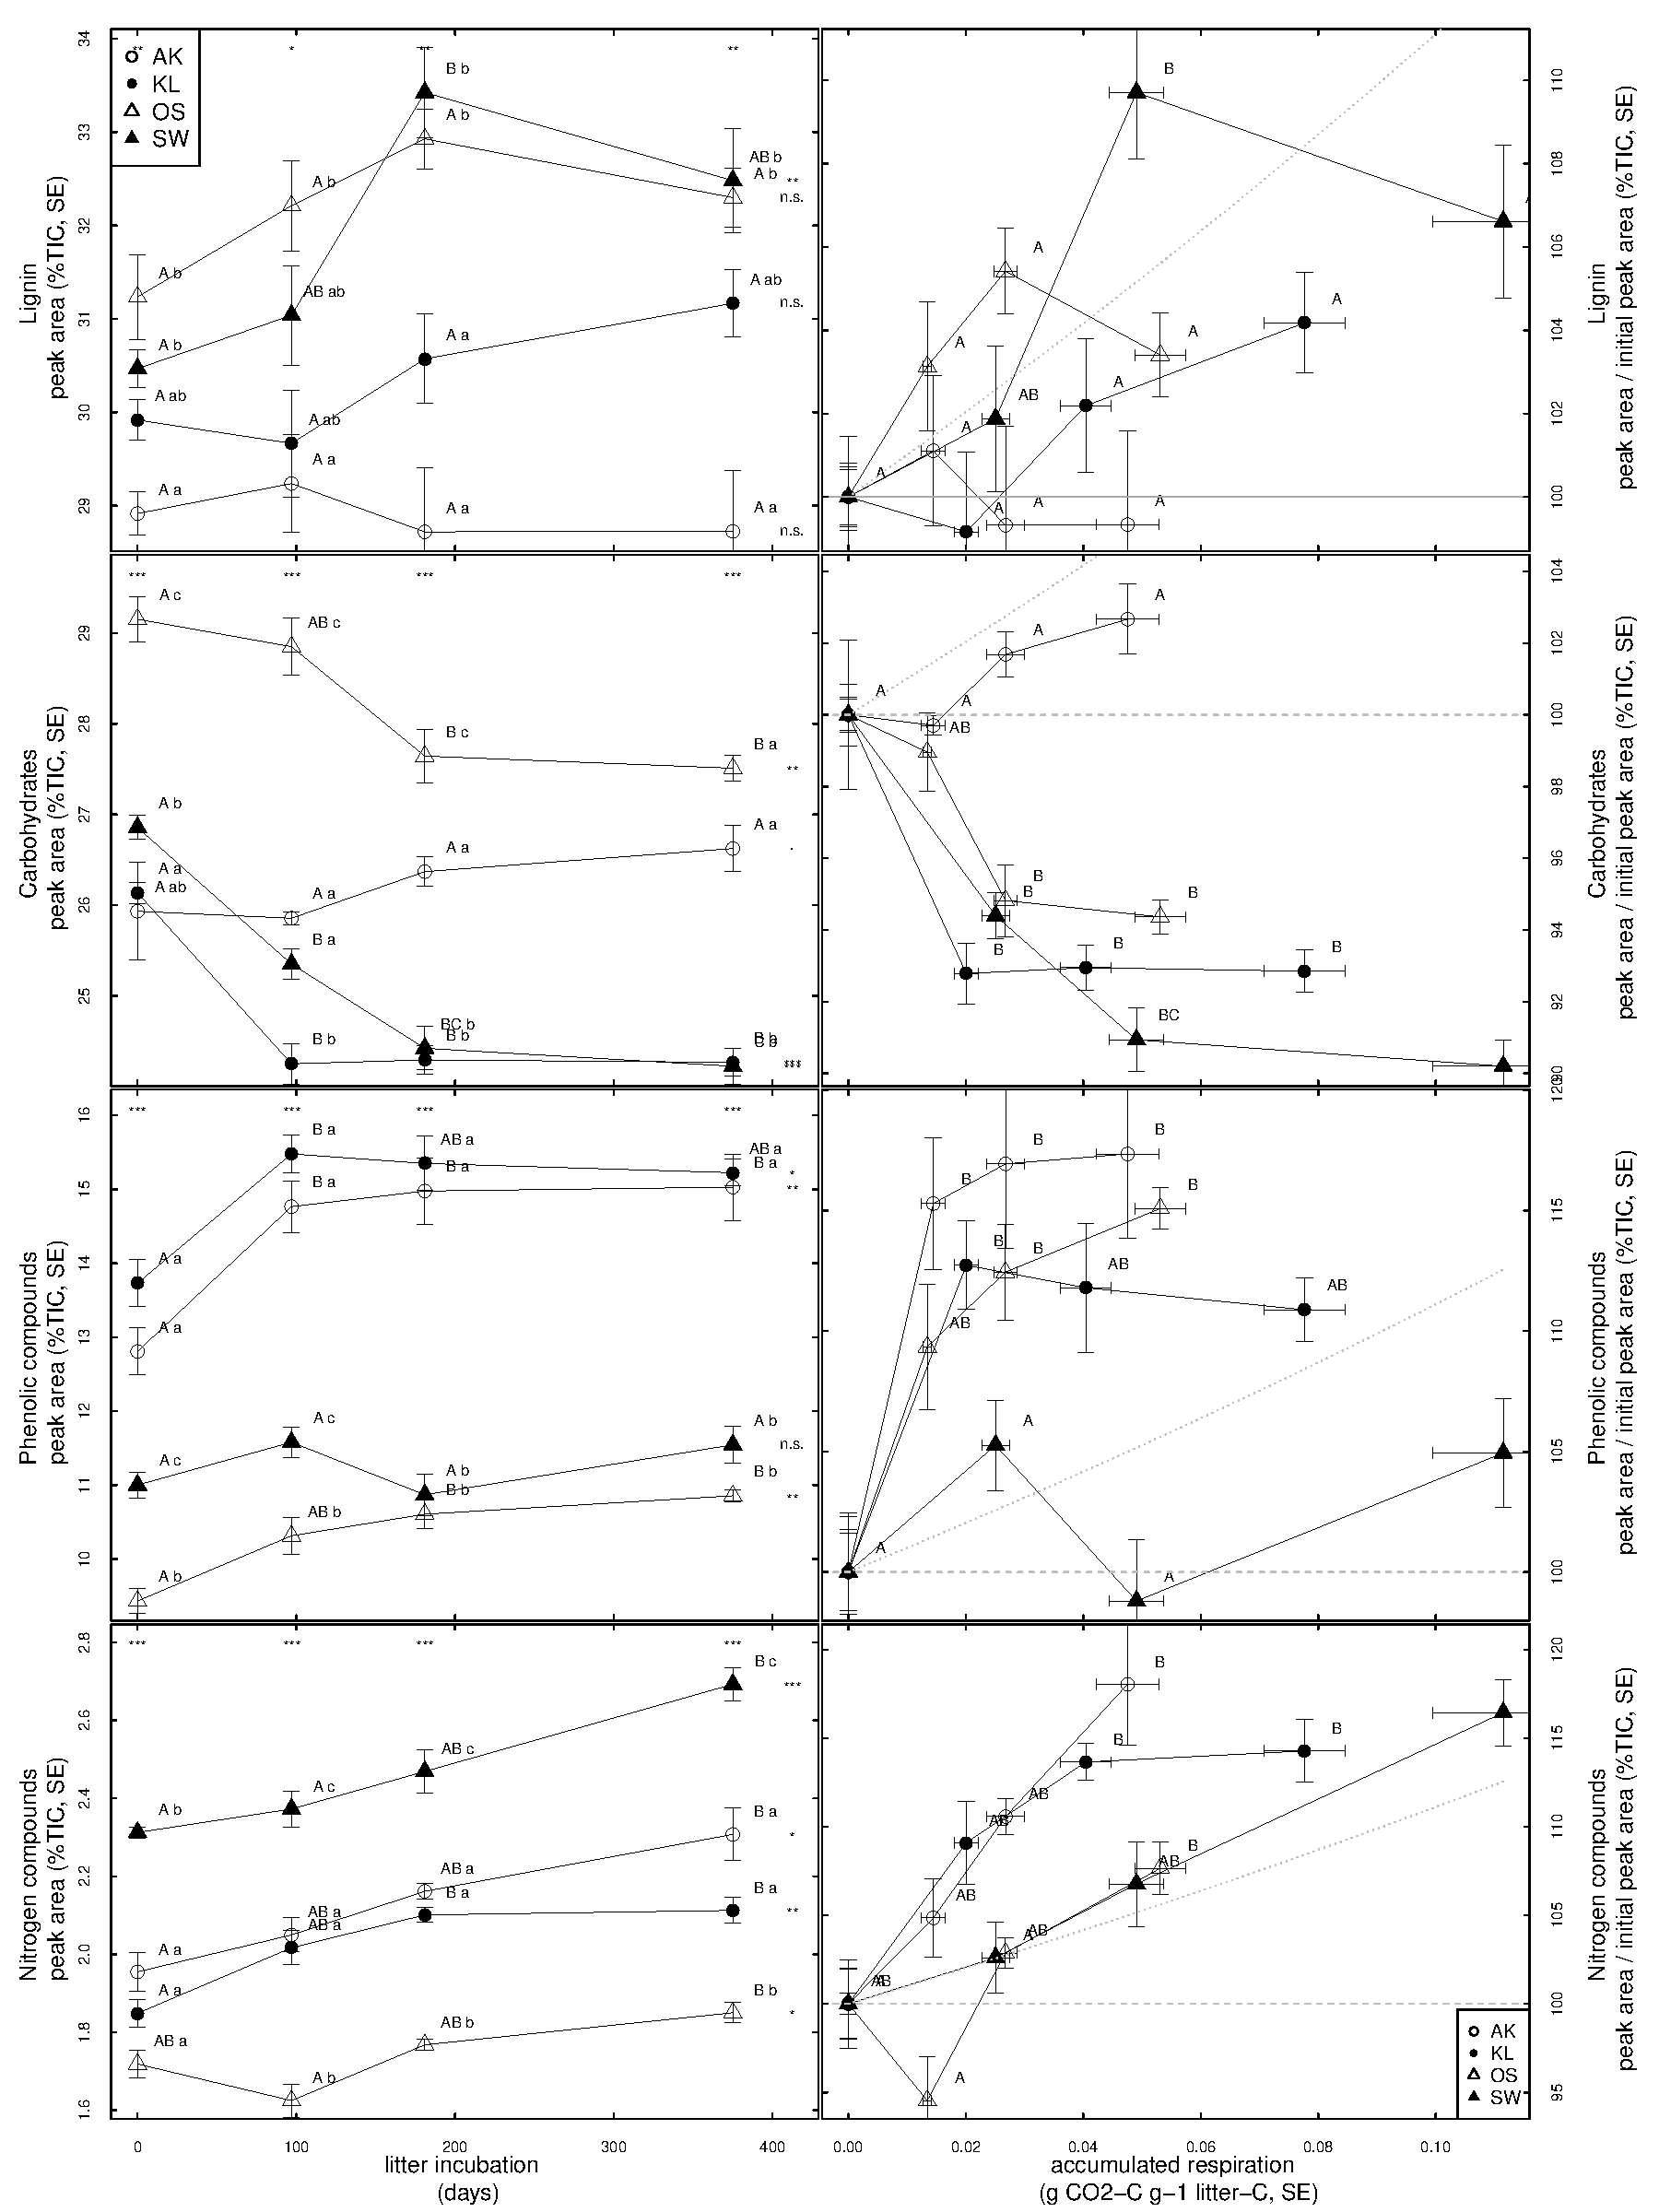
\includegraphics[width=17cm]{timeseries_orig.pdf}
\end{center}
\caption{Decomposition dynamics of HMW compound classes}
\end{figure*}

\newpage 
\begin{figure*}[p]
\vspace*{2mm}
  \begin{center}
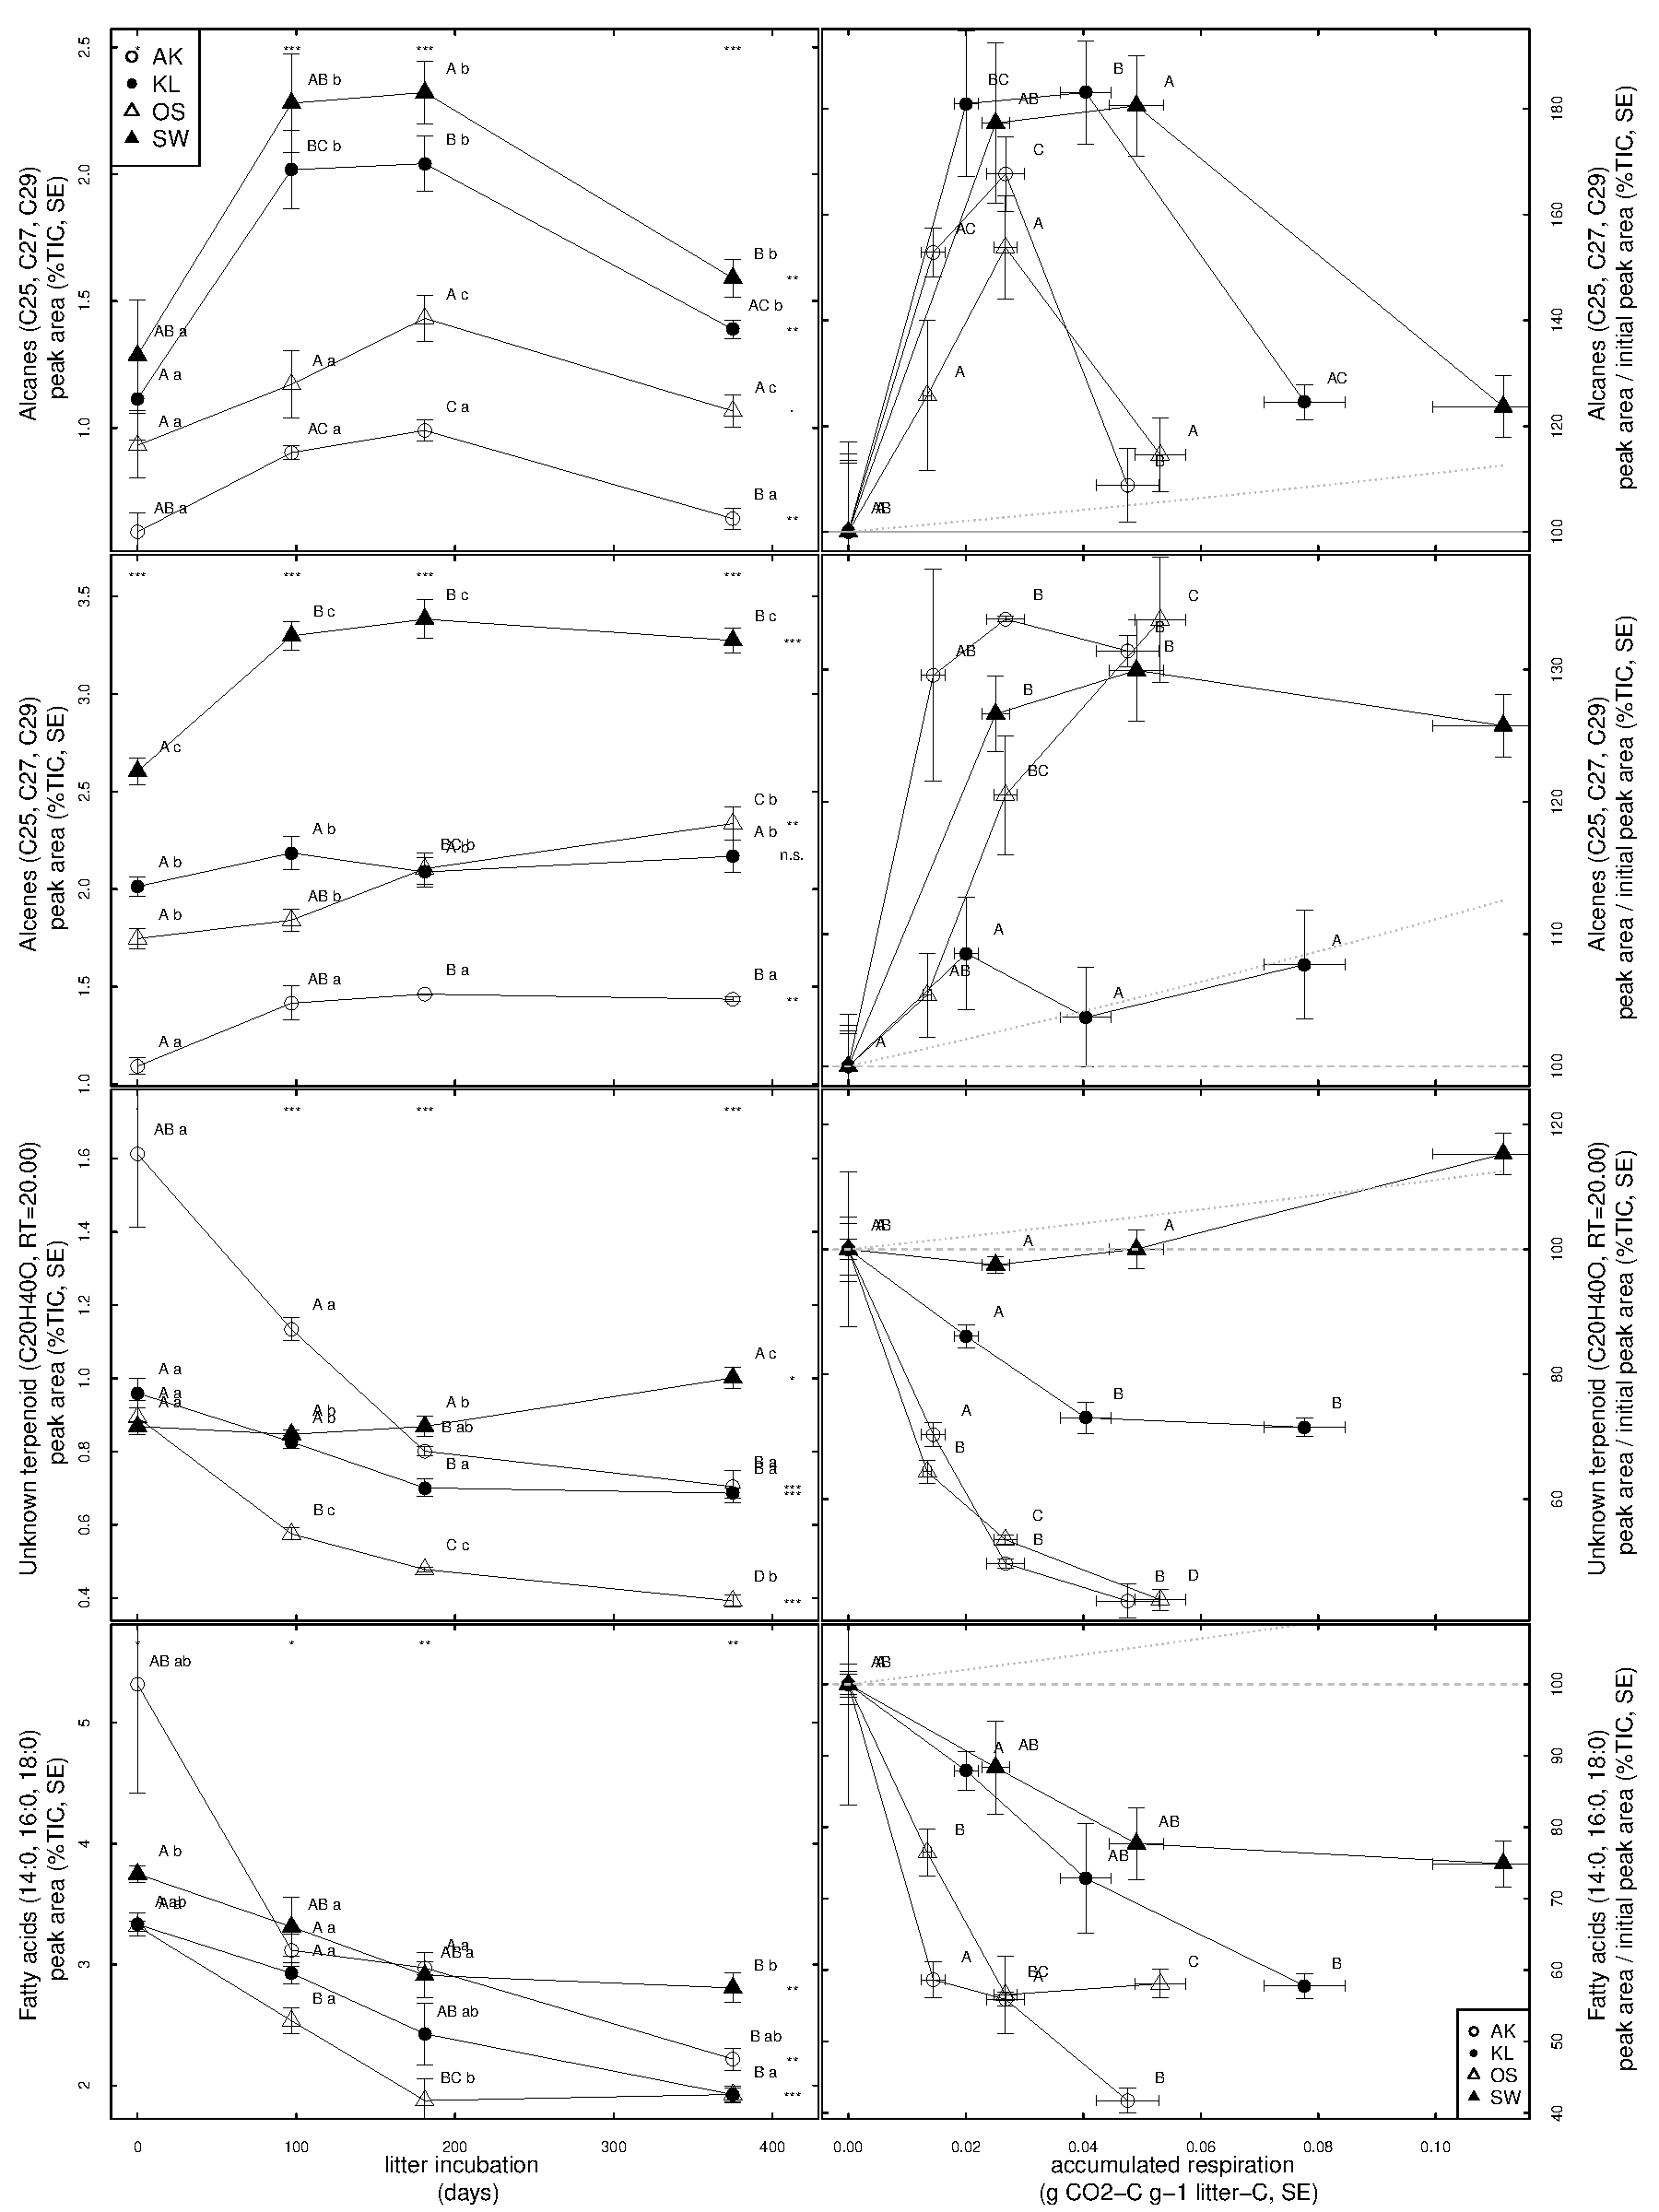
\includegraphics[width=15cm]{timeseries_waxes.pdf}
%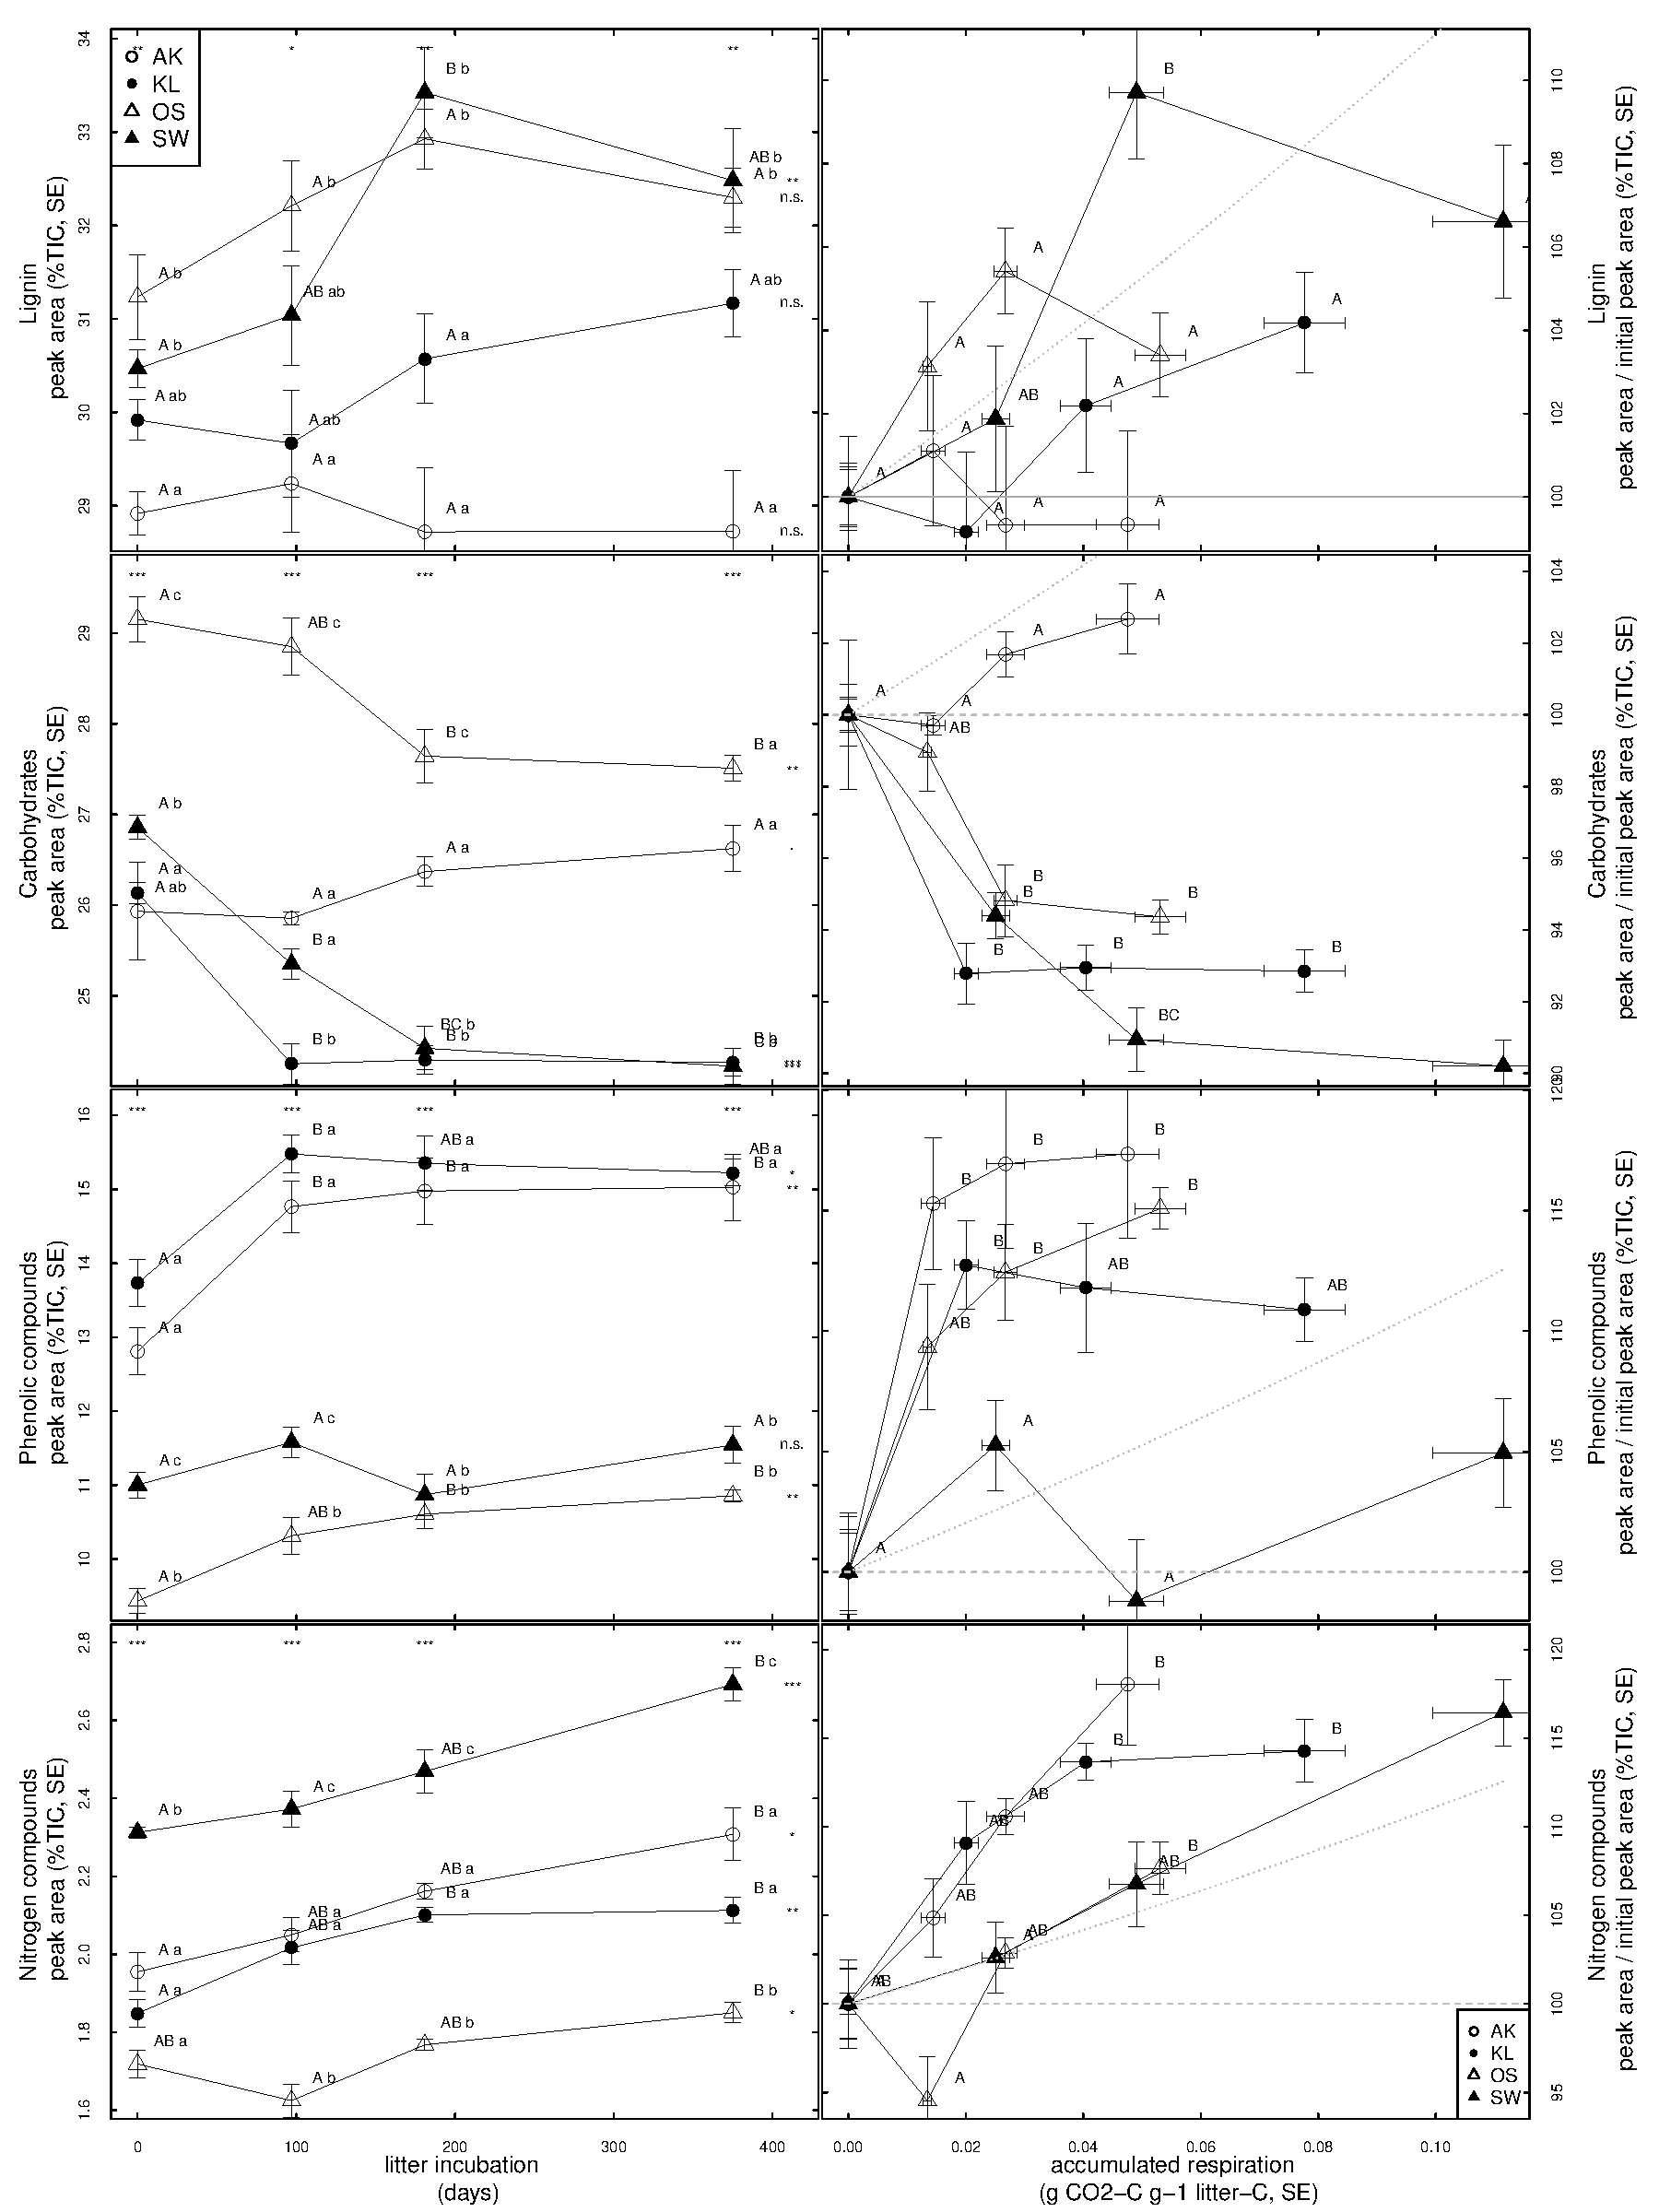
\includegraphics[width=17cm]{timeseries_orig.pdf}
\end{center}
\caption{Decomposition dynamics of lipophilic compound classes}
\end{figure*}


\newpage
\begin{figure*}[p]
\vspace*{2mm}
\begin{center}
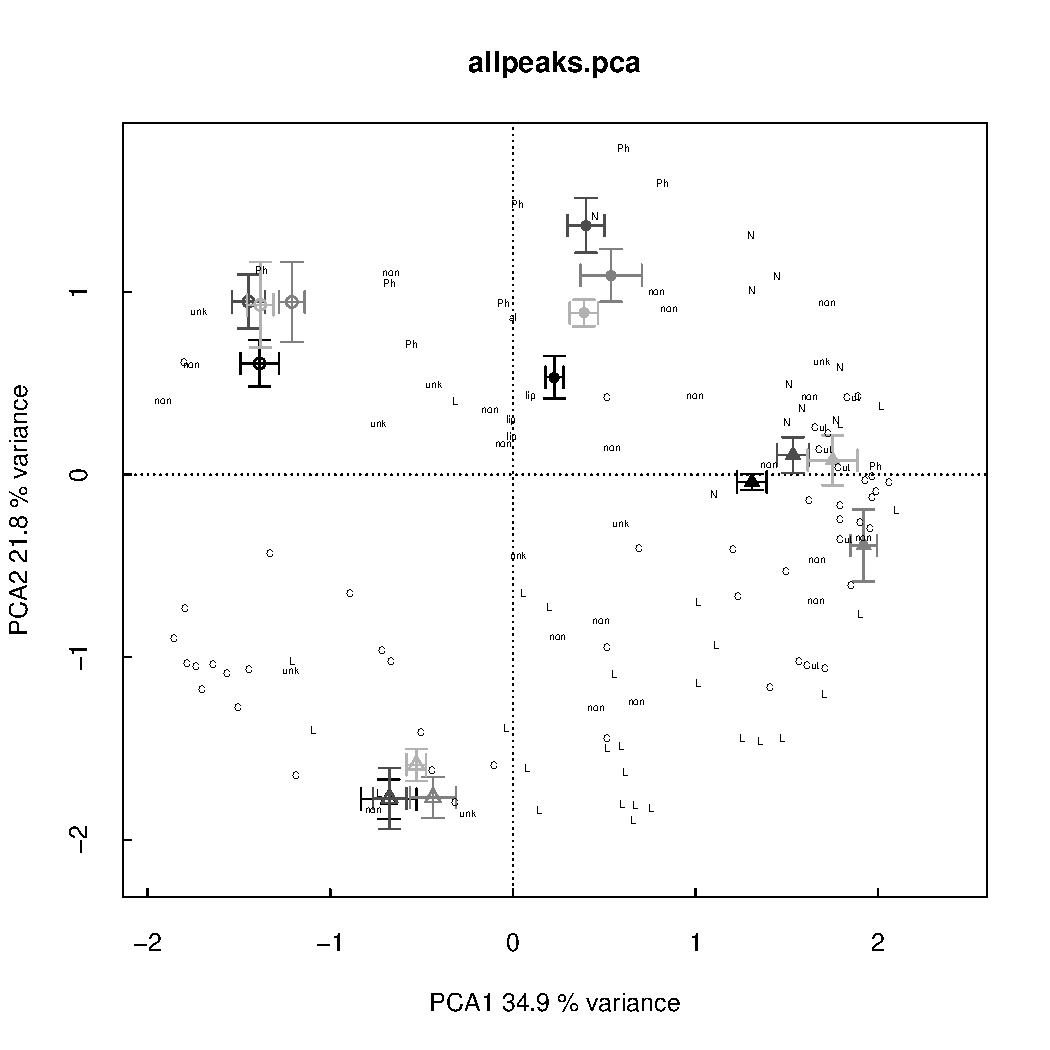
\includegraphics[width=15cm]{allpeaks_PCA12.pdf}
%\includegraphics[width=10cm]{allpeaks_allharvests_PCA34.pdf}
\end{center}
\caption{PCA of relative abundances of all 125 pyrolysis products. Open circles - AK, full circles - KL, open triangles - OS, full triangles - SW. black to light grey: harvest 0, 2, 3, and 4. Errorbars indicate 1 SE (n=4-5).}
\end{figure*}

\newpage
\begin{figure*}[p]
\vspace*{2mm}
\begin{center}
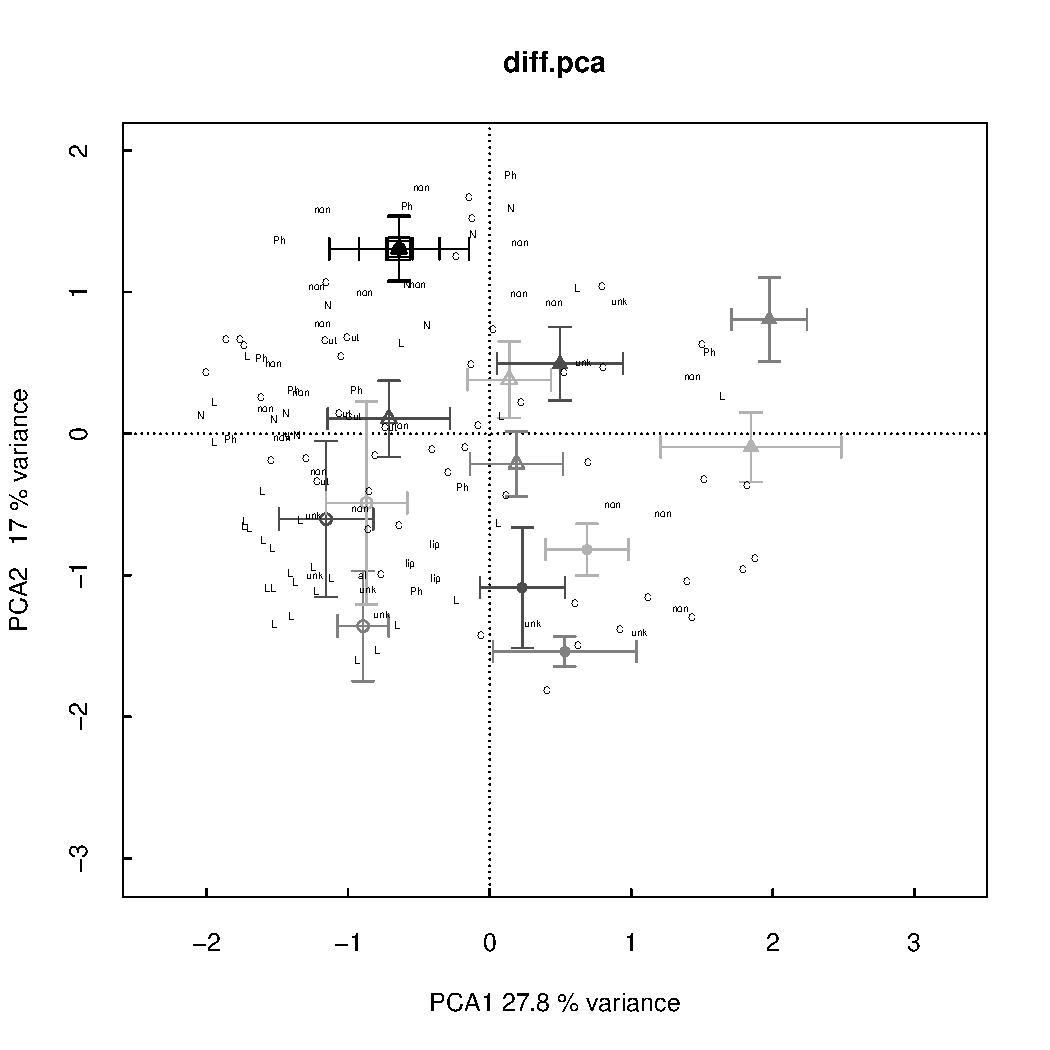
\includegraphics[width=15cm]{allpeaks_diffs_PCA12.pdf}
\end{center}
\caption{PCA of relative abundances of 125 products minus the mean relative abundance of the product in initial litter of the corresponding litter type. Open circles - AK, full circles - KL, open triangles - OS, full triangles - SW. black to light grey: harvest 0, 2, 3, and 4. Errorbars indicate 1 SE (n=4-5). Decompositino trends follow PCA1 for SW and PCA2 for AK. KL and OS show mixed trends.}
\end{figure*}



% \begin{figure*}[p]
%  \vspace*{2mm}
% \begin{center}
% 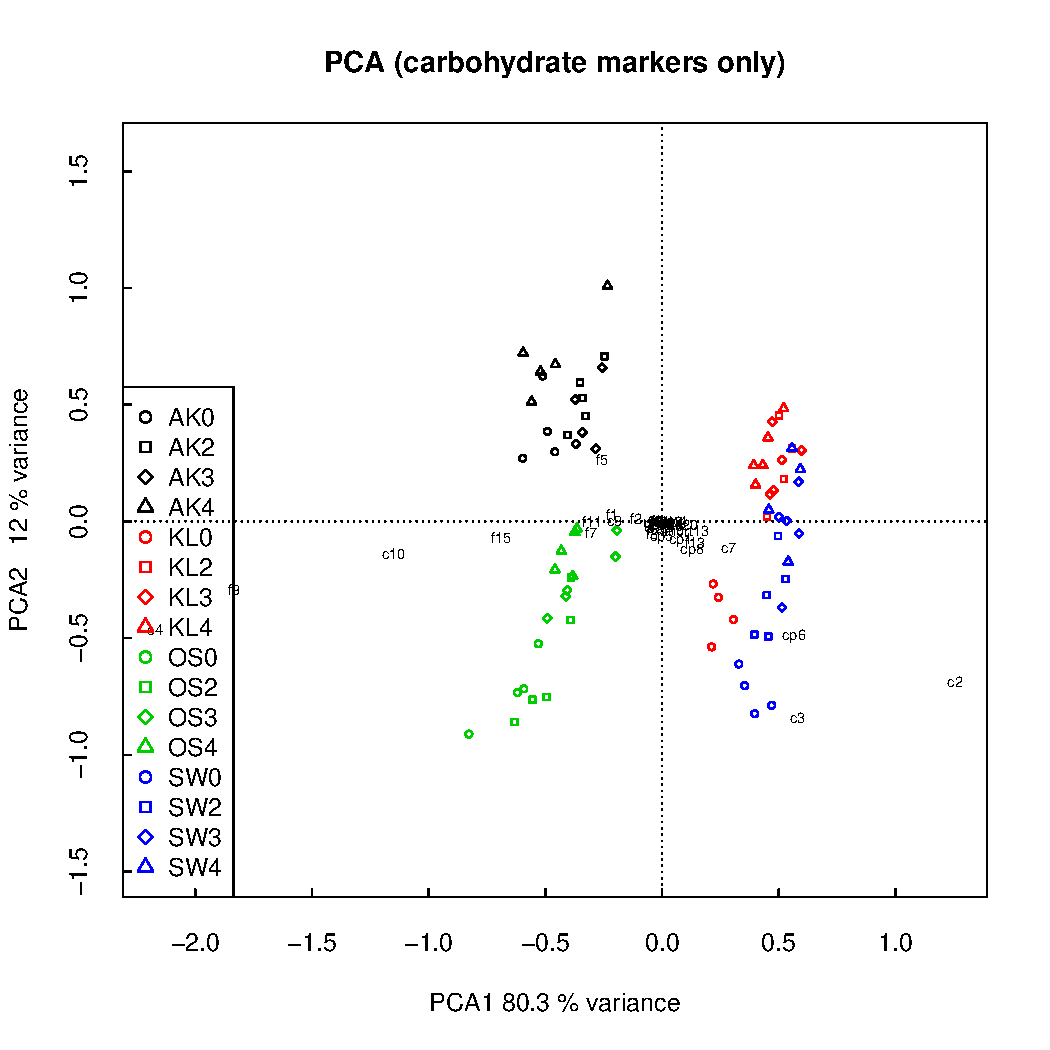
\includegraphics[width=10cm]{pca12_carbos.pdf}
% 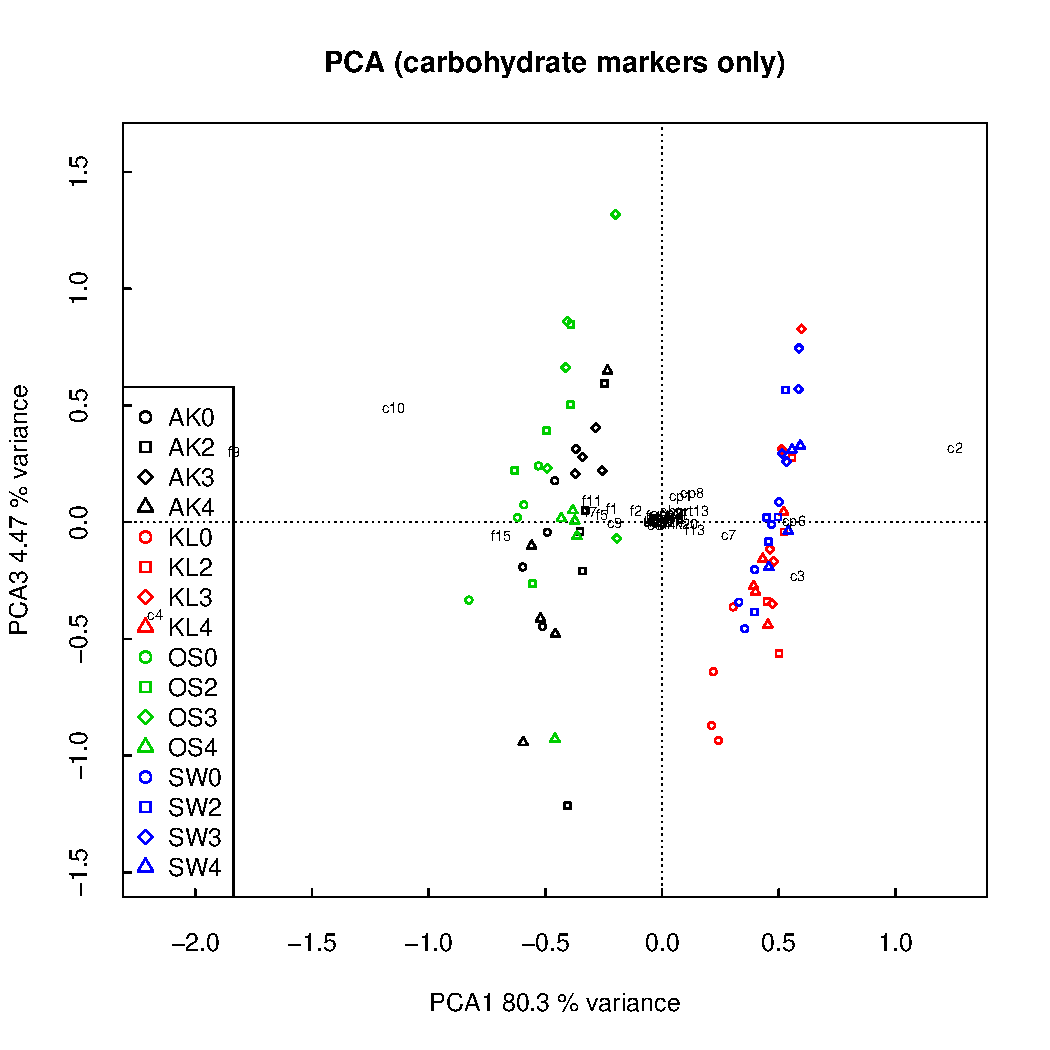
\includegraphics[width=10cm]{pca13_carbos.pdf}
% 
% \end{center}
% \caption{TEXT}
% \end{figure*}
% 
% %% TWO-COLUMN FIGURES
% 
% %f
% \begin{figure*}[p]
% \vspace*{2mm}
% \begin{center}
% \includegraphics[width=10cm]{ligonly_allharvests_PCA12.pdf}
% 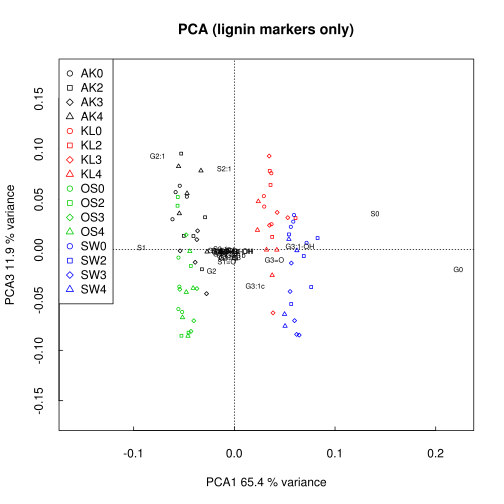
\includegraphics[width=10cm]{ligonly_allharvests_PCA13.pdf}
% \end{center}
% \caption{TEXT}
% \end{figure*}
% 

\newpage
 \begin{figure*}[p]
 \vspace*{2mm}
 \begin{center}
 \includegraphics[width=15cm]{controls_h1.pdf}
 \end{center}
 \caption{Litter chemistry: content of macro and micronutrients, 14 days after innoculation, n=5}
 \end{figure*}

% \begin{figure*}[p]
% \vspace*{2mm}
% \begin{center}
% \includegraphics[width=12cm]{controls_h2.pdf}
% \end{center}
% \caption{Litter chemistry: content of macro and micronutrients, 97 days after innoculation, n=5}
% \label{fig:litchem_h2}% \end{figure*}

\newpage
\begin{figure*}[p]
\vspace*{2mm}
\begin{center}
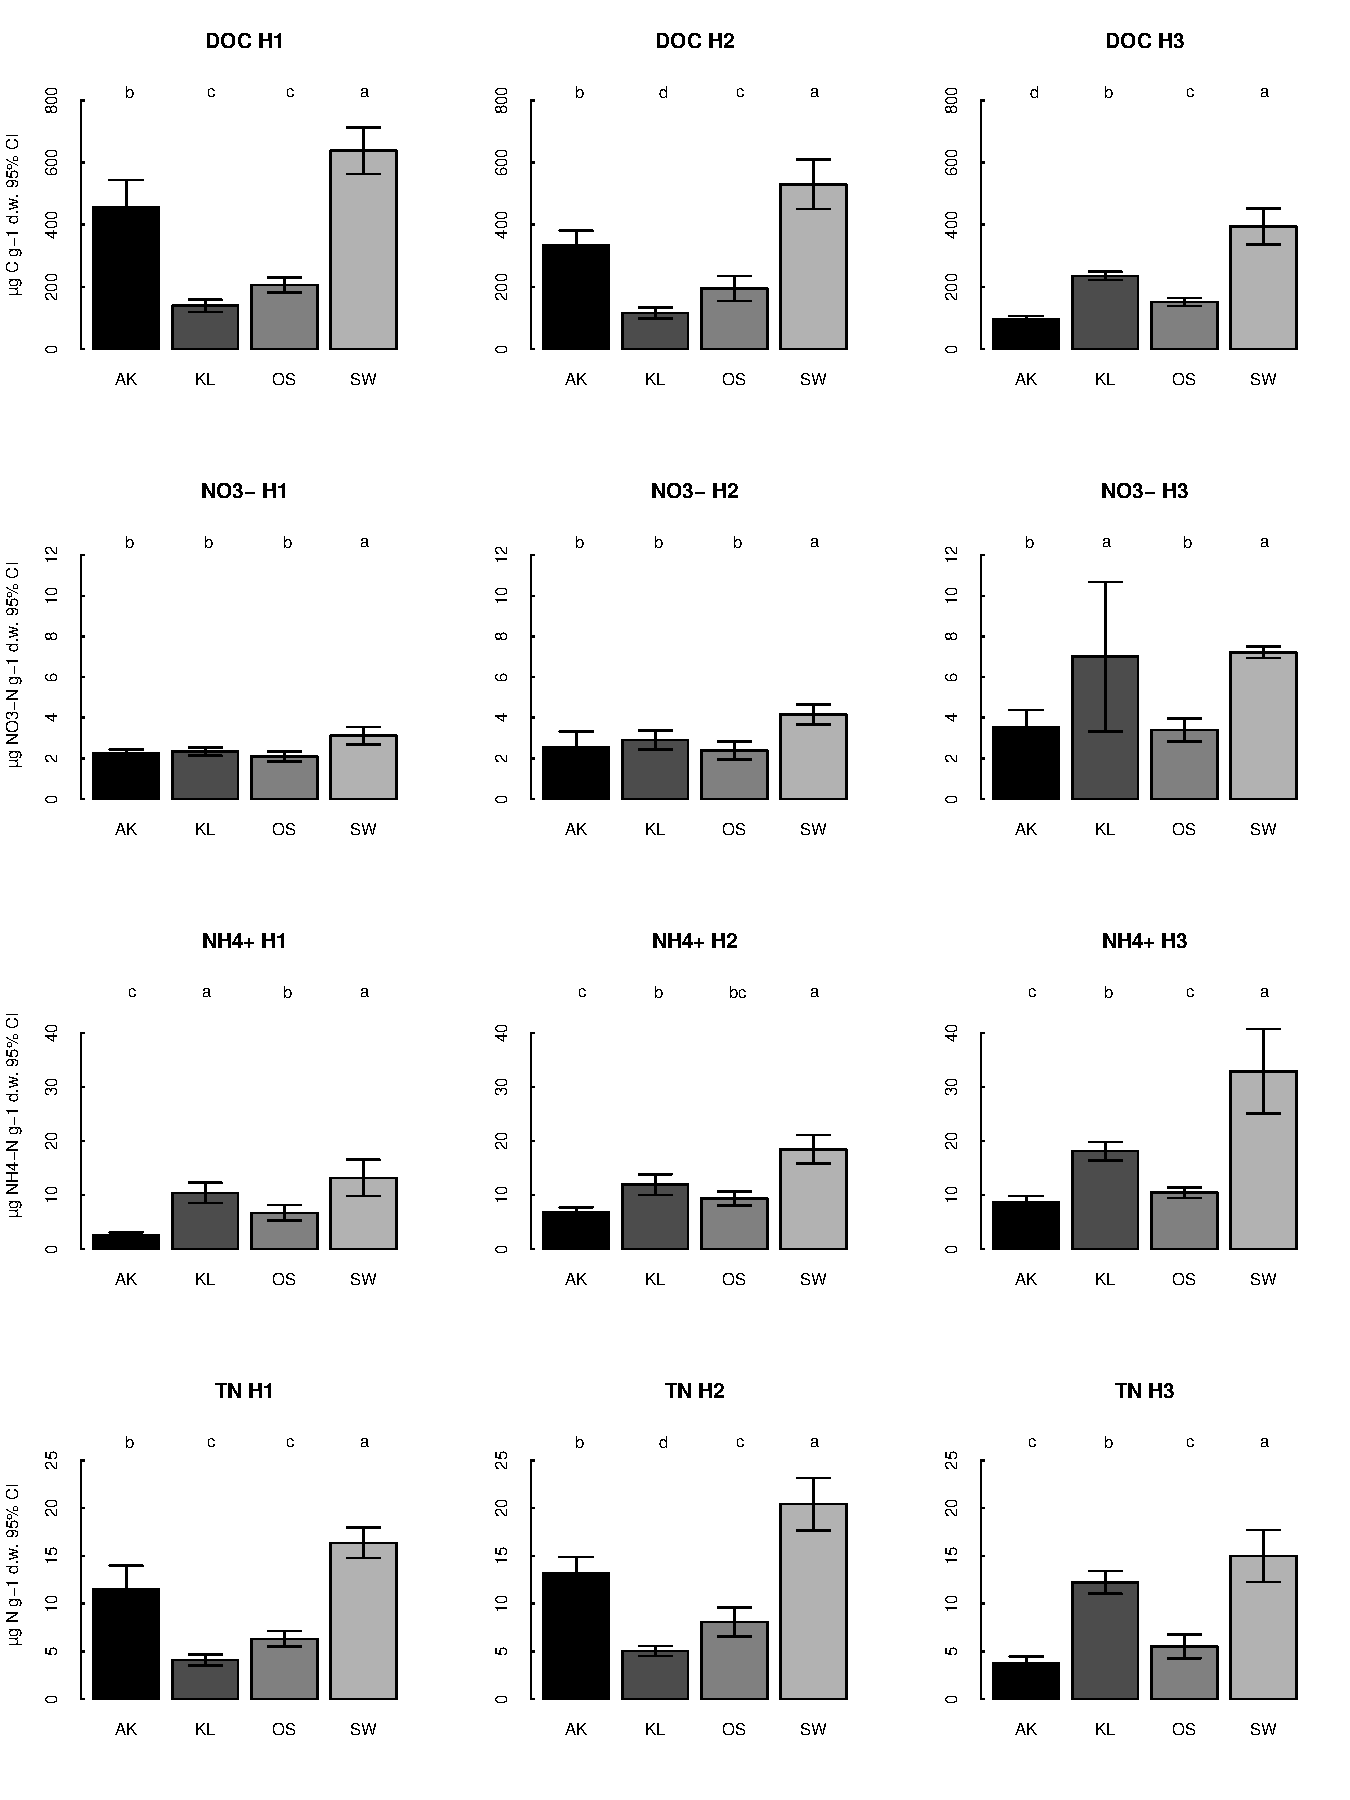
\includegraphics[width=15cm]{doc_barplots.pdf}
\end{center}
\caption{Litter Chemistry: Dissolved organic carbon, total dissolved nitrogen, NO3-, NH4+}
\end{figure*}

% \newpage
% \begin{figure*}[p]
% \vspace*{2mm}
% \begin{center}
% 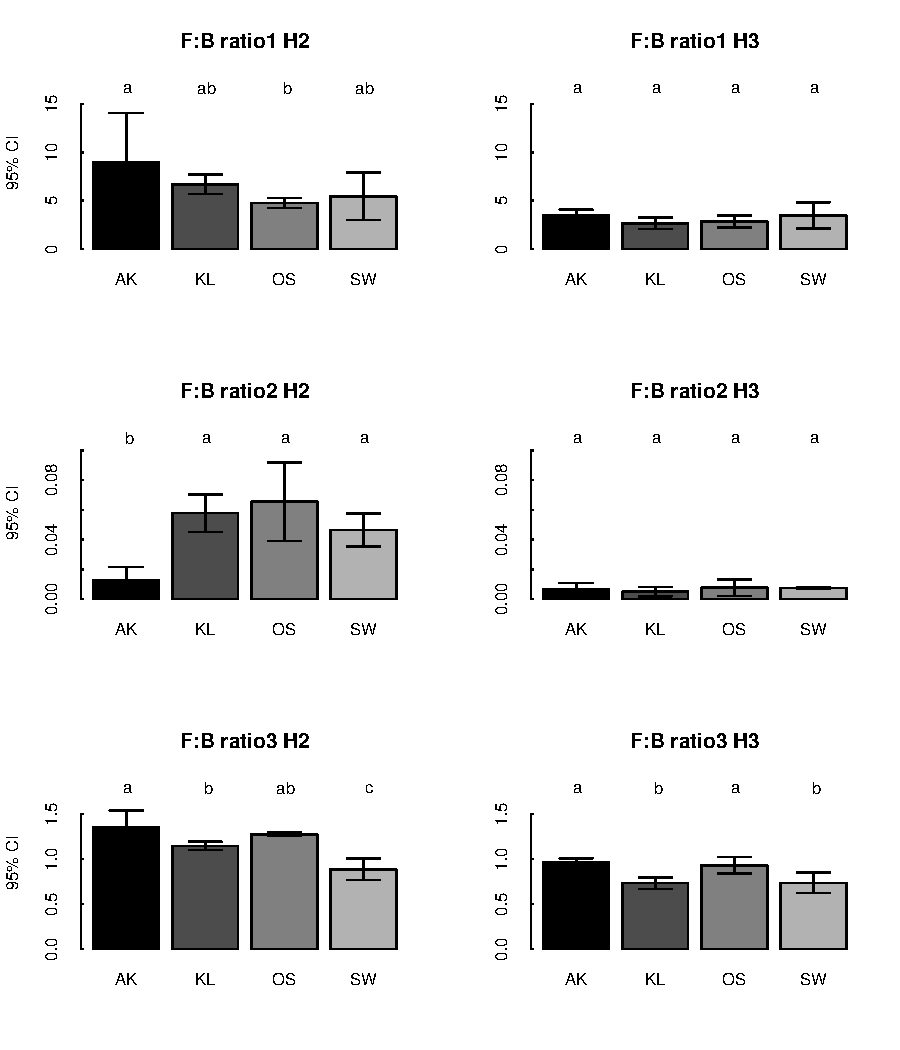
\includegraphics[width=12cm]{plfa.pdf}
% \end{center}
% \caption{Fungi : Bacteria ratios}
% \label{fig:plfa}
% \end{figure*}


%% Authors are advised to submit their bibtex database files. They are
%% requested to list a bibtex style file in the manuscript if they do
%% not want to use model2-names.bst.

%% References without bibTeX database:

% \begin{thebibliography}{00}

%% \bibitem must have one of the following forms:
%%   \bibitem[Jones et al.(1990)]{key}...
%%   \bibitem[Jones et al.(1990)Jones, Baker, and Williams]{key}...
%%   \bibitem[Jones et al., 1990]{key}...
%%   \bibitem[\protect\citeauthoryear{Jones, Baker, and Williams}{Jones
%%       et al.}{1990}]{key}...
%%   \bibitem[\protect\citeauthoryear{Jones et al.}{1990}]{key}...
%%   \bibitem[\protect\astroncite{Jones et al.}{1990}]{key}...
%%   \bibitem[\protect\citename{Jones et al., }1990]{key}...
%%   \harvarditem[Jones et al.]{Jones, Baker, and Williams}{1990}{key}...
%%

% \bibitem[ ()]{}

% \end{thebibliography}



\end{document}

%%
%% End of file `elsarticle-template-2-harv.tex'.
